\documentclass{article}
\usepackage{physics}
\usepackage{graphicx}
\usepackage{caption}
\usepackage{amsmath}
\usepackage{authblk}
\usepackage{amsfonts}
\usepackage{esint}
\usepackage{mathtools}
\usepackage{amsthm}
\theoremstyle{definition}
\newtheorem{defn}{Definition}[section]
\newtheorem{prop}{Proposition}[section]
\newtheorem{rmk}{Remark}[section]
\newtheorem{exmp}{Example}[section]
\usepackage{empheq}
\usepackage{hyperref}
\usepackage{tensor}
\usepackage{xcolor}
\hypersetup{
	colorlinks,
	linkcolor={black!50!black},
	citecolor={blue!50!black},
	urlcolor={blue!80!black}
}

\begin{document}
\begin{titlepage}\centering
 \clearpage
 \title{\textsc{\bf{GENERAL RELATIVITY\\ \& COSMOLOGY}}\\\smallskip A Quick Guide\\}
 \author{\bigskip Huan Bui}
 \affil{Colby College\\Physics \& Statistics\\Class of 2021\\}
 \date{\today}
 \maketitle
 \thispagestyle{empty}
\end{titlepage}

\subsection*{Preface}
\addcontentsline{toc}{subsection}{Preface}

Greetings,\\

\textit{General Relativity \& Cosmology - A Quick Guide to} is compiled from my PH335: General Relativity and Cosmology with professor Robert Bluhm at Colby College. The course is based on \textit{A Short Course in General Relativity}, 3$^{\text{th}}$ Edition, by James Foster and J. David Nightingale.\\

One of my favorite things to do is to transfer my handwritten lecture notes into nice \LaTeX documents. I started working on these documents last year with \textit{Special Relativity - A Quick Guide to}, which was based on (part of) my PH241: Modern Physics I with professor Charles Conover. I am still working on it, along with another one on Linear Algebra (based on MA253 with Otto Bretscher), and of course General Relativity - the one you are reading now. All of these .pdf files can be found on my \href{www.huanqbui.com}{website}, under the ``A Quick Guide to...'' tab. For the ``raw'' content, i.e., my handwritten lecture notes, feel free to visit the ``Lecture Notes'' tab.\\

Today is Dec 22, 2018. In the spring I will be doing an independent study on Classical Fields Theory with prof. Bluhm. I will also be taking Matrix Analysis with prof. Leo Livshits. I'm excited to be taking these advanced physics and mathematics courses, and I look forward to sharing my journey with you through my lecture notes.  \\

Enjoy!

\newpage
\tableofcontents
\newpage

\section{Overview and Review}

General relativity is a theory of gravity, replacing Newton's gravity law for heavy masses to give more precise predictions. However, we should keep in mind that general relativity is not yet compatible with quantum mechanics. There are numerous open problems in physics related to reconciling gravity and quantum mechanics. 

\subsection{Review of Special Relativity}

Special relativity studies the kinematics and dynamics in relatively moving inertial reference frames. Most of special relativity and its consequences are encoded in the Lorentz transformations. A classic example of a Lorentz transformation that is often focused on in introductory special relativity is called the ``Lorentz boost'' in the $x$-direction. Note that there is nothing special about $x$ or $y$ or $z$. The $x$-Lorentz boost is essentially a coordinate transformation, i.e. given coordinates an event $A$ in frame $(S)$, we can calculate the coordinates of $A$ in frame $(S')$.
\begin{align*}
\begin{pmatrix}
ct'\\x'\\y'\\z'
\end{pmatrix}
=
\begin{pmatrix}
\gamma & -\gamma\beta & 0 & 0\\
-\gamma\beta & \gamma & 0 & 0\\
0 & 0 & 1 & 0\\
0 & 0 & 0 & 1
\end{pmatrix}
\begin{pmatrix}
ct\\x\\y\\z
\end{pmatrix}
=
\begin{pmatrix}
ct\\x\\y\\z
\end{pmatrix},
\end{align*}
where $\beta = v/c$ and the Lorentz factor 
\begin{align*}
\gamma = \frac{1}{\sqrt{1-\frac{v^2}{c^2}}}.
\end{align*}
Since we are studying relativity, it is important to look at ``invariants'' - quantities that do not change under transformations. In special relativity, one such invariant is the spacetime invariant:
\begin{align*}
(\Delta S)^2 &= (c\Delta \tau)^2\\
&= (c\Delta t)^2 - (\Delta x)^2 - (\Delta y)^2 - (\Delta z)^2\\
&= (c\Delta t')^2 - (\Delta x')^2 - (\Delta y')^2 - (\Delta z')^2\\
&= (\Delta S')^2 = (c\Delta \tau')^2.
\end{align*}
This can be readily shown. In fact, we have verified this in \textit{Special Relativity: A Quick Guide}. This quantity, roughly speaking, is a measure of \textbf{proper} distances and times. If we go to a rest frame of event $A$, such that $\Delta x' = \Delta y' = \Delta z' = 0$, then we get $\Delta t' = \Delta \tau$, where $\tau$ denotes the \textbf{proper time}, which is the time measured in the rest frame. This gives $(\Delta S)^2 = (c\Delta \tau)^2$.\\

In relativity in general and in Minkowski spacetime in particular, we are interested in two types of objects: \textbf{scalars} and \textbf{vectors}. Scalars are invariant under general coordinate transformations. An example of a scalar is the spacetime invariant. Another scalar, which we probably will not see again in this text, is the metric signature (sgn($[\eta_{\mu\nu}] = -2$)). Vectors, on the other hand, are a different type of objects, which transform in the same way under coordinate transformations, but are not invariant under general coordinate transformations in general, i.e., their components are not necessarily the same in different coordinate systems. In 4-dimensional spacetime, we work with 4-vectors, which simply means 4-component vectors.\\

In special relativity, we often talk about position vectors $\mathbf{x} = (ct,x,y,z)^\top = (ct,\vec{x})^\top$ and energy-momentum vectors $\mathbf{p} = (E/c,p_x,p_y,p_z)^\top = (E/c, \vec{p})^\top$. These vectors transform under the Lorentz transformation. 
\begin{exmp}
The $x$-Lorentz boost applied to $\mathbf{p}$ gives
\begin{align*}
\begin{pmatrix}
E'/c\\p_x'\\p_y'\\p_z'
\end{pmatrix}
=
\begin{pmatrix}
\gamma & -\gamma\beta & 0 & 0\\
-\gamma\beta & \gamma & 0 & 0\\
0 & 0 & 1 & 0\\
0 & 0 & 0 & 1
\end{pmatrix}
\begin{pmatrix}
E/c\\p_x\\p_y\\p_z
\end{pmatrix}.
\end{align*}
Notice that $E/c$ transforms like $ct$ (time) and $\vec{p}$ transforms like $\vec{x}$ (space). We also have the following invariant
\begin{align*}
\frac{E^2}{c^2} - p^2_x - p^2_y - p^2_z = \frac{E^2}{c^2} - \vec{p}\cdot\vec{p}.
\end{align*}
But recall that $(mc)^2 = E^2/c^2 - \vec{p}\cdot\vec{p}$, so
\begin{align*}
\frac{E^2}{c^2} - p^2_x - p^2_y - p^2_z = (mc)^2.
\end{align*} 
If we go to a rest frame, such that $\vec{p} = \vec{0}$, then we obtain the famous rest mass-energy equivalence: $E = mc^2$.
\end{exmp}
Some quantities associated with a vector can be invariant (scalar), such as their norm. In fact, the spacetime invariant in Minkowski space is nothing but a dot product of a vector with itself:
\begin{align*}
\mathbf{a}\cdot\mathbf{a} = a^0a^0 - a^1a^1 - a^2a^2 - a^3a^3,
\end{align*}
where $0,1,2,3$ are indices, and $\mathbf{a}$ implies a 4-vectors, which should be distinguished from the 3-vector $\vec{a} = (a^1,a^2,a^3)^\top$. Notice that the dot product in Minkowski spacetime is defined differently from that in flat 3-dimensional Cartesian coordinate system. In the following chapters, we will explore how dot products are defined in general. Hint: the metric tensor plays an important role.\\ 


\subsection{The Equivalence Principle}
In 1907, Albert Einstein had the ``happiest thought of his life'' when he realized that in a freely falling frame (non rotating and/or accelerating), the effects of gravity go away, i.e., there is an equivalence between gravity and acceleration such that they can ``undo'' each other. For example, the following two situations are equivalent in terms of the acceleration experienced by the observer: (i) a person standing on Earth, and (ii) a person inside an elevator accelerating upwards at rate $g$ in free space (no gravitational field). Likewise, the following two situations are also equivalent: (iii) a person floating in free space, and (iv) a person inside an airplane free falling towards Earth (this is commercially known as ``zero-G flight''). we arrive at the statement of the Equivalence Principle: \\

\noindent \boxed{``\textit{A small, non-rotating, freely falling frame in a $\vec{g}$ field is an inertial frame.}''}\\

The above statement is a direct result of Galileo's discovery that all objects have the same acceleration due to gravity. This result may seem a little bit \textit{circular}, because it is actually a coincidence that the two roles of \textbf{mass}: (i) to cause gravitational force like charge in an electric field:
\begin{align*}
\vec{F} = \frac{GMm_G}{r^3}\vec{r} = m_G\vec{g}
\end{align*}
and (ii) to measure inertia:
\begin{align*}
\vec{F} = m_I\vec{a}
\end{align*}
are the same, i.e., $m_I = m_G$. It could have been that ``gravitational mass'' $m_G$ and ``inertial mass'' $m_I$ are not the same, in which case $\vec{a} \neq \vec{g}$, and the equivalence principle does not hold. However, the famous E\"{o}tv\"{o}s experiment, which measured the correlation between inertial mass and gravitational mass, has shown that
\begin{align*}
\frac{\vert m_G - m_I\vert}{m_I} \leq 10^{-10}.
\end{align*}

While the observations we have made so far can seem self-apparent, the consequence of the equivalence principle is the bending of light around massive objects. Consider a light ray going horizontally (left to right) pass an upward-accelerating elevator with an observer inside. For the observer, since he is accelerating upwards, he sees the light beam as bent, entering at the top-left of the elevator and exiting at the bottom-right. Now, according to the equivalence principle, because the upward-accelerating scenario is equivalent to the existence of a massive object (such that the observer experiences the same acceleration). This means that the observer, now no longer in the elevator, ``sees'' the light as bent around this massive object. Fig. 1. illustrates this postulate.\\
\begin{figure}[h!]
	\centering
	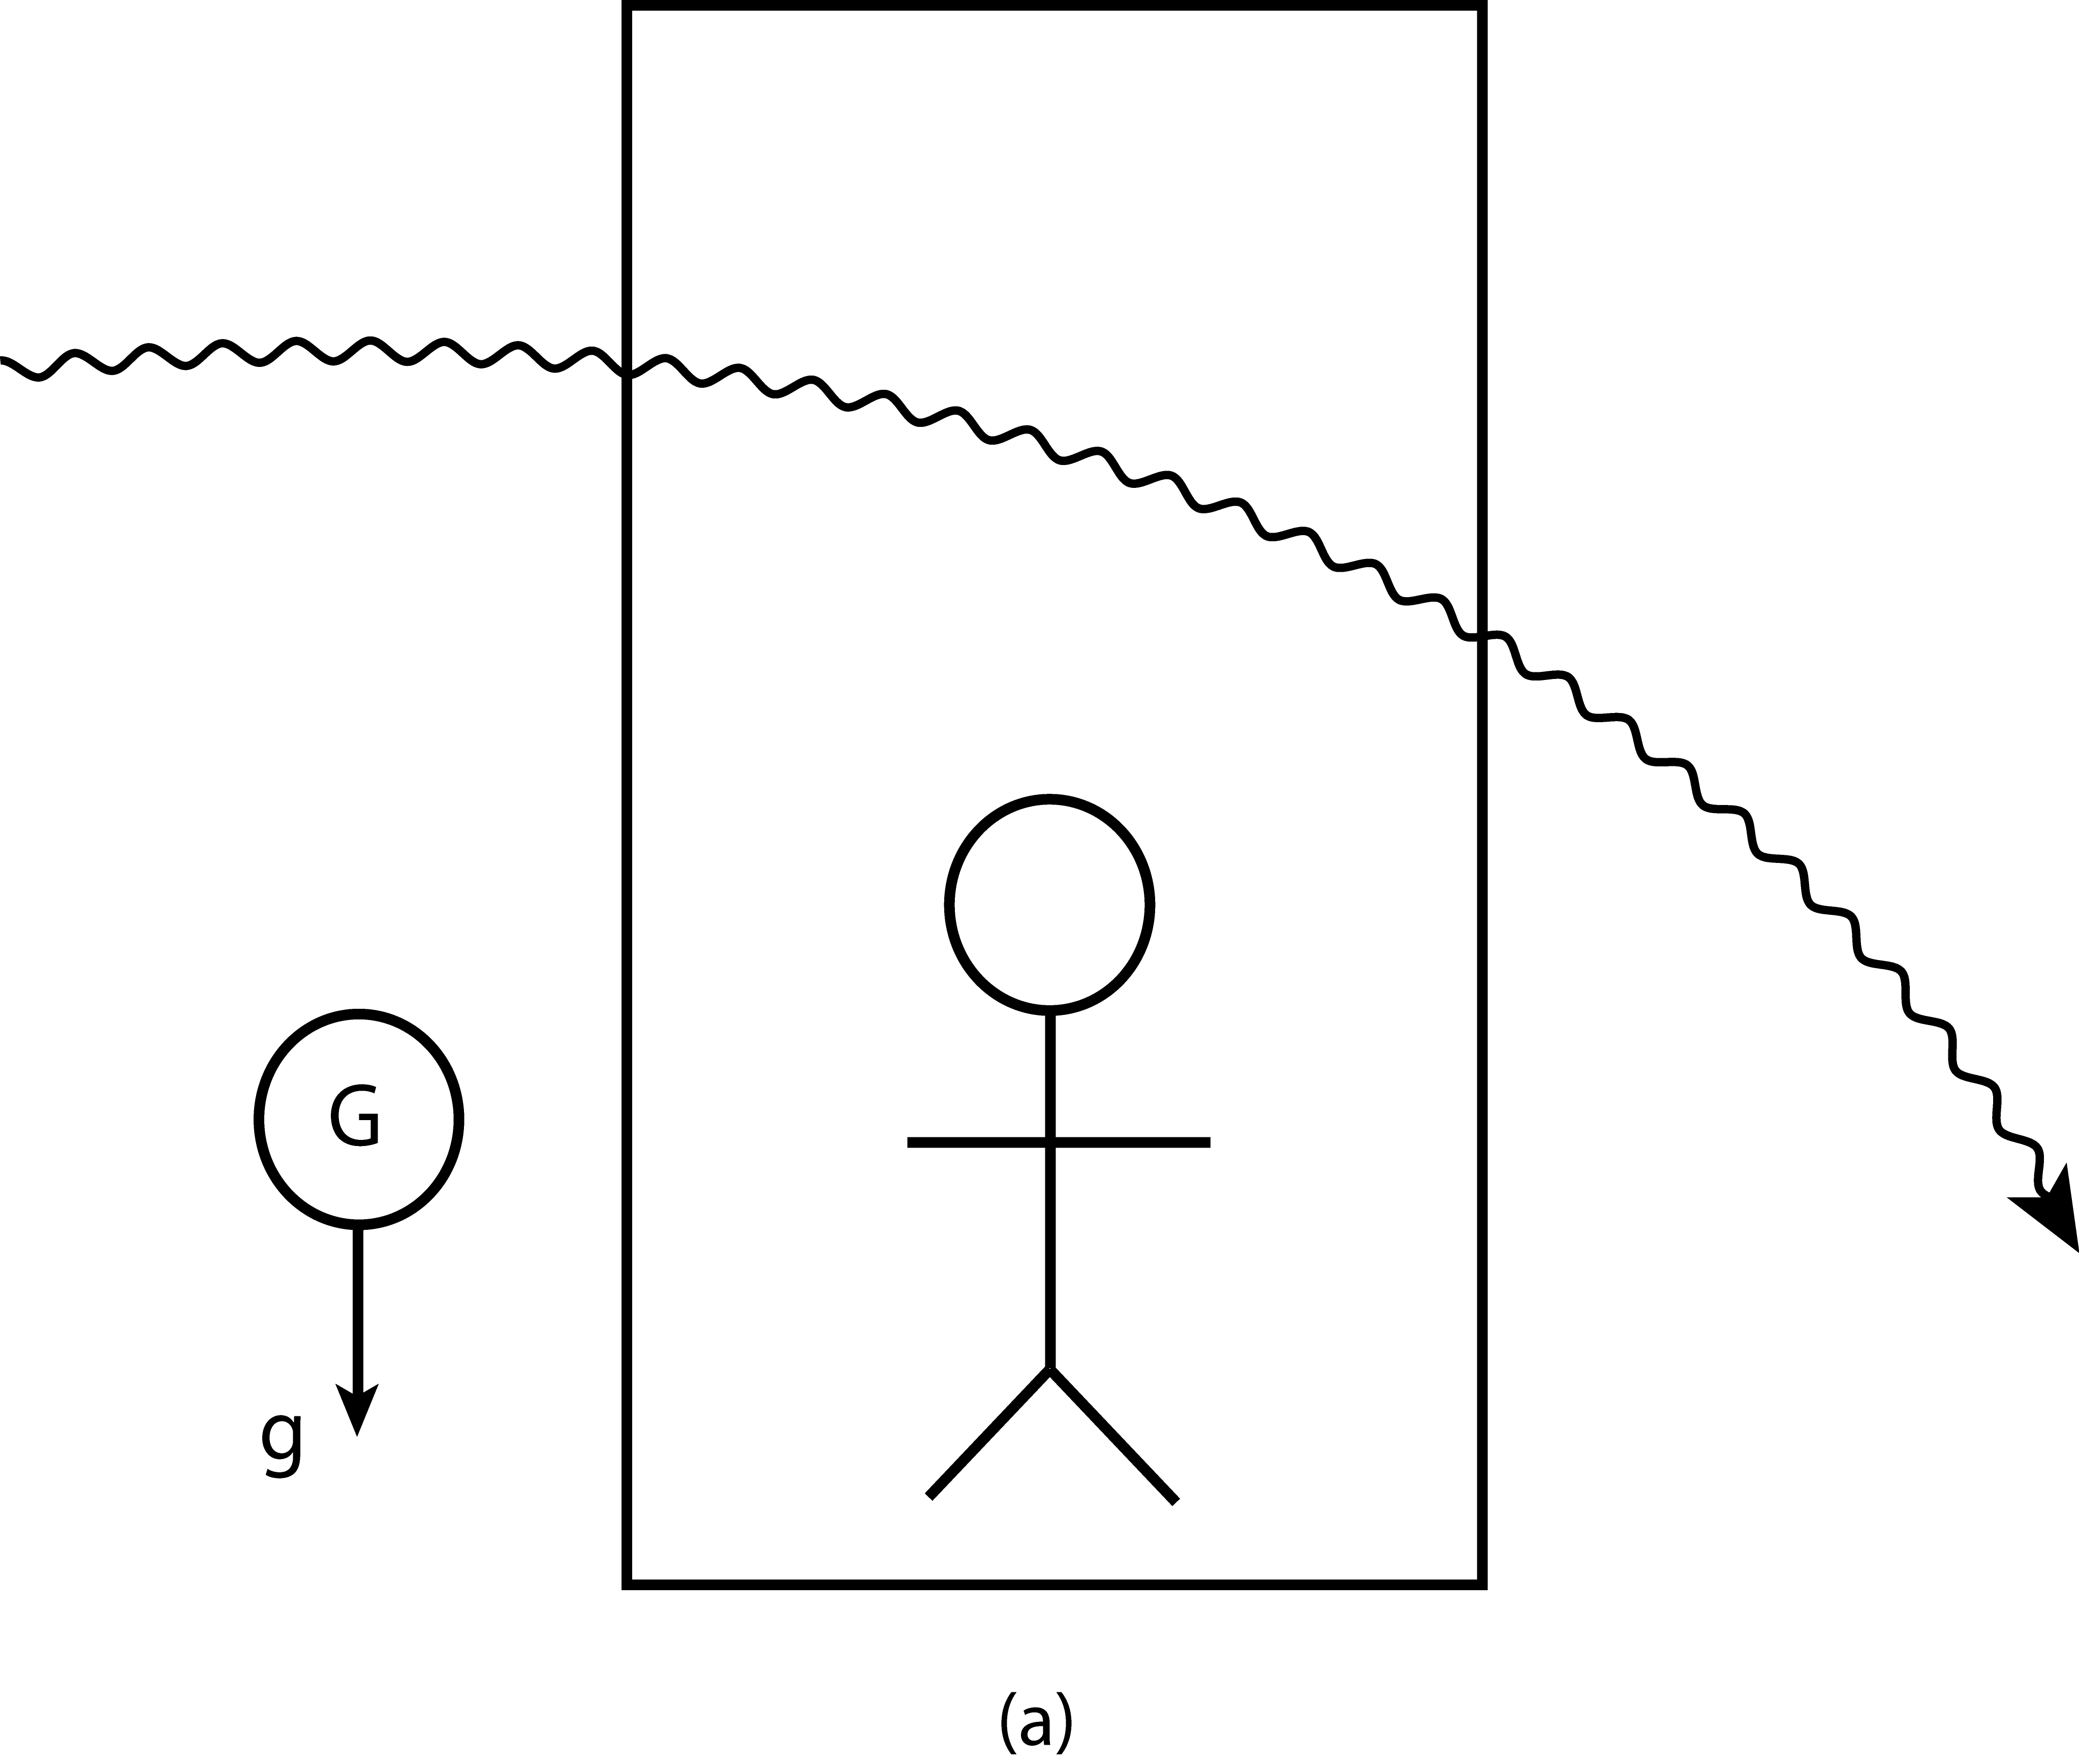
\includegraphics[scale=0.15]{gr-fig-1a.png}
	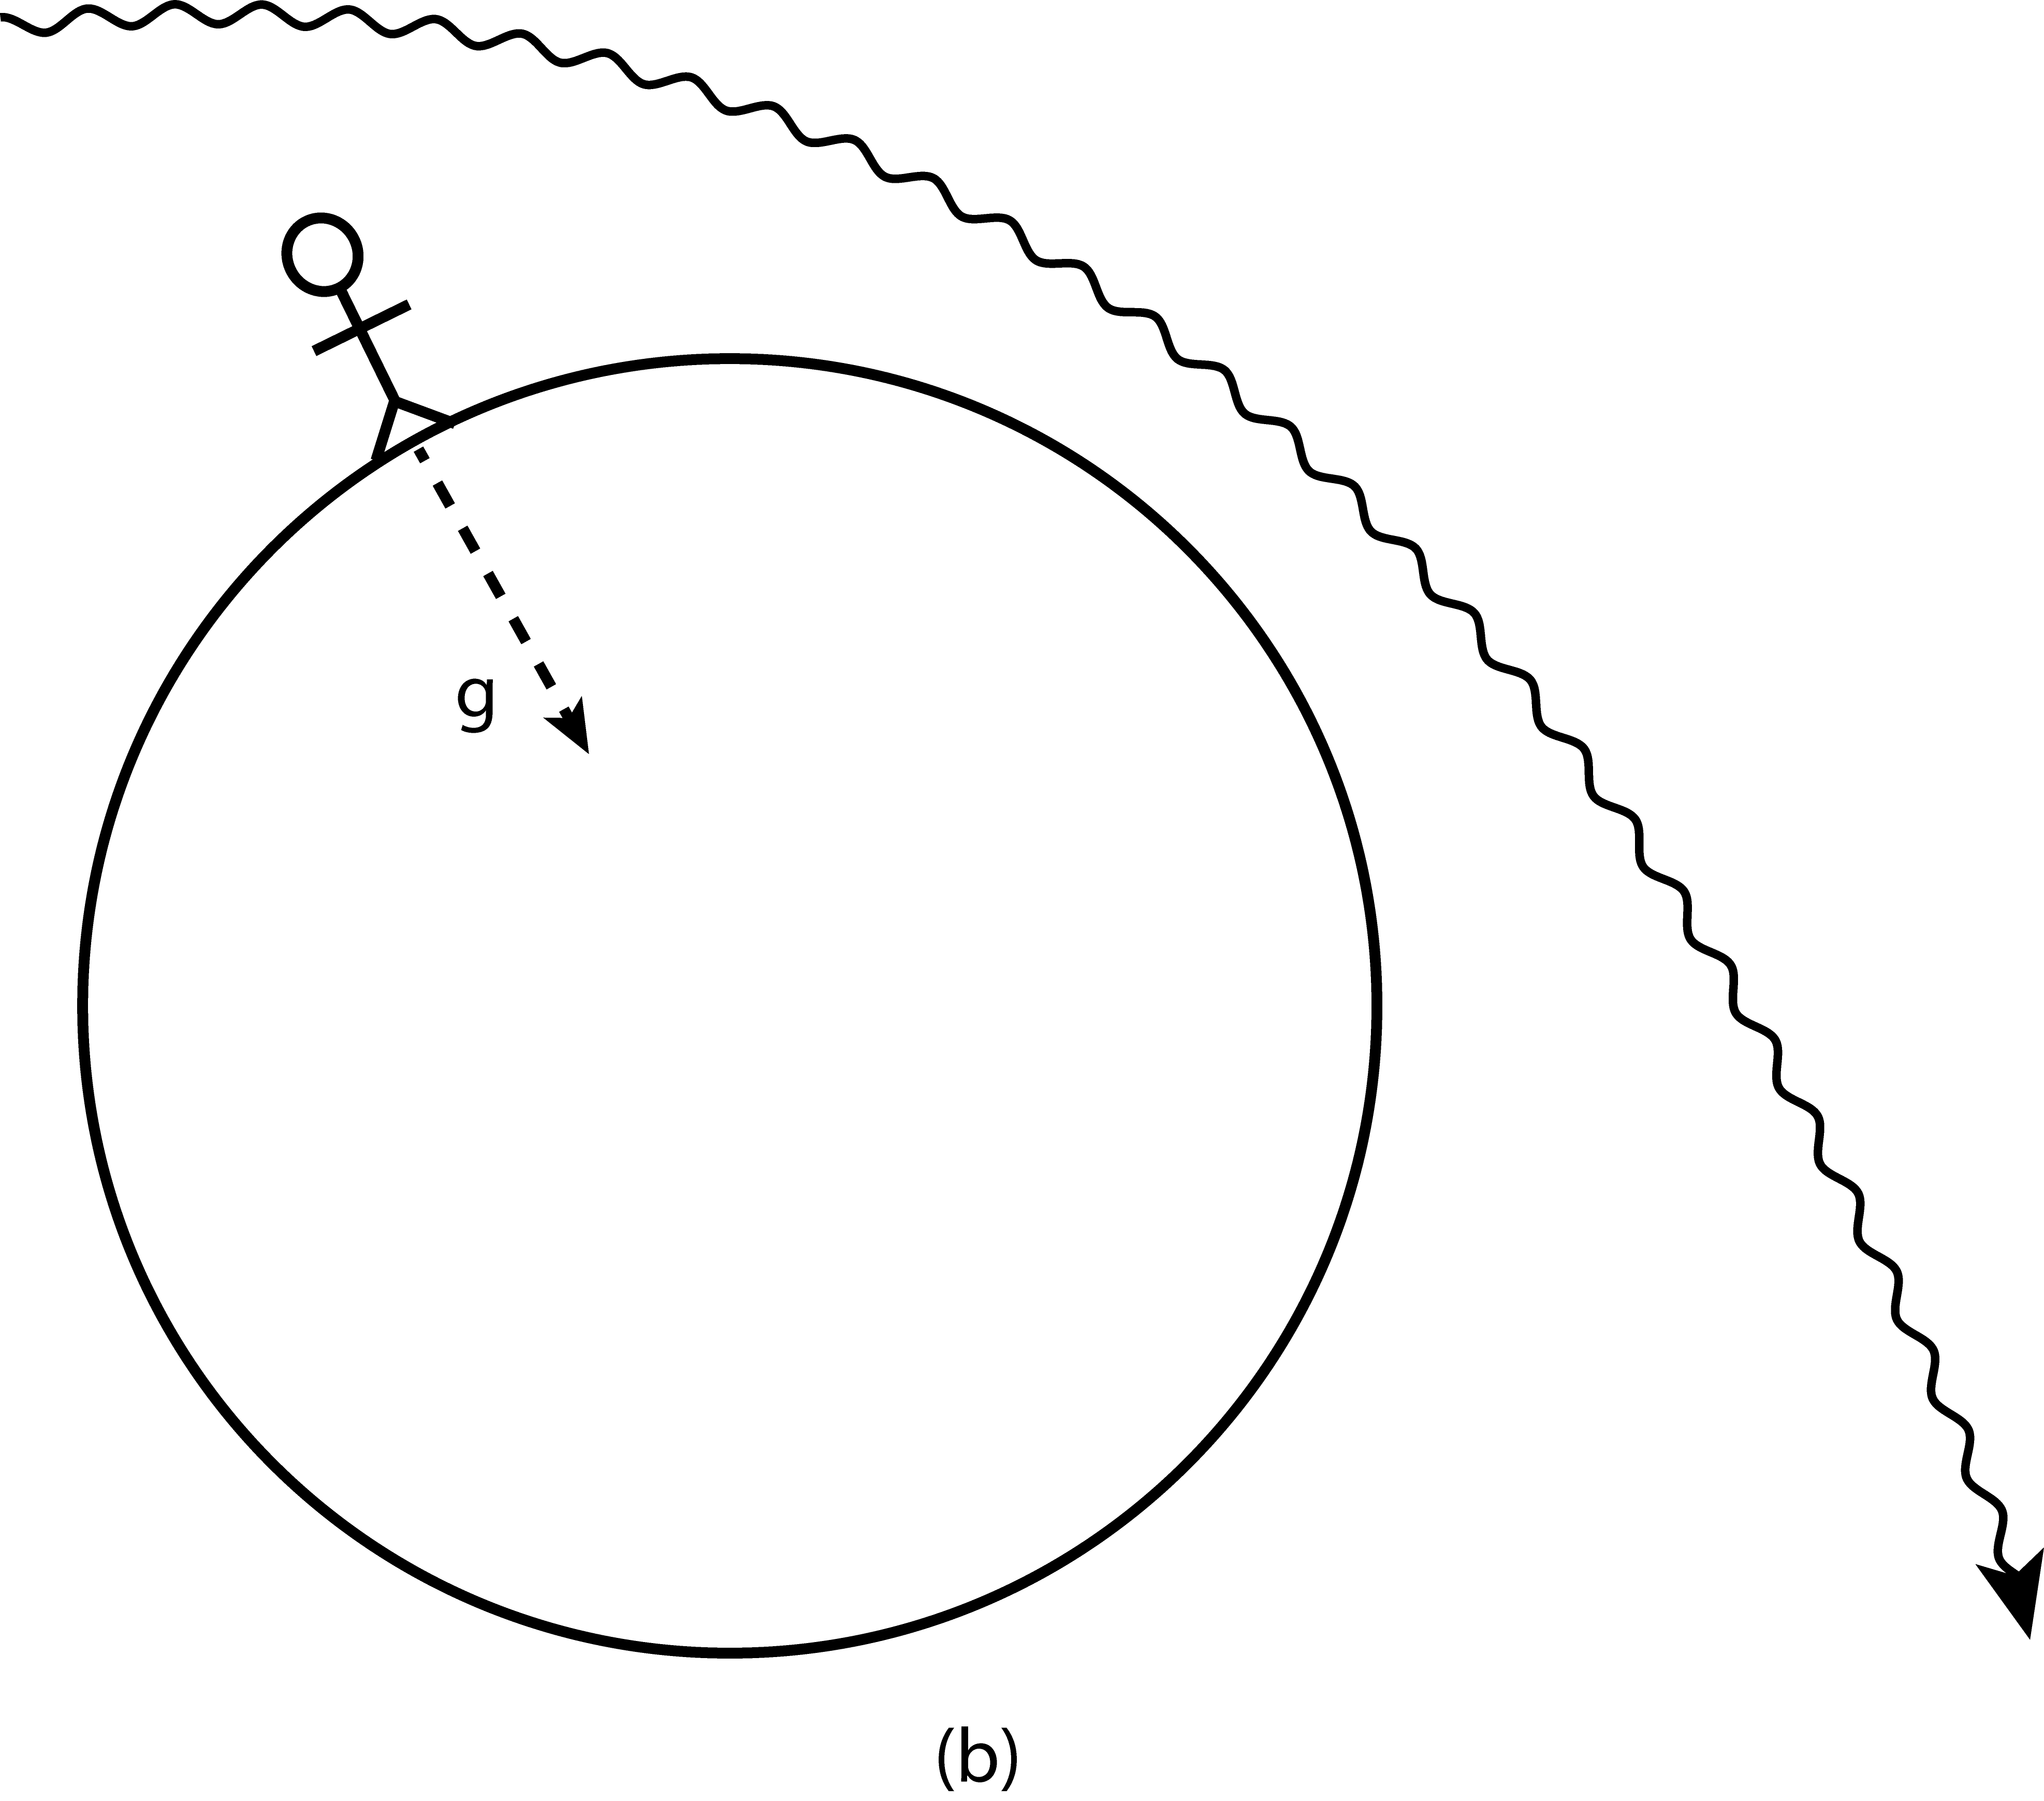
\includegraphics[scale=0.15]{gr-fig-1b.png}
	\caption{(a) A person in an upward-accelerating elevator (hence ``Ground'' is downward-accelerating at rate $g$) sees light as bent. (b) A person on a massive planet also sees light as bent.}
\end{figure}

General relativity predicts that light going pass Earth's surface will ``fall'' by approximately $1 \text{\AA}$, which is not observable. However, for a much more massive object like the Sun, general relativity predicts a bending of $1.75''$ (arc sec). This prediction was verified by the glorious experiment of Arthur Eddington.\\

Note that we could argue for the bending of light, using Newtonian physics. However, in order to get the correct predictions for the bending of light, we need general relativity. We will explore the reason behind this discrepancy in the following chapter. But roughly speaking, spacetime is assumed to be flat in Newtonian physics, while spacetime is curved by massive objects, according to general relativity. One might ask: ``How do we view falling objects on Earth as due to the curvature of spacetime?'' The answer requires bringing back Minkowski spacetime diagrams.
\begin{figure}[h!]
	\centering
	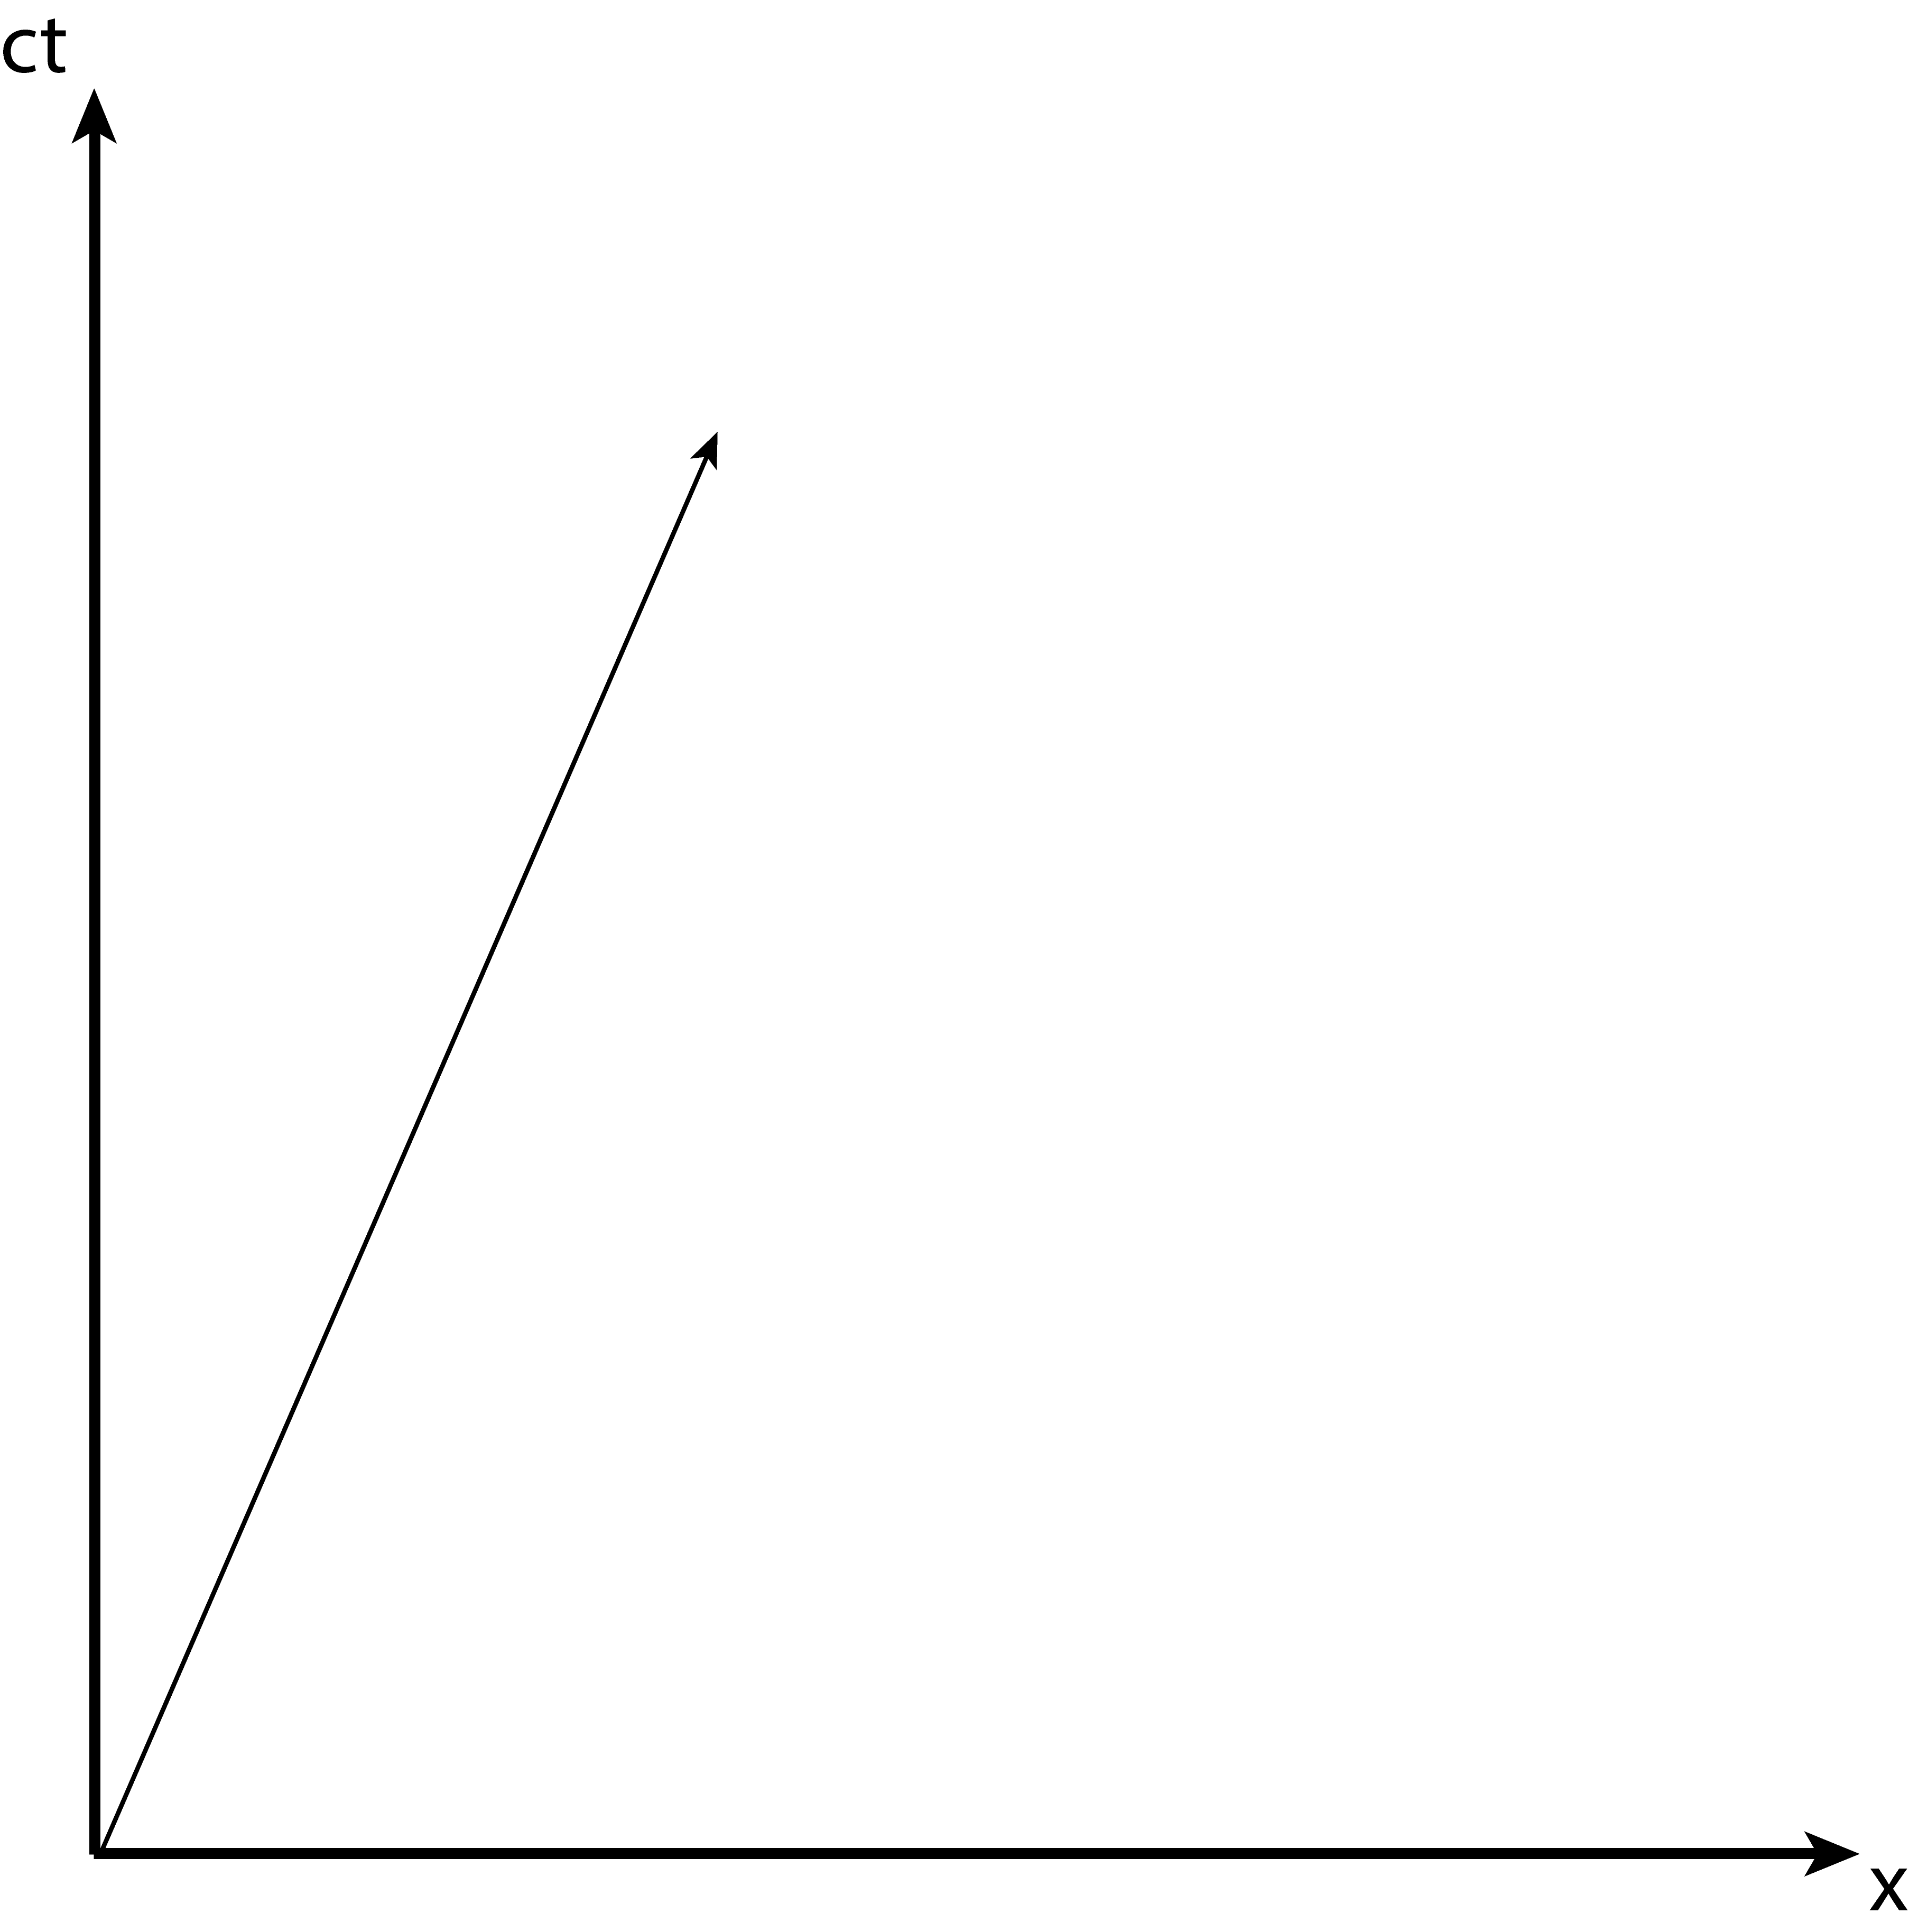
\includegraphics[scale=0.15]{gr-fig-2a.png} 
	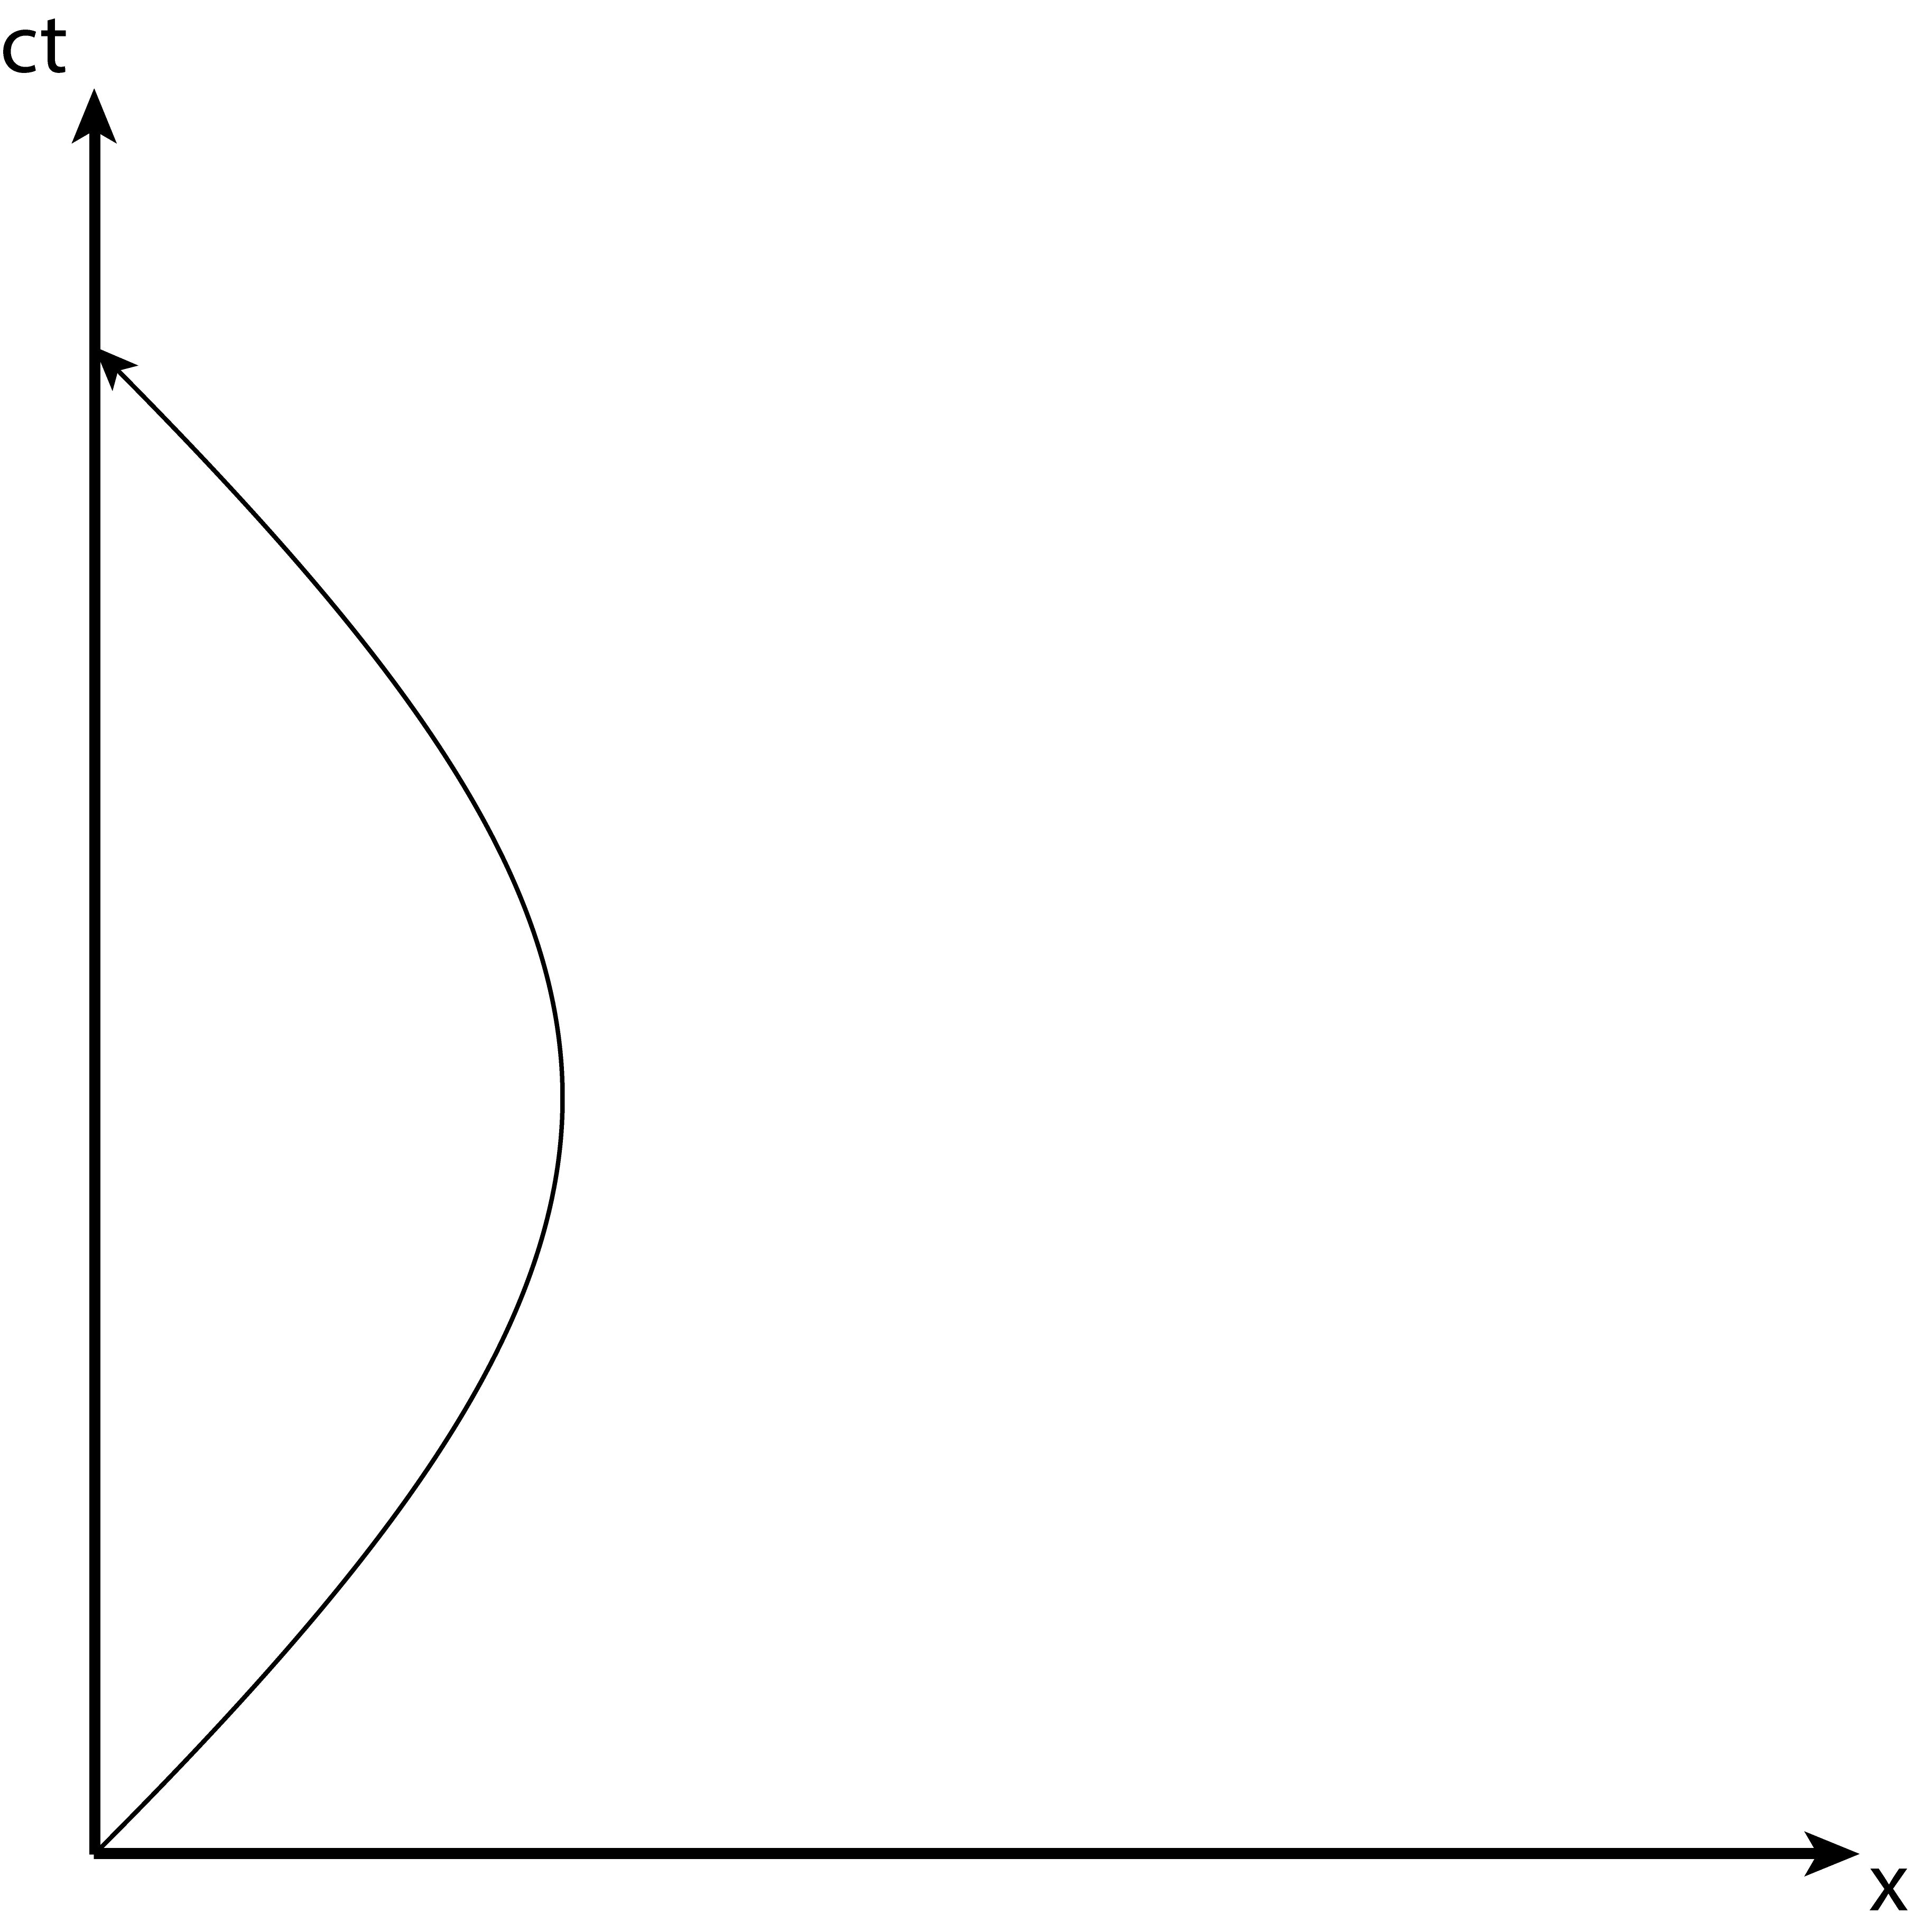
\includegraphics[scale=0.15]{gr-fig-2b.png}
	\caption{World-lines of an object traveling at constant velocity $v$ and of an object that is falling. Note that the ``curvature'' due to $g$ here is extremely exaggerated.}
\end{figure}

\subsection{Versions of the Equivalence Principle}
There are two versions of the equivalence principle, referred to as the \textit{strong equivalence principle}, SEP, and the \textit{weak equivalence principle}, WEP. 
\subsubsection{The Strong Equivalence Principle}
The strong equivalence principle states that \textbf{all} of physics reduces to special relativity in a freely falling frame.
\subsubsection{The Weak Equivalence Principle}
The weak equivalence principle states that all point particles fall at the same rate in a gravitational field ($m_G = m_I$). We notice that WEP only applies to gravity, which makes it sufficient to develop general relativity, but not quantum mechanics. For this remaining of this note, we will rely on the WEP. 

\newpage

\section{Review of Vector Calculus}
\subsection{Operations \& Theorems}
Recall that a path in 3-dimensional space can by parameterized a single variable, which we will call $t$, as
\begin{align*}
\vec{r}(t) = x(t)\hat{i} + y(t)\hat{j} + z(t)\hat{k},
\end{align*}
where the tangent to this path is given by
\begin{align*}
\dot{\vec{r}}(t) = \frac{d \vec{r}}{dt}.
\end{align*}
The length of the underlying curve of this path is the integral over the line element $ds = \vert\vert \vec{r} \vert\vert = \vert\vert \dot{\vec{r}} \vert\vert\,dt$:
\begin{align*}
L = \int_{a}^{b} dS = \int_{a}^{b} \vert\vert \dot{\vec{r}} \vert\vert\,dt.
\end{align*} 
\begin{exmp}
Consider a path in $\mathbb{R}^2$ defined as $\vec{r}(t) = (t, \sin t)$, with $t \in [-2\pi, 2\pi]$. We instantly recognize that the underlying curve of this path is nothing but a sine curve in the $xy$-plane. The length of this curve is
\begin{align*}
L = \int_{-2\pi}^{2\pi}\vert\vert  (1,\cos t)\vert\vert\,dt  = \int_{-2\pi}^{2\pi} \sqrt{1+\cos^2 t}\,dt \approx 15.28.
\end{align*}
\end{exmp}
Next, we consider a vector-valued function $\vec{F} : \mathbb{R}^3 \rightarrow \mathbb{R}^3$ defined as $\vec{F}(\vec{r}) = (F_x(x,y,z), F_y(x,y,z),F_z(x,y,z))$. Recall the two ``del operators'' from vector calculus: the \textbf{curl} and the \textbf{div}, whose definitions are
\begin{align*}
\text{curl}(\vec{F}) = \vec{\nabla} \times \vec{F} = \det
\begin{pmatrix}
\hat{i} & \hat{j} & \hat{k} \\
\frac{\partial}{\partial x} & \frac{\partial }{\partial y} & \frac{\partial}{\partial z}\\
F_x & F_y & F_z
\end{pmatrix}
\end{align*}
and 
\begin{align*}
\text{div}(\vec{F}) = \vec{\nabla} \cdot \vec{F} = 
\frac{\partial F_x}{\partial x} + \frac{\partial F_y }{\partial y} + \frac{\partial F_z}{\partial z}.
\end{align*}
where the ``del'' symbol represents the operator
\begin{align*}
\vec{\nabla} = \left( \frac{\partial }{\partial x} , \frac{\partial }{\partial y} , \frac{\partial }{\partial z} \right). 
\end{align*}
We have also seen the \textbf{gradient} of a scalar field (or potential) $f : \mathbb{R}^3 \rightarrow \mathbb{R}$. The gradient is defined as
\begin{align*}
\vec{\nabla}f = \left( \frac{\partial f}{\partial x} , \frac{\partial f }{\partial y} , \frac{\partial f}{\partial z}\right) .
\end{align*}
There are two kinds of potential functions in vector calculus: scalar potential and vector potential. While we are more familiar with the scalar potential (e.g. the gravitational potential or the electric potential in electromagnetism), there isn't as strong a connection between vector potentials and any physical meaning. However, we should still look at some examples. 
\begin{exmp}
In electromagnetism, an electric field $\vec{E}$ is defined as the negative gradient of the electric potential $\phi$, measured in Volts:
\begin{align*}
\vec{E} = -\vec{\nabla}\phi.
\end{align*}
On the other hand, an magnetic field $\vec{B}$ is defined as the curl of the magnetic potential $\vec{A}$.
\begin{align*}
\vec{B} = \vec{\nabla}\times\vec{A}.
\end{align*}
In this case, $A$ is a vector potential. Note that we don't often talk about a vector potential of an electric field. This is simply because for a point charge, which produces an inverse-square field, the vector potential simply does not exist. The proof is straightforward. For curious readers, this proof can be an interesting exercise (the solution should be a one-liner). Or else, please refer to my vector calculus notes on my website. Hint: we need one of the two following fundamental theorems of vector calculus: Stokes' and Gauss' (or Ostrogradsky's).
\end{exmp}
\textbf{Stokes' theorem} states that, the circulation around a closed curved in $\mathbb{R}^3$ by a vector field $\vec{F}$ is the flux of $\vec{\nabla}\times\vec{F}$ through the surface $S$ whose boundary $C = \partial S$ is the curve $C$.
\begin{align*}\boxed{
\oint_{C = \partial S} \vec{F}\cdot\,d\vec{s} = \iint_{S} \vec{\nabla}\times \vec{F} \cdot\,d\vec{S}.}
\end{align*}

\textbf{Gauss' theorem} states that, if $S$ is closed surface, oriented outward, and if $\vec{F}$ is defined throughout the solid region $W$ enclosed by $S$, then the flux of $\vec{F}$ through $S$ is the total divergence of $S$ through the region $W$.
\begin{align*}
\boxed{
\oiint_{S=\partial W}\vec{F}\cdot\,d\vec{S} = \iiint \vec{\nabla}\cdot\vec{F}\,dV.}
\end{align*}
\textbf{Line integrals} are one of a few important operations in vector calculus. In the context of undergraduate or high school physics, we often use the line integral to calculate the work done by a force $\vec{F}$ over some path $\vec{r}$. The integral in general is simply an accumulation of the component of the vector field along the path. 
\begin{align*}
\int_{a}^{b}\vec{F}\cdot\,d\vec{r}.
\end{align*} 
If $\vec{F}$ is a conservative field, then the line integral along $\vec{F}$ between two point $A$ and $B$ only depends on where $A$ and $B$ are, i.e., the line integral is path-independent. A good illustration of this fact is the way we compute the change in electric potential:
\begin{align*}
W = -\int \vec{E}\cdot\,d\vec{r} = \Delta \phi
\end{align*}

To actually compute a line integral, we often look for symmetry first (or whether $\vec{F}$ is conservative), then parameterize $\vec{r} = \vec{r}(s)$ if we must. Then, the line integral becomes
\begin{align*}
\int_{a}^{b}\vec{F}\cdot\,d\vec{r} = \int_{a}^{b}\vec{F}(\vec{r}(s))\cdot \frac{d\vec{r}}{ds}\,ds
\end{align*}
\textbf{Surface integrals} give the flux of a vector field through a surface:
\begin{align*}
\int \vec{F}\cdot\,d\vec{S} = \int\vec{F}\cdot\vec{n}\,dS = \pm\int\vec{F}\cdot\vec{N}\,d\phi,d\theta,
\end{align*}
where $\vec{F}$ is the vector field, and $\vec{n}$ is the unit normal vector to the surface. The last expression denotes the surface integral in terms of a parameterization $\vec{S}(\phi, \theta) = (x(\phi, \theta),y(\phi, \theta),z(\phi, \theta))$. $\vec{N}$ is the standard normal to the surface, which is not necessarily a unit vector (with norm of 1) and not necessarily in the same direction as $\vec{n}$, which is intrinsic to the surface.
\begin{exmp}
Consider the electric flux through a sphere:
\begin{align*}
\Phi_E = \oiint\vec{E}\cdot\,d\vec{a} = \frac{q}{\epsilon_0}.
\end{align*}
The last expression comes from Gauss' (or Ostrogradsky's) theorem, equivalently the divergence theorem, where $q$ is the charge enclosed.
\end{exmp}
We should introduce the Maxwell's equations as they ``bring together'' the concepts we have touched on so far. To see how, we consider the Maxwell's equations in integral form:
\begin{align*}
\text{Gauss' law:  } \Aboxed{&\oiint\vec{E}\cdot\,d\vec{a} = \frac{q}{\epsilon_0}}\\
\text{No magnetic monopole:  } \Aboxed{&\oint\vec{B}\cdot\,d\vec{a} = 0}\\
\text{Faraday's law:  } 
\Aboxed{&\oint \vec{E}\cdot\,d\vec{s} = -\frac{d}{dt}\Phi_B = \frac{\partial}{\partial t}\int_A\vec{B}\cdot\,d\vec{a}}\\  
\text{Ampere-Maxwell's law:  } 
\Aboxed{&\oiint \vec{B}\cdot\,d\vec{s} = \mu_0I + \mu_0\epsilon_0\frac{\partial}{\partial t}\int_A\vec{E}\cdot\,d\vec{a}}
\end{align*}
Using the theorems and facts we have discussed, we can convert the above equations into differential form. First, we can use Gauss' theorem on Gauss' law, with
\begin{align*}
q = \int_V \rho\,d^3r
\end{align*}
where $\rho$ is the charge volume density. So, Gauss' law becomes
\begin{align*}
\oint \vec{E}\cdot\,d\vec{a} = \int_V \vec{\nabla}\cdot\vec{E}\,d^3r = \frac{1}{\epsilon_0}\int_V\rho\,d^3r,
\end{align*}
which implies that the divergence of any electric field $\vec{E}$ is proportional to the charge enclosed $q$.
\begin{align*}
\Aboxed{\vec{\nabla}\cdot\vec{E} = \frac{\rho}{\epsilon_0}}
\end{align*}
Applying Gauss' theorem to the second equation,
\begin{align*}
\oiint \vec{B}\cdot\d,\vec{a} = \int_V \vec{\nabla}\cdot\vec{B}\,d^3r = 0
\end{align*}
we immediately see that the divergence of any magnetic field $\vec{B}$ is 0, i.e., there is no such thing as a ``magnetic monopole.''
\begin{align*}
\Aboxed{\vec{\nabla}\cdot\vec{B} = 0}
\end{align*}
We can apply Stokes' theorem on the other two equations to turn them into differential form. Converting the third equation is as simple as bookkeeping:
\begin{align*}
\oint \vec{E}\cdot\,d\vec{s} = \int_A\vec{\nabla}\times\vec{E}\cdot\,d\vec{a} = -\frac{\partial}{\partial t}\int_A\vec{B}\cdot\,d\vec{a},
\end{align*}
which says the curl of any electric field $\vec{E}$ is negatively proportional to the change in the magnetic field. 
\begin{align*}
\Aboxed{\vec{\nabla}\times\vec{E} = -\frac{\partial\vec{B}}{\partial t}}
\end{align*}
To convert the fourth equation into differential form, we define a new quantity, $\vec{J}$, as current (area) density, such that
\begin{align*}
I = \int_A \vec{J}\cdot\,d\vec{a}.
\end{align*} 
Again, applying Stokes' theorem to the last equation, 
\begin{align*}
\oint \vec{B}\cdot\,d\vec{s} = \int_A \vec{\nabla}\times\vec{B}\cdot\,d\vec{a} = \mu_0I+\mu_0\epsilon_0\frac{\partial}{\partial t}\int_A\vec{E}\cdot\,d\vec{a} = \mu_0\int_A\left( \vec{J} + \epsilon_0\frac{\partial \vec{E}}{\partial t}\right) \cdot\,d\vec{a}.
\end{align*}
So, in differential form:
\begin{align*}
\Aboxed{\vec{\nabla}\times\vec{B} = \mu_0\vec{J} + \mu_0\epsilon_0\frac{\partial \vec{E}}{\partial t}}
\end{align*}
In a later chapter, we will see how to make these equations fully relativistic. For the curious reader wanting more information regarding this subsection, please refer to a standard textbook on vector calculus, or feel free to use my Vector Calculus lecture notes for a more formal treatment of this subject.

\subsection{Coordinate Systems}
There are numerous coordinate systems to describe 3-dimensional space. However, we are most familiar with the Cartesian coordinates ($x,y,z$), the Spherical coordinates ($r,\theta,\phi$), and the Cylindrical coordinates ($\rho, \phi, z$). The Cartesian coordinate system is the most simple, elegant, and ``nice'' of the three systems, since the $(x,y,z)$ coordinates can also be coefficients of the vector pointing from the origin to any point in space. We will see that this is not the case in general coordinate systems. One such coordinate system is the \textbf{spherical coordinate system} (illustrated in Fig. 3), where
\begin{align*}
x &= r\sin\theta\cos\phi\\
y &= r\sin\theta\sin\phi\\
z &= r\cos\theta
\end{align*}
and the inverse relations are
\begin{align*}
r &= \sqrt{x^2+y^2+z^2}\\
\theta &= \cos^{-1}\left( \frac{z}{r}\right) = \cos^{-1}\left( \frac{z}{\sqrt{x^2+y^2+z^2}}\right) \\
\phi &= \tan^{-1}\left( \frac{y}{x} \right) 
\end{align*}
where $0 \leq r$, $0 \leq \theta \leq \pi$, and $0 \leq \phi \leq 2\pi$.
\begin{figure}[h!]
	\centering
	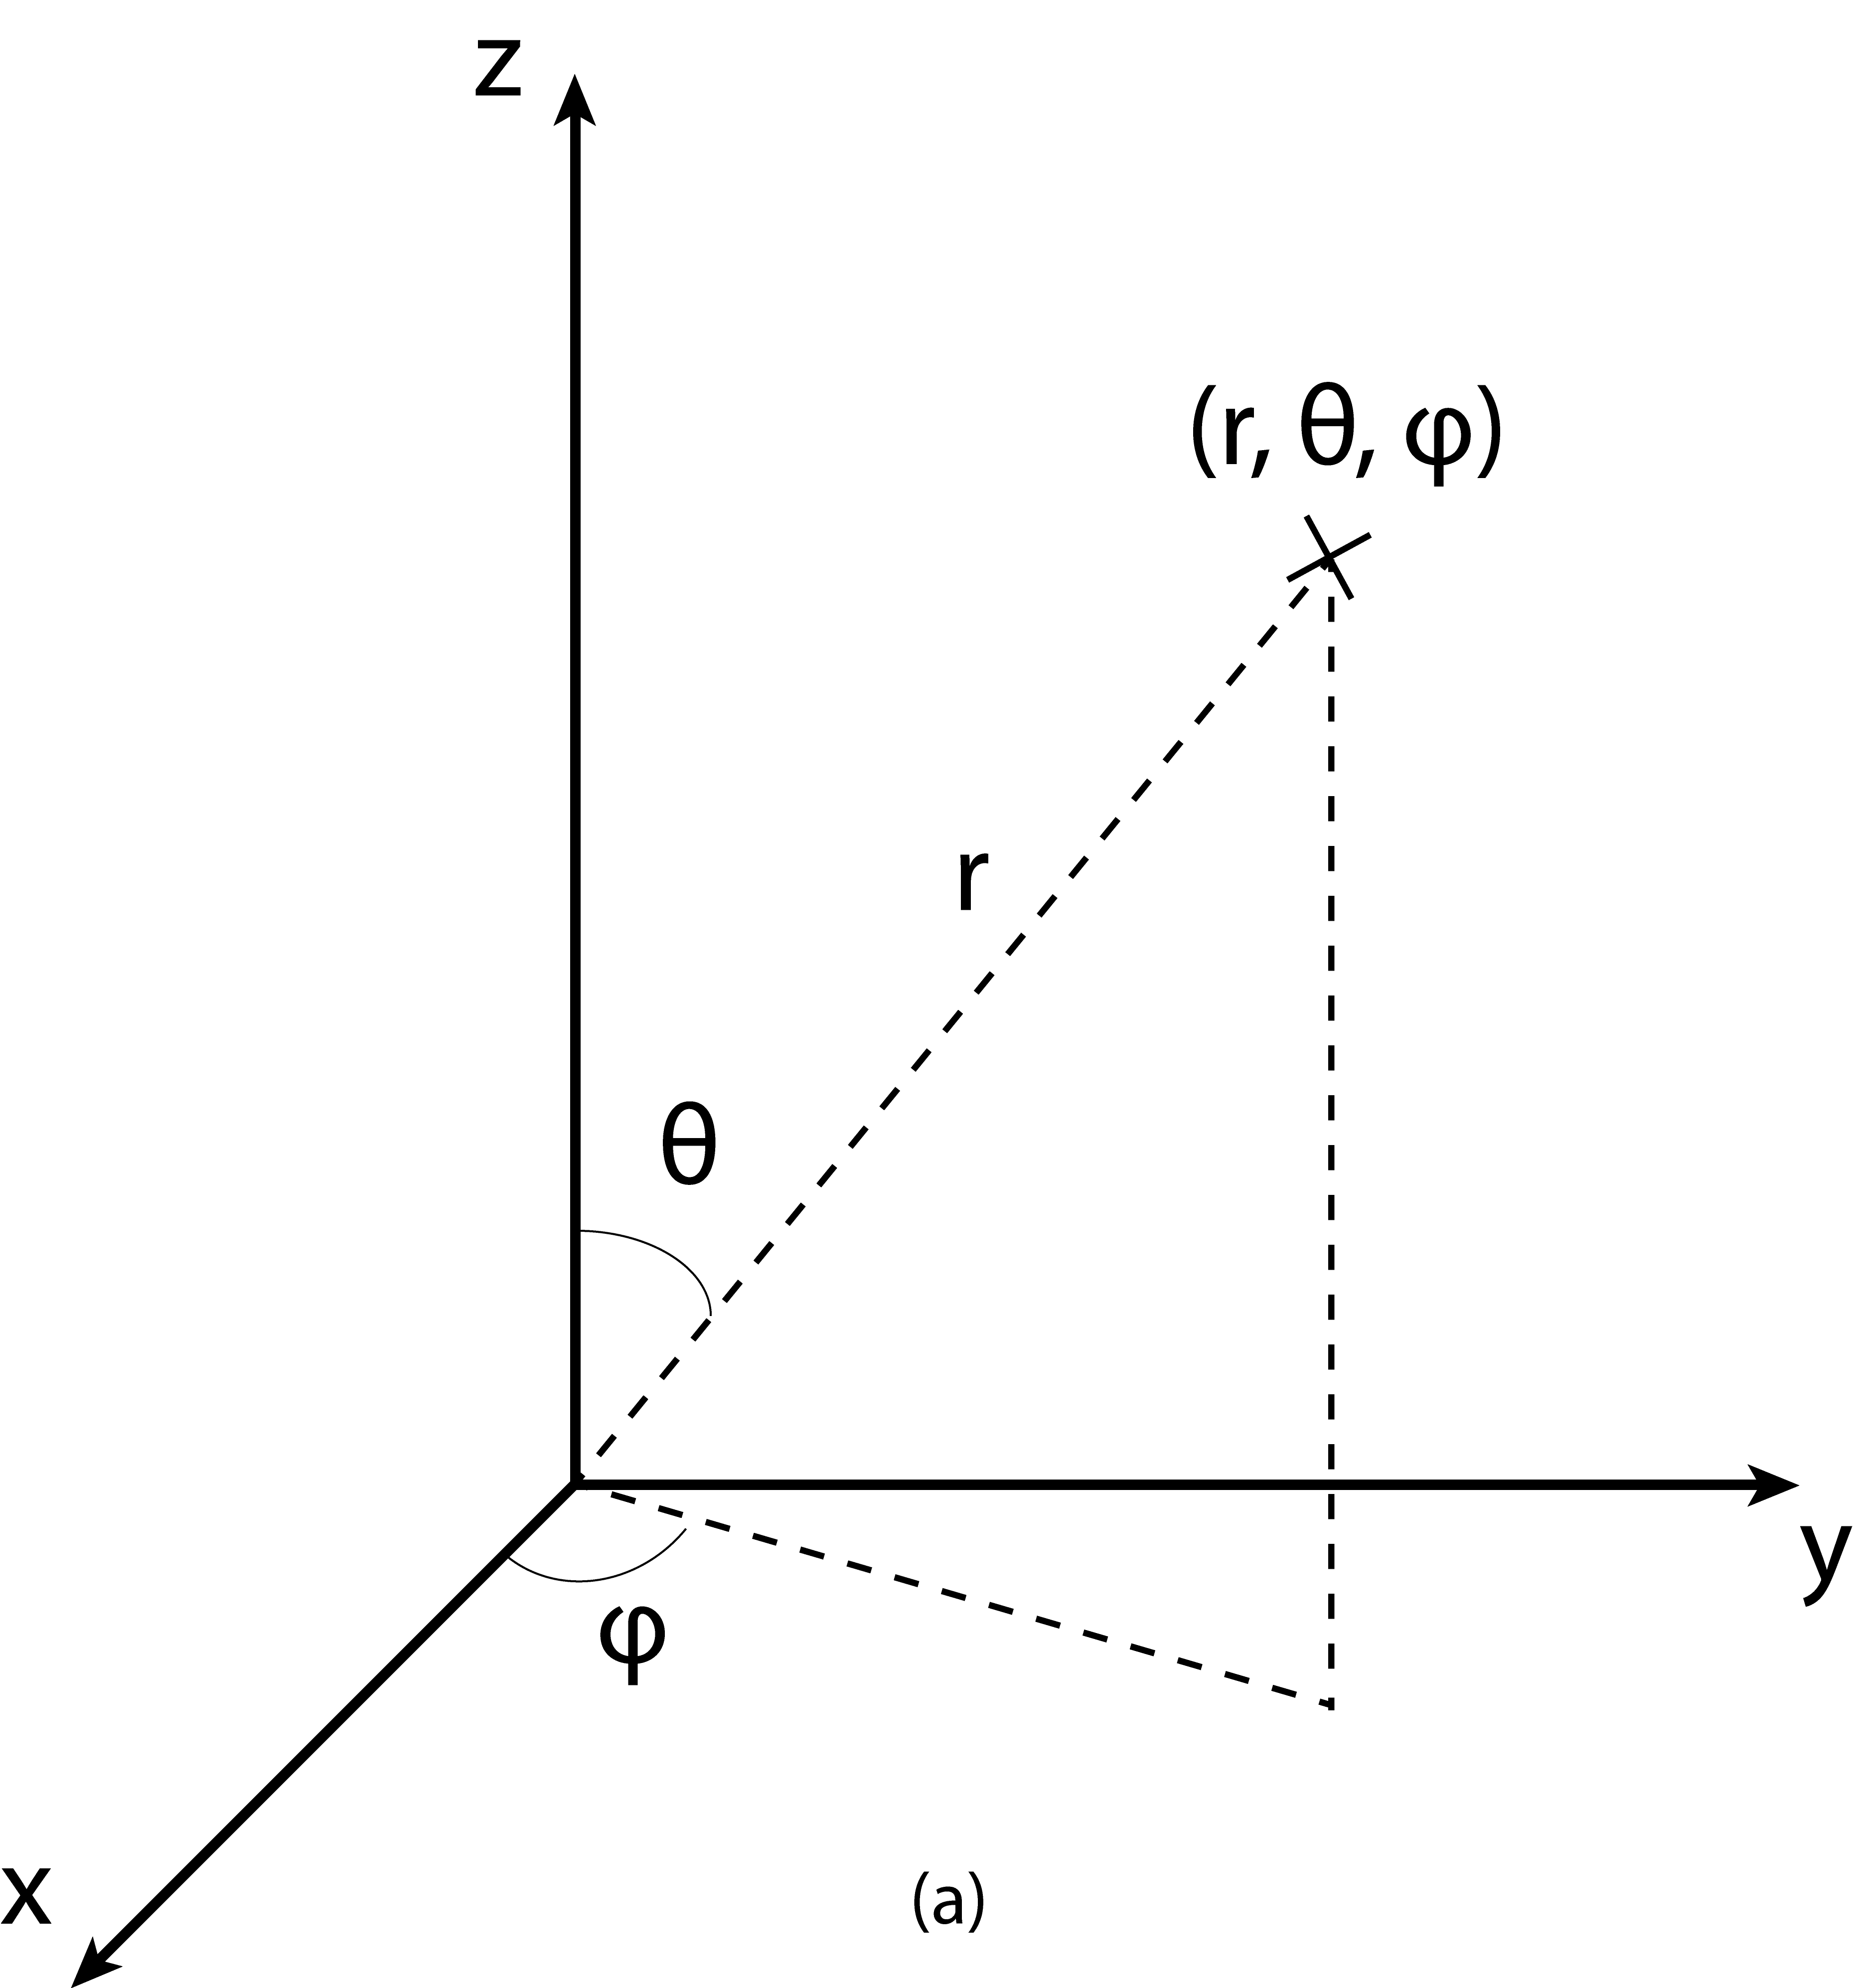
\includegraphics[scale=0.15]{gr-fig-3a.png}
	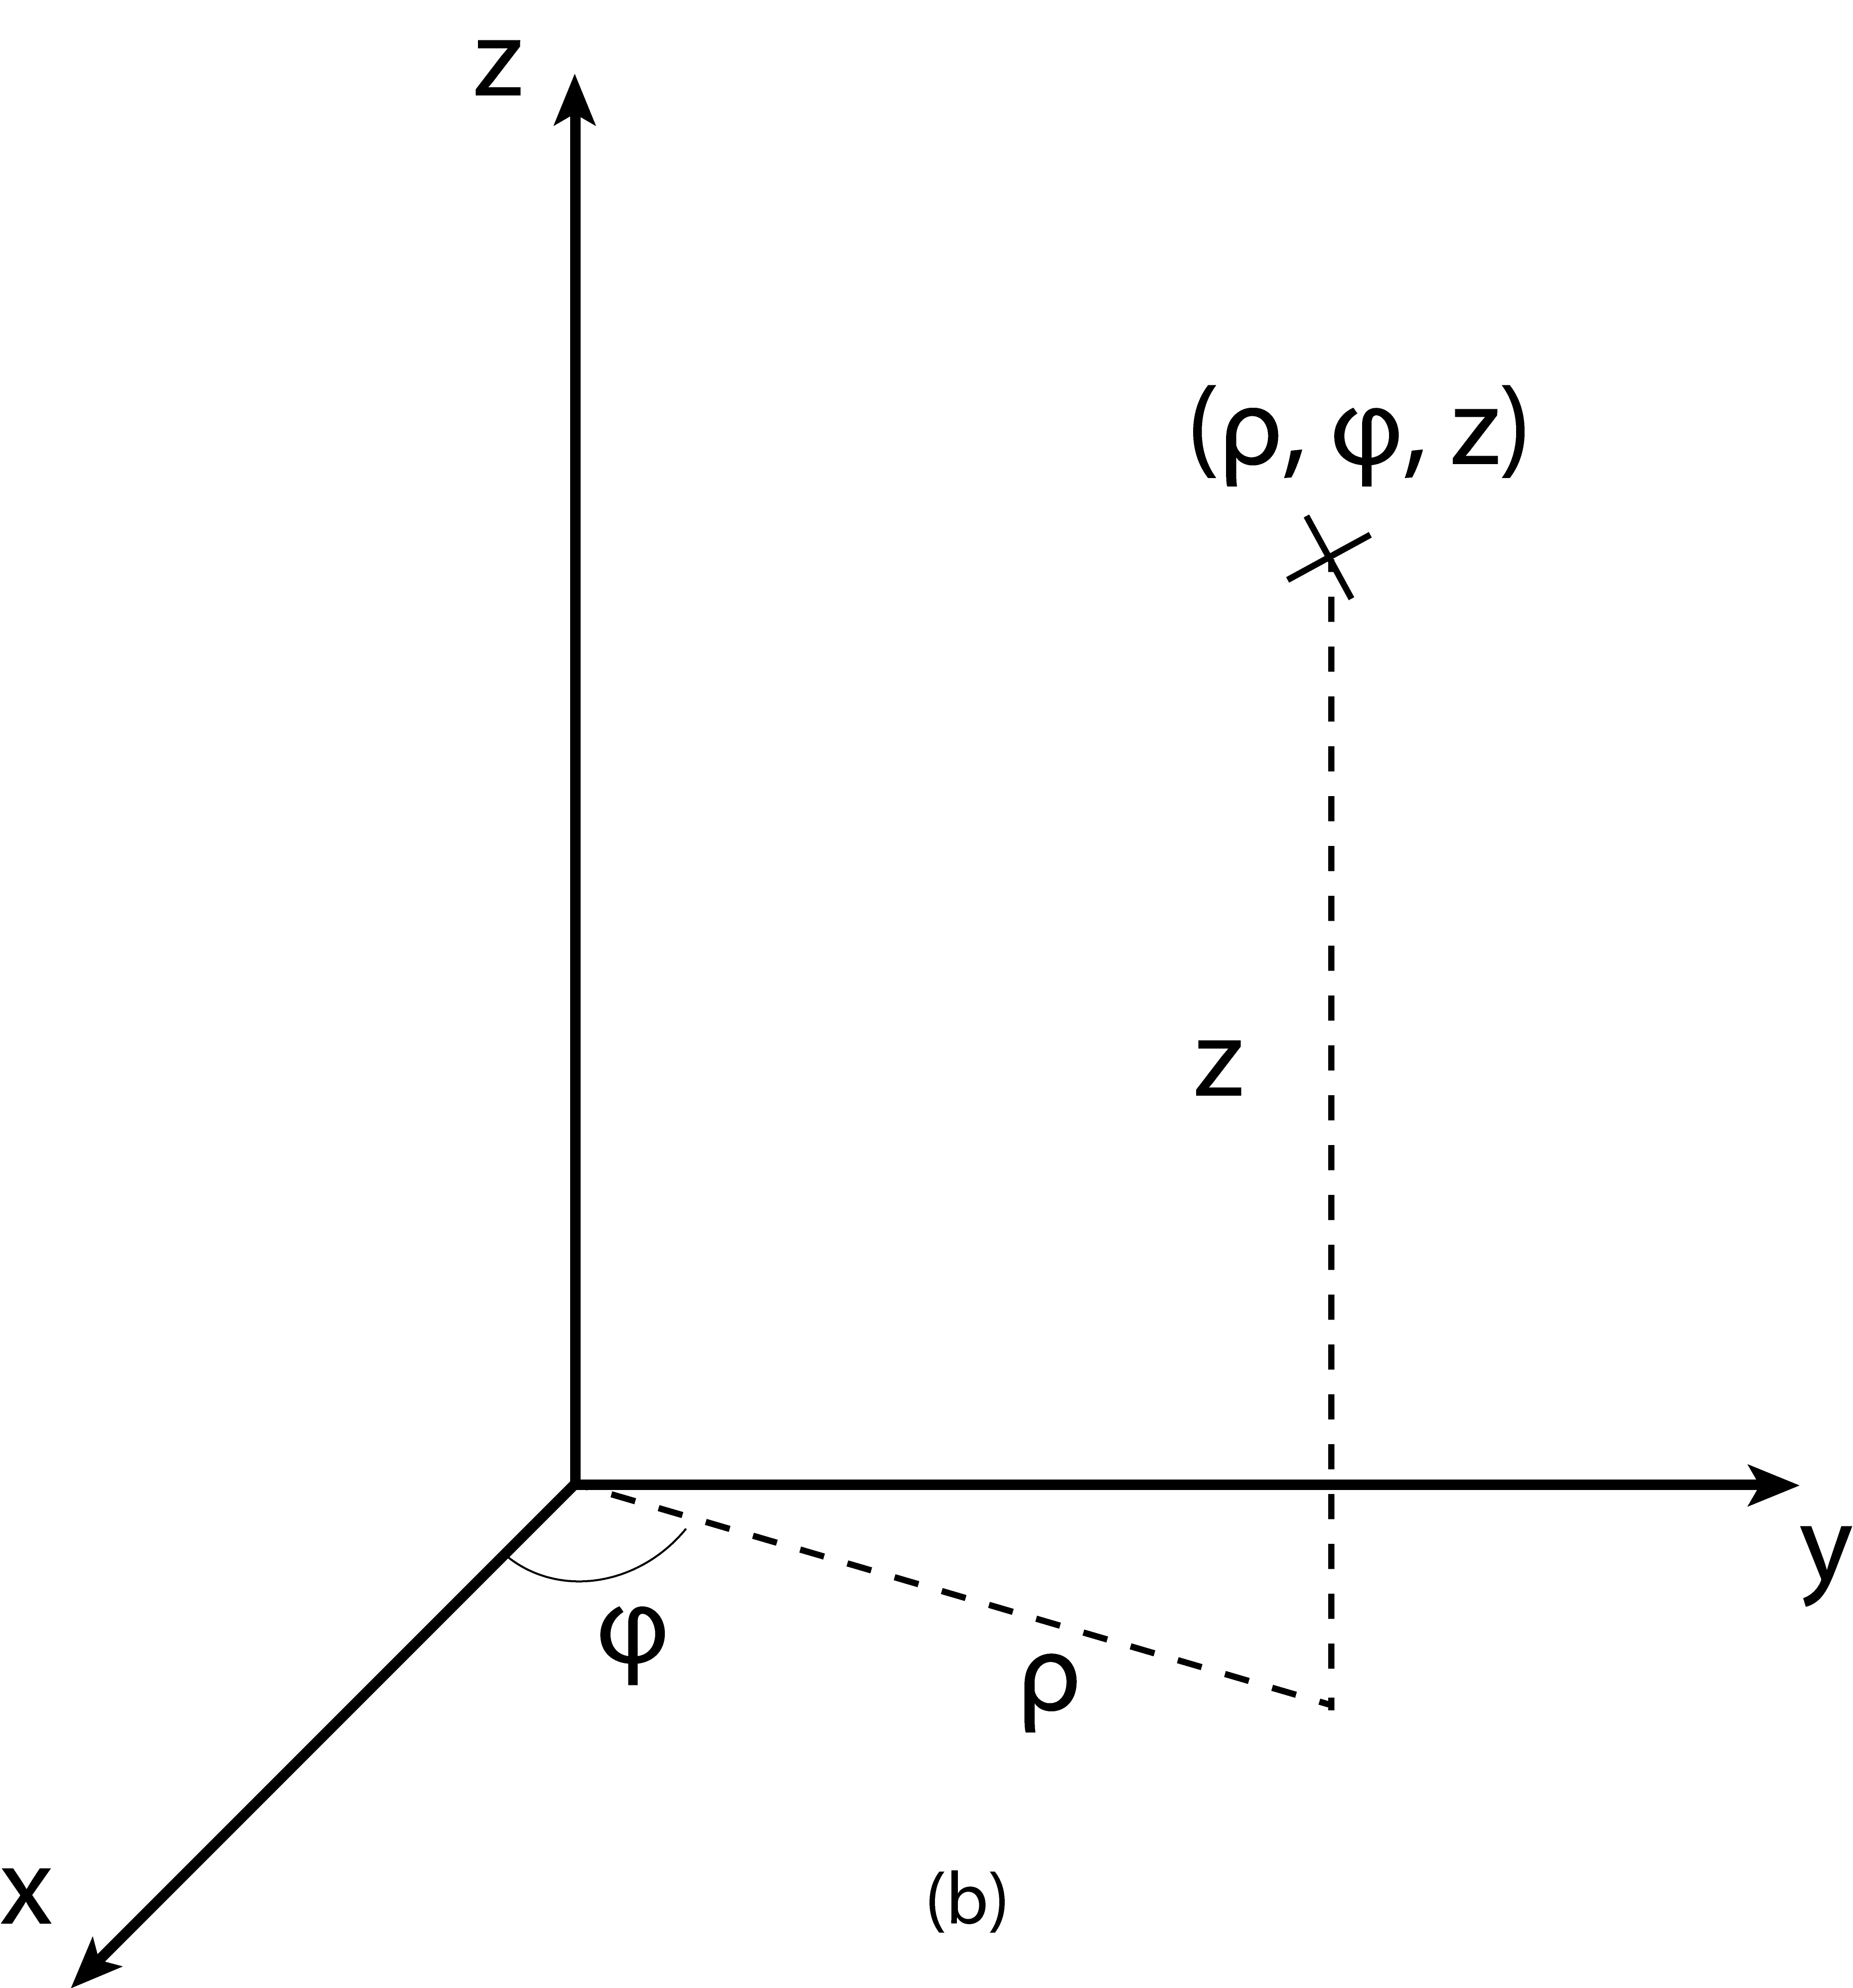
\includegraphics[scale=0.15]{gr-fig-3b.png}
	\caption{(a) Spherical coordinates, (b) Cylindrical coordinates}
\end{figure}
The \textbf{volume element} is given by
\begin{align*}
dV = dx\,dy\,dz = r^2\sin\theta\,dr\,d\theta\,d\phi.
\end{align*}
Consider a sphere of radius $R$. The \textbf{area element} is given by
\begin{align*}
dA = R\,d\theta\,d\phi.
\end{align*}
In \textbf{cylindrical coordinates},
\begin{align*}
x &= \rho\cos\phi\\
y &= \rho\sin\phi\\
z &= z
\end{align*}
and the inversion relations are
\begin{align*}
\rho &= \sqrt{x^2+y^2}\\
z &= z\\
\phi &= \tan^{-1}\left(\frac{y}{x}\right) 
\end{align*}
The \textbf{volume element} is given by
\begin{align*}
dV = r\,dt\,dz\,d\phi.
\end{align*}
Consider a cylinder of radius $R$, the \textbf{area element} is given by 
\begin{align*}
dA = R\,dz\,d\phi.
\end{align*}
The purpose of having the area and volume elements is so that we could integrate over regions, parameterized in spherical or cylindrical coordinates. While it seems like these quantities appear out of the blue, there is a general procedure to find them, given any arbitrary coordinate system. This ``procedure'' is called the \textbf{Jacobian}, which essentially gives the scaling factor as we move from one coordinate system into another. We know that the area element in polar coordinate is $dA = r\,dr\,d\theta$. We can see this is true, using the Jacobian. First, the Jacobian matrix, which is characteristic of a transformation from coordinate system $u^i$ into $u^{j'}$ is defined as
\begin{align*}
\boxed{[U^{j'}_{i}] = \left[ \frac{\partial u^{j'}}{\partial u^{i}} \right] = 
\begin{pmatrix}
\frac{\partial u^1}{\partial u^{1'}} & \dots & \frac{\partial u^1}{\partial u^{n'}}\\
\vdots & \ddots & \vdots\\
\frac{\partial u^n}{\partial u^{1'}} & \dots & \frac{\partial u^n}{\partial u^{n'}}
\end{pmatrix}}
\end{align*}
Note that $i$ and $j'$ are indices, not powers. Now, the general \textbf{scaling factor} is defined by the following equality
\begin{align*}
\Aboxed{N = du^{1'}\,du^{2'}\dots\,du^{n'} = \left| \det([U^{j}_{i}])\right| \,du^1\,du^2\dots\,du^{n}}
\end{align*}
\begin{exmp}
The scaling factor as we move from 2-dimensional Cartesian coordinates into polar coordinates is
\begin{align*}
N = \det\begin{pmatrix}
\frac{\partial x}{\partial r} & \frac{\partial x}{\partial \theta}\\
\frac{\partial y}{\partial r} & \frac{\partial y}{\partial \theta}
\end{pmatrix}
=
\det\begin{pmatrix}
\cos\theta & -r\sin\theta\\
\sin\theta & r\cos\theta
\end{pmatrix}
=
r.
\end{align*}
So, the area element is $dA = dx\,dy = rdr\,d\theta$, as expected. 
\end{exmp}
\begin{exmp}
We can try repeating the same procedure to get the volume element for spherical coordinates, which we have said before to be $dV = r^2\sin\theta\,dr\,d\theta\,d\phi$. First, define the Jacobian matrix:
\begin{align*}
[U^{j'}_{i}] = \begin{pmatrix}
\frac{\partial x}{\partial r} & \frac{\partial x}{\partial \theta} & \frac{\partial x}{\partial \phi}\\
\frac{\partial y}{\partial r} & \frac{\partial y}{\partial \theta} & \frac{\partial y}{\partial \phi}\\
\frac{\partial z}{\partial r} & \frac{\partial z}{\partial \theta} & \frac{\partial z}{\partial \phi}
\end{pmatrix}
=
\begin{pmatrix}
\sin\theta\cos\phi & r\cos\theta\cos\phi & -r\sin\theta\sin\phi \\
\sin\theta\sin\phi & r\cos\theta\sin\phi & r\sin\theta\cos\phi \\
\cos\theta & -r\sin\theta & 0
\end{pmatrix}
\end{align*}
After some bookkeeping-type rearrangements and computation, we find that
\begin{align*}
N = \left|\det[U^{j'}_{i}]\right|= r^2\sin\theta,
\end{align*}
as expected. As a check, we can integrate this volume element over a region defined by $x^2+y^2+z^2 = R^2$ to find its volume
\begin{align*}
\int_{0}^{R}\int_{0}^{\pi}\int_{0}^{2\pi}r^2\sin\theta\,dr\,d\theta\,d\phi = \frac{4}{3}\pi R^3,
\end{align*}
which is not surprisingly the volume of the sphere of radius $R$. 
\end{exmp}
\newpage

\section{Flat 3-dimensional space}
Flat, or ``Euclidean'' space are spaces with \textbf{no curvature}. For instance, a flat sheet of paper in $\mathbb{R}^3$ is considered ``flat'' while the surface of a sphere embedded in $\mathbb{R}^3$ is considered curved space. There should also be a distinction between a sphere in $\mathbb{R}^3$ and a sphere \textbf{embedded} into $\mathbb{R}^3$. The former case is simply some subset of flat 3-dimensional space, so it is considered flat. But in the latter case, the sphere is a curved 2-dimensional space, although it lives in flat 3-dimensional space.\\

Our goal in this section is to see how  we can use any arbitrary coordinate system, which specify points in 3-dimensions as an intersection of 3 surfaces. For instance, in Cartesian coordinates, a point ($a^1,a^2,a^3$) is specified by 3 planes: $x = a^1$, $y=a^2$, and $z=a^3$. In spherical coordinates, a point is specified by intersecting a sphere of radius $r$, a cone with azimuth angle $\theta$, and a plane of constant $\phi$. In cylindrical coordinates, a point is specified by intersecting a cylinder of radius $\rho$, vertical plane of constant $\phi$ to the $x-$axis, and the horizontal plane of constant $z$.
\begin{figure}[h!]
	\centering
	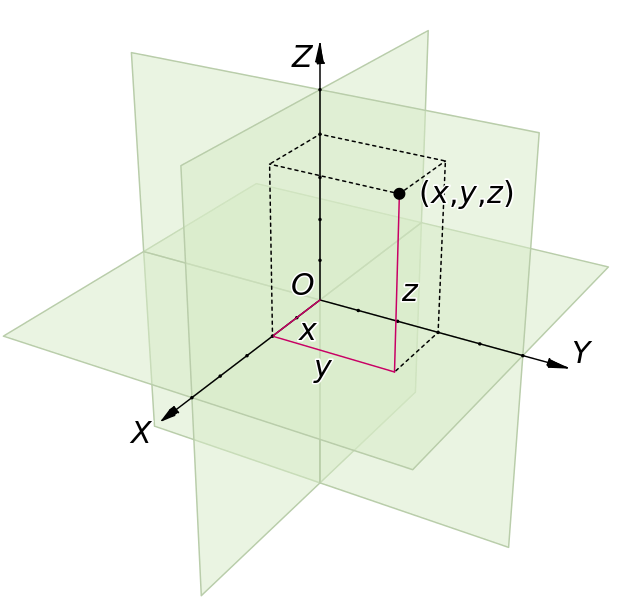
\includegraphics[scale=0.2]{gr-fig-4a.png}
	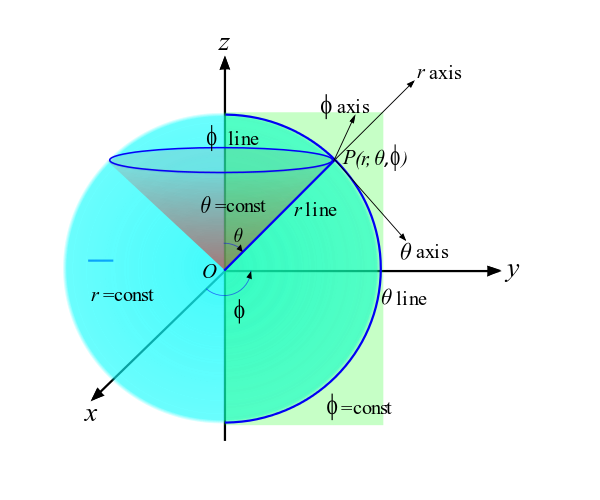
\includegraphics[scale=0.25]{gr-fig-4b.png}
	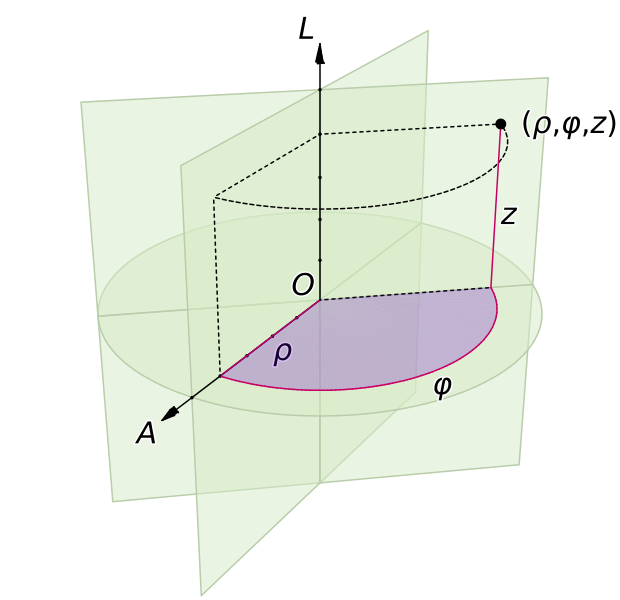
\includegraphics[scale=0.2]{gr-fig-4c.png}
	\caption{(a) Three intersecting (mutually distinct) planes define a point in Cartesian coordinates (\href{https://en.wikipedia.org/wiki/Cartesian_coordinate_system}{source}), (b) Three intersecting surfaces (a cone, a sphere, and a plane) defining a point in spherical coordinates (\href{https://en.wikipedia.org/wiki/Curvilinear_coordinates}{source}), and (c) Three intersecting surfaces (two planes and a cylinder) defining a point in cylindrical coordinates (\href{https://en.wikipedia.org/wiki/Cylindrical_coordinate_system}{source}).}
\end{figure}

\subsection{Curvilinear coordinates}
Curvilinear coordinates are an arbitrary coordinate system in Euclidean space where coordinate lines can be curved (hence curvilinear). Note that although coordinate lines can be curvy, the space is still flat. We can call $(u,v,w)$ our arbitrary coordinates, which specify a point $(a^1,a^2,a^3)$ by intersecting three surfaces: $u = a^1$, $v=a^2$, $w=a^3$. Let let relations between $(u,v,w)$ and $(x,y,z)$ be established as
\begin{align*}
u &= u(x,y,z); \text{ } x = x(u,v,w)\\
v &= v(x,y,z); \text{ } y = y(u,v,w)\\
w &= w(x,y,z); \text{ } z = z(u,v,w)
\end{align*} 
\begin{figure}[h!]
	\centering
	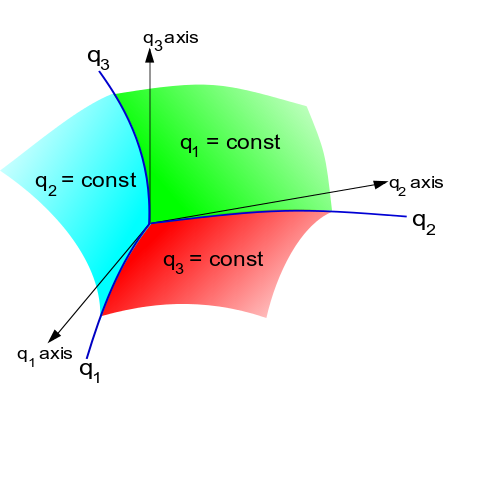
\includegraphics[scale=0.5]{gr-fig-5.png}
	\caption{In curvilinear coordinates, a point is defined by the intersection of level surfaces (\href{https://en.wikipedia.org/wiki/Curvilinear_coordinates}{source}).}
\end{figure}

\subsection{Basis vectors}
\subsection{Natural basis}
Next, since we want to be able to describe vectors using arbitrary curvilinear coordinates, we need to know a \textbf{basis set} of vectors that span the space. In Cartesian coordinates, such a basis set is $\{\hat{i},\hat{j},\hat{k}\}$. Similarly, we want to find a set $\{\vec{e}_u, \vec{e}_v, \vec{e}_w\}$ that would give a basis for an arbitrary curvilinear coordinate system. The way we obtain this set is the same as how we obtain $\{\hat{i}, \hat{j}\, \hat{k}\}$ from Cartesian coordinates. We notice that $\hat{i}$ is a vector that follows the change in the $x$-direction with $y$ and $z$ fixed, i.e., $\hat{i}$ is a tangent vector to a vector $\vec{r}$ along the change in $x$. Hence
\begin{align*}
\hat{i} = \frac{\partial \vec{r}}{\partial x}.
\end{align*}
Likewise, $\hat{j} = \frac{\partial \vec{r}}{\partial y}$, and $\hat{k} = \frac{\partial \vec{r}}{\partial z}$. By analogy, we can define the set $\{ \vec{e}_u, \vec{e}_v, \vec{e}_w\}$ with
\begin{align*}
\vec{e}_u = \frac{\partial \vec{r}}{\partial u}, \text{ } \vec{e}_v = \frac{\partial \vec{r}}{\partial v}, \text{ } \vec{e}_w = \frac{\partial \vec{r}}{\partial w},
\end{align*}
In general, given a coordinate system with $(u^1,u^2,\dots,u^n)$, we can define a \textbf{natural basis set} by letting
\begin{align*}
\Aboxed{\vec{e}_{u^i} = \frac{\partial \vec{r}}{\partial u^i}}
\end{align*}
where $i = 0,1,2,\dots,n$ are indices. Note that the set $\{\vec{e}_{u^i} \}$ need not be orthogonal. The only requirement is that they have to be linearly independent and span the space. We also note that they need not be unit vectors. It is possible to make a basis set of only unit vectors by letting
\begin{align*}
\hat{e}_u = \frac{\vec{e}_u}{\vert\vert \vec{e}_u\vert\vert},
\end{align*}
but we will see that this definition is not so useful in general relativity. A question one might ask is: ``What is \textbf{natural} about this basis set?'' The answer, unfortunately, will be provided in the following sections, where we will discuss how they give rise to the \textbf{metric tensor}.\\

We will often use $\{\hat{i}, \hat{j}, \hat{k} \}$ as a reference basis, i.e., we can express $\{\vec{e}_u, \vec{e}_v ,\vec{e}_w\}$ in terms of these:
\begin{align*}
\vec{\epsilon_u} = (e_u)_x\hat{i} + (e_u)_y\hat{j} + (e_u)_z\hat{k}.
\end{align*}
\begin{exmp}
We can look at the basis set for the spherical coordinate system, $\{\vec{e}_r, \vec{e}_\theta, \vec{e}_\phi \}$. First, let the coordinates $(u,v,w)$ be $(r,\theta,\phi)$, the spherical coordinates. A vector $\vec{r}$, expressed in spherical coordinates, has the form:
\begin{align*}
\vec{r} = 
\begin{pmatrix}
r\sin\theta\cos\phi\\
r\sin\theta\sin\phi\\
r\cos\theta
\end{pmatrix},
\end{align*}
where $r \geq 0$, $0 \leq \theta \leq \pi$, and $0 \leq \phi \leq 2\pi$. To obtain the basis vectors, we simply take $\partial \vec{r}/\partial r$, $\partial \vec{r}/\partial \theta$, and $\partial \vec{r}/\partial \phi$. We expect that our resulting vectors should form the column vectors of the Jacobian matrix $[U^{j'}_i]$, which, as we have discussed previously, has the following form:
\begin{align*}
[U^{j'}_i] = 
\begin{pmatrix}
\sin\theta\cos\phi & r\cos\theta\cos\phi & -r\sin\theta\sin\phi \\
\sin\theta\sin\phi & r\cos\theta\sin\phi & r\sin\theta\cos\phi \\
\cos\theta & -r\sin\theta & 0
\end{pmatrix}.
\end{align*}
What we're doing now, in terms of linear algebra, is essentially constructing $[U^{j'}_i]$ - the change-of-basis matrix. Let's see if our described procedure works:
\begin{align*}
\vec{e}_r &= \frac{\partial \vec{r}}{\partial r} = \begin{pmatrix}
\sin\theta\cos\phi\\
\sin\theta\sin\phi\\
\cos\theta
\end{pmatrix}\\
\vec{e}_\theta &= \frac{\partial \vec{r}}{\partial \theta} = 
\begin{pmatrix}
r\cos\theta\cos\phi\\
r\cos\theta\sin\phi\\
-r\sin\theta
\end{pmatrix}\\
\vec{e}_\phi &= \frac{\partial \vec{r}}{\partial \phi}=
\begin{pmatrix}
-r\sin\theta\sin\phi\\
r\sin\theta\cos\phi\\
0
\end{pmatrix}
\end{align*} 
Not surprisingly,
\begin{align*}
[U^{j'}_i] = 
\begin{pmatrix}
\sin\theta\cos\phi & r\cos\theta\cos\phi & -r\sin\theta\sin\phi \\
\sin\theta\sin\phi & r\cos\theta\sin\phi & r\sin\theta\cos\phi \\
\cos\theta & -r\sin\theta & 0
\end{pmatrix}
=
\left( \vec{e}_r \vert \vec{e}_\theta \vert \vec{e}_\phi \right).
\end{align*}
Next, we can check if ${\vec{e}_r, \vec{e}_\theta, \vec{e}_\phi}$ is mutually-perpendicular set. (Note that I avoid the word ``orthogonal'' here, since it carries different meanings in physics and in linear algebra). We can also check whether the three vectors are unit vectors. It suffices to take the dot products of ${\vec{e}_r, \vec{e}_\theta, \vec{e}_\phi}$ among themselves:
\begin{align*}
\vec{e}_r\cdot\vec{e}_r &= \sin^2\theta(\cos^2\phi + \sin^2\phi) + \cos^2\theta = 1\\
\vec{e}_r\cdot\vec{e}_\theta &= r\cos^2\phi\sin\theta\cos\theta + r\sin^2\phi\sin\theta\cos\theta - r\sin\theta\cos\theta = 0\\
\vec{e}_r\cdot\vec{e}_\phi &= -r\sin^2\theta\sin\phi\cos\phi + r\sin^2\theta\sin\phi\cos\phi = 0\\ 
\vec{e}_\theta\cdot\vec{e}_\theta &= r^2\cos^2\phi\cos^2\theta + r^2\cos^2\phi\sin^2\theta + r^2\sin^2\theta = r^2\\ 
\vec{e}_\theta\cdot\vec{e}_\phi &= 0 \\
\vec{e}_\phi\cdot\vec{e}_\phi &= r^2\sin^2\phi\sin^2\theta + r^2\sin^2\theta\cos^2\phi = r^2\sin^2\theta.
\end{align*}
We notice that all dot products of cross-coordinates result in 0, which means the basis vectors we found are mutually perpendicular (we can also see this fat geometrically, based on how the spherical coordinates are defined). But we also find that these basis vectors are not unit vectors, since their norms are not necessarily 1:
\begin{align*}
\vert\vert \vec{e}_r \vert\vert &= 1\\
\vert\vert \vec{e}_\theta \vert\vert &= r\\
\vert\vert \vec{e}_\phi \vert\vert &= r\sin\theta.
\end{align*}
\end{exmp}
\subsection{Dual basis}
The procedure we have described in the previous subsection allows us to find a \textbf{natural basis} set of vectors for a coordinate system. However, basis sets are not unique. In this section, we look at an alternative basis set of vectors, called the \textbf{dual basis} set, denoted $\{ \vec{e}^{\,u}, \vec{e}^{\,v}, \vec{e}^{\,w},\dots \}$. Instead of deriving these from the finding the tangent vectors, we find the normal of surfaces of constant $u,v,w,\dots$\\

Recall that the \textbf{gradient} operator $\vec{\nabla}$, when applied to a scalar field $f$, gives the normal vectors to surfaces of constant $f$. Since curvilinear coordinates are given by coordinate lines where $u,v$, or $w$ is constant, we can let
\begin{align*}
\vec{e}^{\,u} &= \vec{\nabla}u\\
\vec{e}^{\,v} &= \vec{\nabla}v\\
\vec{e}^{\,w} &= \vec{\nabla}w,
\end{align*}  
and so on, where $\vec{e}^{\,u}$ is a normal vector to the surface of constant $u$. Or more generally, 
\begin{align*}
\boxed{\vec{e}^{\,u^i} = \vec{\nabla}u^i}
\end{align*} 
Now, we might wonder what the dual basis in Cartesian coordinates is. It turns out the dual and natural basis sets in Cartesian coordinates are the same:
\begin{align*}
\vec{e}^{\,x} &= \vec{\nabla}x=(1,0,0)^\top=\hat{i} = \vec{e}_x \\
\vec{e}^{\,y} &= \vec{\nabla}y=(0,1,0)^\top=\hat{j} = \vec{e}_y \\
\vec{e}^{\,z} &= \vec{\nabla}z=(0,1,0)^\top=\hat{k} = \vec{e}_z.
\end{align*}
There's actually no magic behind this ``coincidence.'' The reason the basis sets are the same is simply that the direction of increasing/decreasing $x$ is the same as the normal vector to the surface of constant $x$, i.e., the $yz$-plane. 
\begin{align*}
\text{insert figure 6 here!!!}
\end{align*}
However, we suspect that this is not the case in general curvilinear coordinates, since the direction of increasing $u$, for instance, should not necessarily be the same as the normal vector to the surface of constant $u$, as illustrated here:
\begin{align*}
\text{insert figure 7 here!!!}
\end{align*}
\begin{exmp}
We can look at the dual basis set for the spherical coordinate system. Based on what we have established so far, we can compute the dual basis set, using the inverse relations $(x,y,z) \rightarrow (r,\theta,\phi)$.
\begin{align*}
\vec{e}^{\,r} &= \vec{\nabla}r = \vec{\nabla}(x^2+y^2+z^2)^{1/2} = (x^2+y^2+z^2)^{-1/2}\begin{pmatrix}x\\y\\z\end{pmatrix} = \begin{pmatrix}\sin\theta\cos\phi\\ \sin\theta\sin\phi\\ \cos\theta\end{pmatrix}.
\end{align*}
Tedious and painstaking computations give us the other two vectors:
\begin{align*}
\vec{e}^{\,\theta} &= \frac{1}{r}\begin{pmatrix} \cos\theta\cos\phi \\ \cos\theta\sin\phi \\ -\sin\theta \end{pmatrix}\\
\vec{e}^{\,\phi} &= \frac{1}{r}\begin{pmatrix} -\frac{\sin\phi}{\sin\theta} \\ \frac{\cos\phi}{\sin\theta} \\ 0\end{pmatrix}
\end{align*}
We can readily compare $\{ \vec{e}^{\,r}, \vec{e}^{\,\theta}, \vec{e}^{\,\phi} \}$ to $\{ \vec{e}_{r}, \vec{e}_\theta, \vec{e}_\phi \}$ and find that while $\vec{e}^{\,r} = \vec{e}_{r}$, $\vec{e}^{\,\theta} \neq \vec{e}_{\theta}$ and $\vec{e}^{\,\phi} \neq \vec{e}_{\phi}$.
\end{exmp}
\begin{exmp}
Let's consider a non-familiar case of paraboloidal surfaces $(u,v,w)$, a non-orthogonal set, where
\begin{align*}
x &= u+v\\y&=u-v\\z&=2uv+w,
\end{align*}
which gives the inverse relations
\begin{align*}
u&=\frac{1}{2}(x+y)\\
v&=\frac{1}{2}(x-y)\\
w&=z-\frac{1}{2}(x^2-y^2).
\end{align*}
Let $\vec{r} = (x,y,z)^\top = (u+v, u-v, 2uv + w)^\top$. We first obtain the natural basis set:
\begin{align*}
\vec{e}_u &= \frac{\partial \vec{r}}{\partial u} = (1,1,2v)^\top \\
\vec{e}_v &= \frac{\partial \vec{r}}{\partial v} = (1,1,2u)^\top \\
\vec{e}_w &= \frac{\partial \vec{r}}{\partial w} = (0,0,1)^\top, 
\end{align*}
which is an mutually perpendicular set, by inspection (i.e., all cross-dot product terms are zero). Next, we obtain the dual basis set:
\begin{align*}
\vec{e}^{\,u} &= \vec{\nabla}u = \frac{1}{2}\vec{\nabla}(x+y) = \left( \frac{1}{2}, \frac{1}{2},0\right) ^\top\\
\vec{e}^{\,v} &= \vec{\nabla}v = \frac{1}{2}\vec{\nabla}(x-y) = \left( \frac{1}{2}, -\frac{1}{2},0\right) ^\top\\
\vec{e}^{\,w} &= \vec{\nabla}w = \vec{\nabla}\left( z-\frac{1}{2}(x^2-y^2)\right)  = (-x,y,1)^\top = (-u-v,u-v,1)^\top\\
\end{align*}
But notice that we get non-zero cross-dot product terms:
\begin{align*}
\vec{e}^{\,u}\cdot\vec{e}^{\,w} &= -v \\
\vec{e}^{\,u}\cdot\vec{e}^{\,v} &= 0 \\
\vec{e}^{\,v}\cdot\vec{e}^{\,w} &= -u. 
\end{align*}
The reason for observing what value the dot products between basis vectors are will become clear when we talk about the \textbf{metric tensor} in the next subsections.
\end{exmp}
\subsection{Contravariant and covariant vectors}
\subsubsection{The suffix notation (vector calculus)}
In general coordinate systems, there can be many more than three coordinates, and it can be burdensome to keep track of different letters representing these coordinates, especially if they don't follow a convention. It is convenient to change our notation from ``letter-based'' to ``index-based.'' For example, instead of using $(u,v,w)$ as coordinates, we will now use $(u^1,u^2,u^3)$, for $i=1,2,3$. Note that we are using upper indices here. As we will discuss soon, upper and lower indices have different meanings. \\

Similarly, our notation for basis vectors also change. For the natural basis, we ``code'' $\{ \vec{e}_u, \vec{e}_v, \vec{e}_w \}$ as $\{\vec{e}_i \}$, where $i=1,2,3$. For the dual basis, we ``code'' $\{ \vec{e}^{\,u},\vec{e}^{\,v},\vec{e}^{\,w} \}$ as $\{ \vec{e}^{\,i} \}$ for $i=1,2,3$. Our vector notation also changes as a result, but there are additional rules. Let vector $\vec{\lambda}$ be given. In the \textbf{natural basis}, the components of $\lambda$ is written with \textbf{upper} indices,
\begin{align*}
\vec{\lambda} = \lambda^1\vec{e}_1 + \lambda^2\vec{e}_2 + \lambda^3\vec{e}_3 = \sum_{i=1}^{3}\lambda^1\vec{e}_i.
\end{align*} 
and in the \textbf{dual basis}, we use \textbf{lower} indices for the components:
\begin{align*}
\vec{\lambda} = \lambda_1\vec{e}^{\,1} + \lambda_2\vec{e}^{\,2} + \lambda_3\vec{e}^{\,3} = \sum_{i=1}^{3}\lambda_i\vec{e}^{\,i}
\end{align*}

\subsubsection{The Einstein summation notation}
We shall make another ``leap in notation'' as we introduce the Einstein summation convention:
\begin{align*}
\boxed{\text{Any index that appears once up and once down is automatically summed}}
\end{align*}
For example, from now on, we will write $\vec{\lambda}$ as:
\begin{align*}
{\vec{\lambda}} = \sum_{i=1}^{3}\lambda^i\vec{e}_i = {\lambda^i\vec{e}_i}
\end{align*}
Note that this summation convention removes us from indicating the minimum and maximum values for our indices, which allows us to keep the mathematics as applicable to any n-dimensional system as possible. We should also notice that indices can be exchangeable, especially in summed situations. For example, 
\begin{align*}
\boxed{a^ib_i = a^jb_j = \dots = \sum_{n=1}^{N}a^nb_n}
\end{align*}
Keep in mind that $a_ib_i$ does not make sense in the Einstein convention. If we want to denote a sum, we have to specify the range of $i$ as follows:
\begin{align*}
\sum_{i=n}^{N}a_ib_i.
\end{align*} 
Likewise, $a_ib^ic^i$ is not defined either. Remember that only ``1 up index, 1 down index'' is allowed. Finally, it is widely agreed upon that certain letters are reserved for some specific cases. For instance, $i,j,k,l,\dots = 1,2,3$ are reserved for 3-dimensional space. We use Greek characters $\mu, \nu, \alpha, \beta,\dots = 0,1,2,3$ for 4-dimensional spacetime, $A,B,C,\dots = 1,2$ for 2-dimensional spaces, and $a,b,c,\dots = 1,2,\dots,N$ for N-dimensional manifolds. 

\subsubsection{Contravariant and covariant vectors}
\begin{figure}[h!]
	\centering
	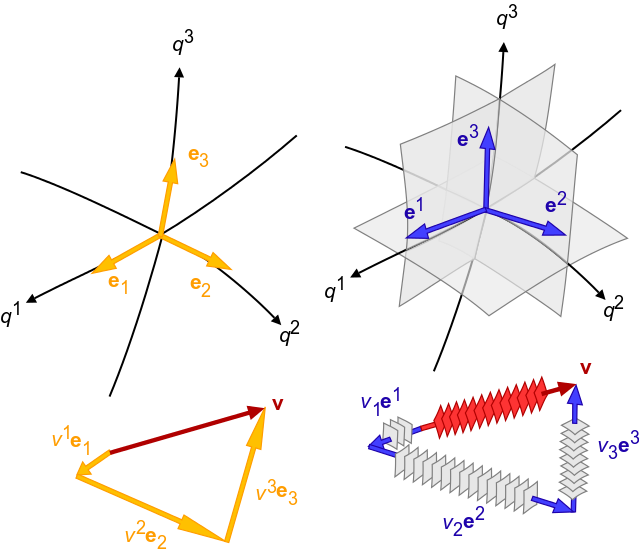
\includegraphics[scale=0.3]{gr-fig-add1.png}
	\caption*{\href{https://en.wikipedia.org/wiki/Covariance_and_contravariance_of_vectors}{Source}}
\end{figure}
Earlier, we have established that any vector $\vec{\lambda}$ can be written in two ``upper-lower index'' ways, depending on whether we are using the natural or the dual basis set:
\begin{align*}
\vec{\lambda} = \lambda^i\vec{e}_i = \lambda_i\vec{e}^{\,i}.
\end{align*}
We shall now call $\lambda^i$ the \textbf{contravariant} components and $\lambda_i$ the \textbf{covariant} components. (Remember: ``co'' is ``low''). Contravariant vectors are simply vectors with contravariant components. Likewise, covariant vectors are vectors with covariant components. Later in this text, we will denote $\vec{\lambda}$ simply as $\lambda^i$ (contravariant vector) or $\lambda_i$ (covariant vector).\\

Putting together what we have established so far about index notation and Einstein summation convention, we can now look at the last interesting dot product: between a vector in the natural basis and one in the dual basis: $\vec{e}^{\,i}\cdot\vec{e}_j$. Before we proceed, keep in mind that this single expression ($\vec{e}^{\,i}\cdot\vec{e}_j$) represents 9 different objects because there is not summation here ($i$ is not necessarily $j$ and $i,j=1,2,3$). Now, recall the definitions of these vectors:
\begin{align*}
\vec{e}^{\,i} &= \vec{\nabla}u^i = \frac{\partial u^i}{\partial x}\hat{i} + \frac{\partial u^i}{\partial y}\hat{j} + \frac{\partial u^i}{\partial z}\hat{k}\\
\vec{e}_j &= \frac{\partial \vec{r}}{\partial u^j} = \frac{\partial x}{\partial u^j}\hat{i} + \frac{\partial y}{\partial u^j}\hat{j} + \frac{\partial z}{\partial u^j}\hat{k}
\end{align*}
Therefore,
\begin{align*}
\vec{e}^{\,i}\cdot\vec{e}_j = \frac{\partial u^i}{\partial x}\frac{\partial x}{\partial u^j} + \frac{\partial u^i}{\partial y}\frac{\partial y}{\partial u^j} + \frac{\partial u^i}{\partial z}\frac{\partial z}{\partial u^j}
\end{align*}
But notice that this is nothing but the chain rule, if we think about $u^i$ as $u^i(x,y,z)$. So,
\begin{align*}
\boxed{\vec{e}^{\,i}\cdot\vec{e}_j = \frac{\partial u^i}{\partial u^j}}
\end{align*}
But also notice that the $u^i$'s are independent variables, i.e.,
\[ \frac{\partial u^i}{\partial u^j} = 
\begin{cases*}
0 & \text{if $i \neq j$} \\
1 & \text{if $i = j$}
\end{cases*}\]
We can introduce a two-index object, the \textbf{Kronecker delta}, defined as
\[ \boxed{\delta^i_j = 
\begin{cases*}
	0 & \text{if $i \neq j$} \\
	1 & \text{if $i = j$}
\end{cases*}}\]
We obtain an elegant relation:
\begin{align*}
\boxed{\vec{e}^{\,i}\cdot\vec{e}_j = \delta^i_j}
\end{align*}
Again, keep in mind that this is not a single equation but rather 9. Six of which are $0=0$ and three $1=1$. We observe that for $u\neq v$, $\vec{e}^{\,u}\cdot\vec{e}_v = 0$, i.e., $\vec{e}^{\,u} \perp \vec{e}_v$, which makes sense, by definition: 
\begin{figure}[h!]
	\centering
	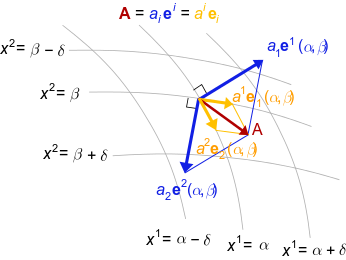
\includegraphics[scale=0.55]{gr-fig-8.png}
	\caption{The natural and basis vectors are defined such that $\vec{e}^{u}\cdot\vec{e}_v = \delta^u_v$. This is not so difficult to show mathematically (all simply follow form the definitions), but a figure can help visualize ``what's going on'' (\href{https://en.wikipedia.org/wiki/Covariance_and_contravariance_of_vectors}{source}).} 
\end{figure}
As a little aside, every time we see an two-index object, we should immediately think of a matrix. In matrix form, the Kronecker delta is our beloved identity matrix $I$:
\begin{align*}
[\delta^i_j] = 
\begin{pmatrix}
1 & 0 & 0\\
0 & 1 & 0\\
0 & 0 & 1
\end{pmatrix}
\end{align*}
What about the dot (or inner) products of $\{\vec{e}^{\,i}\}$ and $\{\vec{e}_j \}$ among themselves? We have calculated the terms before, when we introduced spherical coordinates, but we have not thought about their significance. Let us define another two-index object, called the \textbf{metric tensor} by
\begin{align*}
\Aboxed{g_{ij} = \vec{e}_i\cdot\vec{e}_j}
\end{align*}
which in matrix form is:
\begin{align*}
[g_{ij}] = 
\begin{pmatrix}
\vec{e}_1\cdot\vec{e}_1 & \vec{e}_1\cdot\vec{e}_2 & \vec{e}_1\cdot\vec{e}_3\\
\vec{e}_2\cdot\vec{e}_1 & \vec{e}_2\cdot\vec{e}_2 & \vec{e}_2\cdot\vec{e}_3\\
\vec{e}_3\cdot\vec{e}_1 & \vec{e}_3\cdot\vec{e}_2 & \vec{e}_3\cdot\vec{e}_3
\end{pmatrix}.
\end{align*}
And likewise, we define the \textbf{inverse metric tensor} as
\begin{align*}
\Aboxed{g^{ij} &= \vec{e}^{\,i}\cdot\vec{e}^{\,j}}
\end{align*}
which in matrix form is:
\begin{align*}
[g^{ij}] = 
\begin{pmatrix}
\vec{e}^{\,1}\cdot\vec{e}^{\,1} & \vec{e}^{\,1}\cdot\vec{e}^{\,2} & \vec{e}^{\,1}\cdot\vec{e}^{\,3} \\
\vec{e}^{\,2}\cdot\vec{e}^{\,1} & \vec{e}^{\,2}\cdot\vec{e}^{\,2} & \vec{e}^{\,2}\cdot\vec{e}^{\,3} \\
\vec{e}^{\,3}\cdot\vec{e}^{\,1} & \vec{e}^{\,3}\cdot\vec{e}^{\,2} & \vec{e}^{\,3}\cdot\vec{e}^{\,3} 
\end{pmatrix}.
\end{align*}
Since dot products are commutative, i.e, $\vec{e}^{\,i}\cdot\vec{e}^{\,j} = \vec{e}^{\,j}\cdot\vec{e}^{\,i}$ and $\vec{e}_i\cdot\vec{e}_j = \vec{e}_j\cdot\vec{e}_i$, we get an interesting property:
\begin{align*}
\boxed{g_{ij} = g_{ji} \text{ and }  g^{ij} = g^{ji}}
\end{align*}
In other words, the matrices $[g_{ij}]$ and $[g^{ij}]$ are \textbf{symmetric}. Just for sanity check, we can look at $[g_{ij}]$ for Cartesian coordinates, which (not surprisingly), turns out to be the identity matrix, i.e., $[g_{ij}] = [g^{ij}] = [\delta^i_j] = I$, which is symmetric. However, $[g_{ij}]$ are not \textbf{diagonal}, in general. A counter-example is $[g_{ij}]$ in paraboloidal coordinates. \\

We are of course not limited to looking only at dot products of the basis vectors among themselves. Consider the dot product of two vectors $\vec{\mu} = \mu^i\vec{e}_i=\mu_i\vec{e}^{\,i}$ and $\vec{\lambda} = \lambda^i\vec{e}_i = \lambda_i\vec{e}^{\,i}$. We immediately see that there are more than one way to express $\vec{\mu}\cdot\vec{\lambda}$, all of which are equivalent. Now, we have to be careful with writing the dot product with indices, because $\lambda^i\vec{e}^{\,i}\mu^i\cdot\vec{e}^{\,i}$ is not defined in the Einstein summation convention. We have to realize that the indices of $\vec{\mu}$ and $\vec{\lambda}$ should be independent, so it suffices to replace $i$ with $j$ as indices for one of the vectors. We are now safe to proceed. 
\begin{align*}
\boxed{
\vec{\lambda}\cdot\vec{\mu} = \lambda^i\vec{e}_i\cdot\mu^j\vec{e}_j = \lambda_i\vec{e}^{\,i}\cdot\mu_j\vec{e}^{\,j} = \lambda_i\vec{e}^{\,i}\cdot\mu^j\vec{e}_j = \lambda^i\vec{e}_{i}\cdot\mu_j\vec{e}^{\,j}
}
\end{align*}
We have shown that $\vec{e}^{\,i}\cdot\vec{e}_j \delta^i_j$, $\vec{e}^{\,i}\cdot\vec{e}^{\,j} = g^{ij}$, and $\vec{e}_i\cdot\vec{e}_j = g_{ij}$, we obtain a number of relations:
\begin{align*}
\vec{\lambda}\cdot\vec{\mu} &= \lambda^i\vec{e}_i\cdot\mu^j\vec{e}_j \text{ }= g_{ij}\lambda^i\mu^j \nonumber\\
 &= \lambda_i\vec{e}^{\,i}\cdot\mu_j\vec{e}^{\,j} = g^{ij}\lambda_i\mu_j \nonumber\\
 &= \lambda_i\vec{e}^{\,i}\cdot\mu^j\vec{e}_j = \delta^i_j\lambda_i \mu^j = \lambda_i\mu^i = \lambda_j\mu^j \nonumber \\
 &= \lambda^i\vec{e}_{i}\cdot\mu_j\vec{e}^{\,j} = \delta^j_i\lambda^i \mu_j = \lambda^i\mu_i = \lambda^j\mu_j \nonumber
\end{align*}
We can summarize the statements above into five equivalent statements:
\begin{align*}
\boxed{\vec{\lambda}\cdot\vec{\mu} = g_{ij}\lambda^i\mu^j = g^{ij}\lambda_i\mu_j = \lambda_i\mu^i = \lambda^i\mu_i}
\end{align*}
From the second and fourth expressions, we get
\begin{align*}
\boxed{g_{ij}\mu^j = \mu_i}
\end{align*}
Likewise, if we look at the third and fifth expressions:
\begin{align*}
\boxed{g^{ij}\lambda_i = \lambda^j}
\end{align*}
This means we can use the metric tensor $g_{ij}$ and the inverse metric tensor $g^{ij}$ to go back and forth between covariant and covariant vector components. Or, in a more ``bookkeeping'' sense, $g^{ij}$ raises an index, while $g_{ij}$ lowers an index. These operations are useful to remember, since they will become especially handy when we have objects with more than one upper and lower indices. \\

But we can extract even more information from the above two equalities by combining them:
\begin{align*}
\mu^i = g^{ij}\mu_j = g^{ij}\left(g_{jk}\mu^k\right). 
\end{align*}
Note that we need an extra index $k$ here since the indices of the expansion of $\mu_j$ are independent of the indices of $g^{ij}$, only except for $j$. Now, since it is also true that $\mu^i = \delta^i_j\mu^j$, the following has to be true as well:
\begin{align*}
\boxed{g^{ij}g_{jk} = \delta^i_k}
\end{align*}
We obtain a similar equality if we start with the covariant component $\mu_i$:
\begin{align*}
\boxed{g_{ij}g^{jk} = \delta^k_i}
\end{align*}
The above two equalities imply that the matrices $[g^{ij}]$ and $[g_{ij}]$ are \textbf{inverses} of each other. Hence, we call $g_{ij}$ the \textbf{metric tensor} and $g^{ij}$ the \textbf{inverse metric tensor}. 
\begin{exmp}
Consider $\vec{a} = \vec{e}_\theta$ in spherical coordinates. Express $\vec{a}$ with contravariant components, covariant components, and find the norm of $\vec{a}$, with and without the metric $g_{ij}$.\\

Since $\vec{a} = \vec{e}_\theta$, a single natural basis vector, we can easily write $\vec{a}$ as a contravariant vector as 
\begin{align*}
a^i = (a^1, a^2, a^3)^\top = (0,1,0)^\top. 
\end{align*}
We can calculate the covariant components of $\vec{a}$ using the metric tensor $g_{ij}$:
\begin{align*}
a_1 &= g_{1j}a^j = g_{11}a^1 = 0\\
a_2 &= g_{2j}a^j = g_{22}a^2 = r^2\\
a_3 &= g_{3j}a^j = g_{33}a^3 = 0.
\end{align*}
So, $\vec{a}$, with covariant components, is
\begin{align*}
a_i = (0, r^2, 0)^\top
\end{align*}
Next, we can calculate $\vert\vert \vec{a} \vert\vert$ in two ways, and both will give the same answer:
\begin{align*}
\vert\vert \vec{a} \vert\vert^2 &= a^ia_i = a^1a_1 + a^2a_2+a^3a_3 = r^2\\
\vert\vert \vec{a} \vert\vert^2 &= g_{ij}a^ia^j = g_{11}a^1a^1 +g_{22}a^2a^2 + g_{33}a^3a^3 = r^2.
\end{align*}
So, $\vert\vert \vec{a} \vert\vert  = r$.

\end{exmp}
\subsection{Metric tensor}
In the previous subsection we have defined the metric tensor and the inverse metric tensor. In this subsection, we will discuss their physical significance and related properties.\\

To start, the metric tensor contains information about physical lengths and the geometry of the space. To illustrate this point, let us consider a path $\vec{r} = \vec{r}(t)$ in flat 3-dimensional space (Euclidean). For vector calculus, we know that the length of the underlying curve, denoted as $L$, is given by
\begin{align*}
L = \int_{a}^{b}\vert\vert \dot{\vec{r}}\vert\vert\,dt.
\end{align*}
Let this curve be expressed in a general curvilinear coordinate system with coordinates $(u,v,w)$, i.e., $\vec{r}(t) = (u(t),v(t),w(t))$, it follows that
\begin{align*}
\dot{\vec{r}} &= \frac{\partial \vec{r}}{\partial u}\frac{d u}{d t} + \frac{\partial \vec{r}}{\partial v}\frac{d v}{d t} + \frac{\partial \vec{r}}{\partial w}\frac{d w}{d t}\\
&= \vec{e}_u\frac{d u}{d t} + \vec{e}_v\frac{d v}{d t} + \vec{e}_w\frac{d w}{d t}\\
&= \vec{e}_i\frac{d u^i}{d t},
\end{align*} 
in Einstein's notation. So, 
\begin{align*}
\left| \left|  \dot{\vec{r}\,}\right| \right|  = \sqrt{\dot{\vec{r}}\cdot\dot{\vec{r}}} = \sqrt{\vec{e}_i\frac{d u^i}{d t}\cdot \vec{e}_j\frac{d u^j}{d t}} = \sqrt{g_{ij}\frac{du^i}{dt}\frac{du^j}{dt}}
\end{align*} 
Putting everything (so far) together, we get
\begin{align*}
\boxed{L = \int_{a}^{b}\left| \left|  \frac{d\vec{r}}{dt} \right| \right| \,dt = \int_{a}^{b}\sqrt{g_{ij}\frac{du^i}{dt}\frac{du^j}{dt}}\,dt}
\end{align*}
Let $ds$ the infinitesimal distance, we get
\begin{align*}
ds = \sqrt{g_{ij}\frac{du^i}{dt}\frac{du^j}{dt}}\,dt.
\end{align*}
Bringing the $dt$ into the square root, and squaring both sides, we get
\begin{align*}
\boxed{ds^2 = g_{ij}\,du^i\,du^j}
\end{align*}
Even though $ds^2$ has units of length squared, we still shall refer to this quantity as the \textbf{line element}. Let us look at a few examples to see how the above equality manifests in geometries we are familiar with.
\begin{exmp}
In Cartesian coordinates, the natural basis vectors are $\{\vec{e}_i\} \{ \hat{i}, \hat{j}, \hat{k}\}$. Observe that $g_{ij} = \vec{e}_i \cdot \vec{e}_j = \delta_{ij}$, since the $\vec{e}_i$'s are both unit vectors and mutually perpendicular. So, as a matrix:
\begin{align*}
[g_{ij}] = 
\begin{pmatrix}
1 & 0 & 0\\
0 & 1 & 0\\
0 & 0 & 1
\end{pmatrix}.
\end{align*}
The line element, $ds^2 = g_{ij}\,du^i\,du^j$, is a sum of nine terms. However, we notice that $g_{ij} = 0 $ if $i\neq j$ and $1$ otherwise. Therefore the line element is:
\begin{align*}
ds^2 = g_{ij}\,du^i\,du^j = dx^2+dy^2+dz^2,
\end{align*}
which we are very familiar with. Indeed, the moral of this example is to show that while the form of the line element can be derived geometrically, a rigorous way to obtain the line element is actually through the metric. For Cartesian coordinates, deriving the line element is more or less trivial, because we realize that the above equality is simply Pythagorean theorem in the three dimensions. However, as we will see in the next two examples, it is more difficult to obtain the line element by ``inspection,'' and that realizing the line element from the metric is more reliable.   
\end{exmp}
\begin{exmp}
We have shown that, in spherical coordinates:
\begin{align*}
\vec{e}_r\cdot\vec{e}_r &= 1\\
\vec{e}_\theta\cdot\vec{e}_\theta &= r^2\\
\vec{e}_\phi\cdot\vec{e}_\phi &= r^2\sin^2\theta\\
\vec{e}_r\cdot\vec{e}_\theta &= \vec{e}_r\cdot\vec{e}_\phi = \vec{e}_\theta\cdot\vec{e}_\phi = 0, 
\end{align*}
which give the metric, in matrix form, as:
\begin{align*}
[g_{ij}] = 
\begin{pmatrix}
1 & 0 & 0\\
0 & r^2 & 0 \\
0 & 0 & r^2\sin^2\theta
\end{pmatrix}.
\end{align*}
Therefore, the line element in spherical coordinates is:
\begin{align*}
ds^2 = g_{ij}\,du^i\,du^j = dr^2 + r^2\,d\theta^2 + r^2\sin^2\theta\,d\phi^2.
\end{align*}
While one can certainly derive this expression geometrically, it is no doubt more challenging to do than in Cartesian coordinates.
\end{exmp}
\begin{exmp}
Find the length of a curve in spherical coordinates with the parameterization $\vec{r}(t) = (r(t), \theta(t),\phi(t)) = (t,\pi/4,4t)$, where $0\leq t \leq \pi$.\\

It is possible to proceed without knowing what the underlying curve of this path is. However, it certainly does not harm to know what length we are trying to find here. First, notice that $\theta$ is fixed, so we are limited to a cone, oriented vertically along the $z$-axis. Now, since $0 \leq t \leq \pi$, and that $\phi = 4t$, we know that the curve makes two revolutions around the $z$-axis. So we can imagine the curve looking something like this:
\begin{figure}[h!]
	\centering
	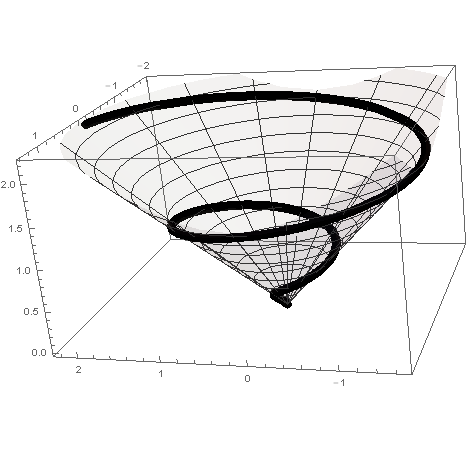
\includegraphics[scale=0.35]{gr-fig-9a.png}
	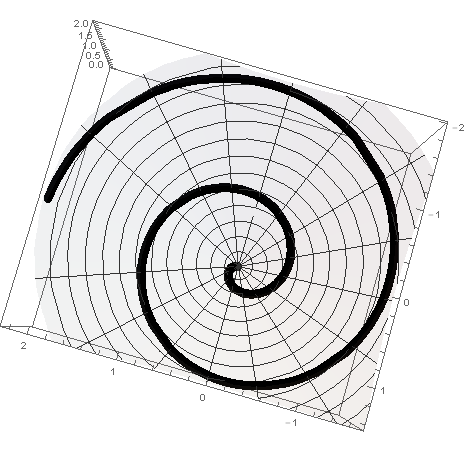
\includegraphics[scale=0.35]{gr-fig-9b.png}
	\caption{The underlying curve of path $\vec{r}(t)$, for $0 \leq t \leq \pi$, side view and top view.}
\end{figure}
Find the length of a curve is only ``mechanical'' once we already know the line element $ds^2$, which we have derived in the previous example. Plus, we know that $d\theta = 0$ since $\theta$ is constant. So,
\begin{align*}
L &= \int\,ds\\ 
&= \int_{0}^{\pi}\sqrt{\frac{dr^2}{dt^2} + r^2\frac{d\theta^2}{dt^2} + r^2\sin^2\theta\frac{d\phi^2}{dt^2}}\,dt\\
&= \int_{0}^{\pi}\sqrt{1 + 0 + \left( 4t\sin\left(\frac{\pi}{4} \right) \right) ^2}\,dt\\
&= \int_{0}^{\pi}\sqrt{1 + 8t^2}\,dt\\
&\approx 14.55. 
\end{align*}
\end{exmp}
As we have seen before in the earlier sections, the metric tensor does not just encode physical lengths. $g_{ij}$ are also ubiquitous in calculating norms of vectors and inner products (or dot products). As a reminder:
\begin{align*}
&\text{\textbf{Norm:} } \vert\vert \vec{\lambda} \vert\vert^2 = \vec{\lambda}\cdot\vec{\lambda} = g_{ij}\lambda^i\lambda^j\\
&\text{\textbf{Inner product:} } \vec{\lambda}\cdot\vec{\mu} = g_{ij}\lambda^i\mu^j.
\end{align*}
They can also be used to raise/lower indices, as we have seen. 
\subsubsection{Summations as matrix products}
As a little ``aside,'' writing vectors and 2-component tensors (such as $g_{ij}$) as matrices can be more convenient for us. But note that more general tensors (with three or more indices) can no longer be written as matrices.\\

Suppose that we have two square matrices $\tilde{A} = [a_{ij}]$ and $\tilde{B} = [b_{ij}]$. Let matrix $\tilde{C} = \tilde{A}\tilde{B}$. In matrix multiplication,
\begin{align*}
\boxed{
\tilde{C} = 
\begin{pmatrix}
&\vdots&\\
\dots&c_{ij}&\dots\\
&\vdots&
\end{pmatrix}
=
\begin{pmatrix}
\vdots&&\vdots\\
a_{i1} & \dots & a_{in}\\
\vdots&&\vdots
\end{pmatrix}
\begin{pmatrix}
\dots&b_{1j}&\dots\\
&\vdots&\\
\dots&b_{nj}&\dots
\end{pmatrix}
}
\end{align*} 
i.e., the $ij^{th}$ element of $\tilde{C}$ is 
\begin{align*}
\boxed{c_{ij} = \sum_{k=1}^na_{ik}b_{kj}}
\end{align*}
where $k$ on the $a$ term indicates a column, while $k$ on the $b$ term indicates a row. Notice that the summed index ($k$) goes as ``column-row,'' whereas $i-j$ go as row-column. Note that I do not have a restriction on $n$, because the above relations are true in any $n$-dimensional space. \\

Similarly, we can multiply vectors in matrix notations. Let two vectors $\vec{F}, \vec{G} \in \mathbb{R}^n$ be given. Assuming that the metric is the identity, their inner product is given by:
\begin{align*}
\boxed{
\vec{F}\cdot\vec{G} = 
\begin{pmatrix}
f_1\\
\vdots\\
f_n
\end{pmatrix}\cdot
\begin{pmatrix}
g_1\\
\vdots\\
g_n
\end{pmatrix}
=
\vec{F}^\top\vec{G} 
=
\sum_{k=1}^{n}f_kg_k.
}
\end{align*}
With a general metric $g_{ij}$, we want to express $\vec{\lambda}\cdot\vec{\mu} = g_{ij}\lambda^i\mu^j$ as a matrix multiplication. We have to make sure that the matrix multiplication is defined, i.e., the rows of the right-multiplying element is equal to the columns of the left-multiplying element. There are two things we can do: ordering the $ij$ indices, and transposing. Let $\tilde{\lambda}$ denote $\vec{\lambda} = [\lambda^i]$, and $\tilde{\mu}$ denote $\vec{\mu} = [\mu^i]$.
\paragraph{For contravariant vectors:\\}
Let $\tilde{G} = [g_{ij}]$, where $i$ is the row indicator and $j$ is the column indicator. This means that the index of $\vec{\lambda}$ has to be a column indicator, so we transpose $\vec{\lambda}$. The index of $\mu$ is a row indicator, which matches with $j$-the column indicator of $\tilde{G}$, so we are good to proceed. Again, note that $n$ is not necessarily 3.  
\begin{align*}
\boxed{
\vec{\lambda}\cdot\vec{\mu} = 
\lambda^ig_{ij}\mu^j
=
\begin{pmatrix}
\lambda_1 & \dots & \lambda_n
\end{pmatrix}
\begin{pmatrix}
g_{11} & \dots & g_{1n}\\
\vdots & \ddots & \vdots \\
g_{n1} & \dots & g_{nn}
\end{pmatrix}
\begin{pmatrix}
\mu_1 \\
\vdots\\
\mu_n
\end{pmatrix}
=
\tilde{\lambda}^\top \tilde{G} \tilde{\mu}}
\end{align*}
\paragraph{For covariant vectors:\\}
We can find express the inner product of covariant vectors in matrix multiplication, using the form we have found for contravariant products. Consider two covariant vectors $\tilde{\lambda}^* = [\lambda_i]$ and $\tilde{\mu}^* = [\mu_i]$ and the inverse metric tensor $\tilde{G}^{-1} = [g_{ij}]^{-1} = [g^{ij}]$ (recall that $g_{ij}g^{jk} = \delta^k_i$). Similar to the contravariant vector case, but now with $\vec{\lambda}\cdot\vec{\mu} = g^{ij}\lambda_i\mu_j$:
\begin{align*}
\boxed{
\tilde{\lambda}^*\cdot\tilde{\mu}^* = 
\begin{pmatrix}
\lambda_1 & \dots & \lambda_n
\end{pmatrix}
=
\begin{pmatrix}
g^{11} & \dots & g^{1n}\\
\vdots & \ddots & \vdots \\
g^{n1} & \dots & g^{nn}
\end{pmatrix}
\begin{pmatrix}
\mu_1 \\
\vdots\\
\mu_n
\end{pmatrix}
=
\tilde{\lambda}^{*\top}\tilde{G}^{-1}\tilde{\mu}
}
\end{align*}
As an little aside, to write $\tilde{\lambda}^*$ in terms of the metric tensor matrix and the contravariant vector, we simply remember that $\lambda_i = g_{ij}\lambda^j$. So,
\begin{align*}
&\tilde{\lambda}^* = \tilde{G}\tilde{\lambda}\\
&\tilde{\lambda} = \tilde{G}^{-1}\tilde{\lambda}^*
\end{align*}
In matrix form, the above two equalities can be written as:
\begin{align*}
\begin{pmatrix}
\lambda_1 \\
\vdots\\
\lambda_n
\end{pmatrix}
&=
\begin{pmatrix}
g_{11} & \dots & g_{1n}\\
\vdots & \ddots & \vdots\\
g_{n1} & \dots & g_{nn}
\end{pmatrix}
\begin{pmatrix}
\lambda^1\\
\vdots\\
\lambda_n
\end{pmatrix}
\end{align*}
and
\begin{align*}
\begin{pmatrix}
\lambda^1 \\
\vdots\\
\lambda^n
\end{pmatrix}
&=
\begin{pmatrix}
g^{11} & \dots & g^{1n}\\
\vdots & \ddots & \vdots\\
g^{n1} & \dots & g^{nn}
\end{pmatrix}
\begin{pmatrix}
\lambda_1\\
\vdots\\
\lambda_n
\end{pmatrix}
\end{align*}
respectively.\\
\paragraph{Metric tensor and inverse metric tensor\\}
As mentioned, $[g^{ij}] = [g_{ij}]^{-1}$. In matrix form:
\begin{align*}
\boxed{
\tilde{G}^{-1}\tilde{G} = 
\begin{pmatrix}
g^{11} & \dots & g^{1n}\\
\vdots & \ddots & \vdots \\
g^{n1} & \dots & g^{nn}
\end{pmatrix}
\begin{pmatrix}
g_{11} & \dots & g_{1n}\\
\vdots & \ddots & \vdots\\
g_{n1} & \dots & g_{nn}
\end{pmatrix}
=
\text{diag}(1,\dots,1) 
=
\tilde{I}
}
\end{align*}
\begin{exmp}
Find the inverse metric tensor $g^{ij}$ in spherical coordinates, given the metric tensor $g_{ij}$ is:
\begin{align*}
[g_{ij}] = 
\begin{pmatrix}
1 & 0 & 0\\
0 & r^2 & 0\\ 
0 & 0 & r^2\sin^2\theta 
\end{pmatrix}
\end{align*}
By definition, $[g^{ij}] = [g_{ij}]^{-1}$. So taking the inverse of $[g_{ij}]$ will give us $[g^{ij}]$. But notice that $[g_{ij}]$ is diagonal, so $g^{ij}$ is simply the reciprocal of $g_{ij}$, if $g_{ij} \neq 0$, and $0$ otherwise. This gives
\begin{align*}
[g^{ij}] = 
\begin{pmatrix}
1 & 0 & 0 \\
0 & r^{-2} & 0\\
0 & 0 & r^{-2}\sin^{-2}\theta
\end{pmatrix}
\end{align*}
\end{exmp}
\subsection{Coordinate transformation}
We have already seen the usage of multiple (more or less conventional) coordinate systems in the three-dimensional space. In general $n$-dimensional spaces, the options for coordinate systems are almost unlimited. It is crucial for us, as relativists, to develop for rigorous procedure to transform vector and tensor components as we move from one coordinate system to another. Note that vector and tensor \textbf{components} change under general coordinate transformation. It is common in physics to associate a vector or a tensor with a physical quantity, and coordinate system, or reference frame, etc., with perspectives. It makes sense that what we see might differ at different perspectives, but the physical quantity itself is independent of how we view it. In other words, vectors and tensors do not change under general coordinate transformations, only their components do.\\

In this subsection, we will learn how to transform between arbitrary coordinate systems. We will also learn how vector and tensor components transform, as well as what vectors and tensors are.
\subsubsection{Vectors}
We as physicists often think of vectors as an object with magnitude and direction. But this definition is incomplete, as it disregards a reference frame in which the vector is viewed. As we have mentioned in the introduction to this section, under general coordinate transformations, vectors do not change, but their components do, since the basis set of the coordinate system changes. For instance,
\begin{align*}
\text{insert figure 10 here!!!}
\end{align*}
\begin{align*}
\text{insert figure 11 here!!!}
\end{align*}
In the above two figures, the vector $\vec{\lambda}$ is the same. However, one frame is rotated by $\theta$ from another. In frames $(S)$ and $(S')$, $\vec{\lambda}$ will have different components, but the ``physical object'' $\vec{\lambda}$ does not change. For instance, we can calculate the norm of $\vec{\lambda}$, $\vert\vert \vec{\lambda} \vert\vert$, and find that it is the same in both frames. In fact, \textbf{scalars are invariant under general coordinate transformations}.\\

Next, let's talk \textbf{notations}. Let's assume, without loss of generality, that we are only dealing with contravariant vectors here (the rules we will establish shortly will apply to covariant vectors as well). Consider $\vec{\lambda}$ in frame $(S)$. In index-notation, we can write $\vec{\lambda} = \{\lambda^i\}$. Consider a different frame (a ``primed'' frame), denoted $(S')$. We will denote the components of $\vec{\lambda}$ in $(S')$ as $\lambda^{i'}$. Just to get us familiar with the new notation, let's go through an example:
\begin{exmp}
Suppose that $\vec{\lambda}$ is described two coordinate systems: spherical and cylindrical. Let the ``unprimed'' coordinate system be the spherical coordinate system. Then,
\begin{align*}
\{u^i\} &= (r,\theta,\phi)\\
\{u^{i'}\} &= (\rho, \phi, z).
\end{align*}
As simple as that!
\end{exmp}

Back to $(S)$ and $(S')$. Since these are two different coordinate systems, the basis sets and metric tensors are also different:
\begin{align*}
(S): &\text{ }\vec{e}_i = \frac{\partial \vec{r}}{\partial u^i}, \text{ }\vec{e}^{\,i} = \vec{\nabla}u^i, \text{ }g_{ij} = \vec{e}_i\cdot\vec{e}_j\\
(S'): &\text{ }\vec{e}_{i'} = \frac{\partial \vec{r}}{u^{i'}}, \text{ }\vec{e}^{\,i'} = \vec{\nabla} u^{i'}, \text{ }g_{i'j'} = \vec{e}_{i'}\cdot\vec{e}_{j'}.
\end{align*}
Now, since $\vec{\lambda}$ is the same in both $(S)$ and $(S')$, it must be true that"
\begin{align*}
\vec{\lambda} = \lambda^i\vec{e}_i = \lambda^{i'}\vec{e}_{i'},
\end{align*}
i.e., $\lambda^i$ and $\vec{e}_i$ must transform in a way that leaves $\vec{\lambda}$ unchanged. Consider $\vec{r} = \vec{r}(u^{i'}) = \vec{r}(u^{i'}(u^j))$. By the chain rule:
\begin{align*}
\vec{e}_j = \frac{\partial \vec{r}}{\partial u^j} = \frac{\partial \vec{r}}{\partial u^{i'}}\frac{\partial u^{i'}}{\partial u^j} = \vec{e}^{\,i'}\frac{\partial u^{i'}}{\partial u^j}.
\end{align*}
Let us define, for simplicity sake,
\begin{align*}
\boxed{U^{i'}_j = \frac{\partial u^{i'}}{\partial u^j}}
\end{align*}
Note that there is nothing new here. $U^{i'}_j$ simply generalizes 9 partial derivatives (because we are in 3-dimensional space). Together as a matrix, $[U^{i'}_j]$ is nothing but the Jacobian matrix ``representing'' the transformation $(S) \rightarrow (S')$:
\begin{align*}
[U^{i'}_j] = 
\begin{pmatrix}
\frac{\partial u^{1'}}{\partial u^1} & \frac{\partial u^{1'}}{\partial u^2} & \frac{\partial u^{1'}}{\partial u^3}\\
\frac{\partial u^{2'}}{\partial u^1} & \frac{\partial u^{2'}}{\partial u^2} & \frac{\partial u^{2'}}{\partial u^3}\\
\frac{\partial u^{3'}}{\partial u^1} & \frac{\partial u^{3'}}{\partial u^2} & \frac{\partial u^{3'}}{\partial u^3}
\end{pmatrix}
\end{align*}
So, the chain rule for $\vec{e}_j$ becomes the general coordinate transformation rule for the natural basis sets $\vec{e}_{i'} \rightarrow \vec{e}_i$. 
\begin{align*}
\boxed{\vec{e}_j = U^{i'}_j\vec{e}_{i'}}
\end{align*}
Next, since $\vec{\lambda} = \lambda^{i'}\vec{e}_{i'} = \lambda^j\vec{e}_j = \lambda^jU^{i'}_j\vec{e}_{i'}$, we obtain the general coordinate transformation rule for contravariant vector components $\lambda^{i} \rightarrow \lambda^{i'}$: 
\begin{align*}
\boxed{\lambda^{i'} = U^{i'}_j\lambda^j}
\end{align*}
We can, of course, conjecture that the transformation rule for contravariant vector components $\lambda^{i'} \rightarrow \lambda^{i}$ is:
\begin{align*}
\boxed{\lambda^{i'} = U^{j}_{i'}\lambda^{i'}}
\end{align*}
and we would be correct. The ``proof'' follows here. First, we look at the Jacobian matrix representing the transformation $(S') \rightarrow (S)$:
\begin{align*}
[ U^{j}_{i'}]  = \left[ \frac{\partial u^j}{\partial u^{i'}}\right], 
\end{align*}
which is simply the inverse of $\left[ U^{i'}_j\right] $. So, it follows that:
\begin{align*}
[ U^{j'}_k] [ U^{k}_{i'}]  &= \text{diag}(1,\dots,1) = [\delta^{j'}_{i'}] = [ \delta^{j}_{i}] = \tilde{I},
\end{align*}
and 
\begin{align*}
[U^k_{i'}][U^{i'}_j] &= \text{diag}(1,\dots,1) = [\delta^k_{j}] = \tilde{I},
\end{align*}
because matrices that are inverses of each other are commutative. Element-wise:
\begin{align*}
\boxed{U^k_{i'} U^{i'}_j = \delta^k_j = \delta^{k'}_{j'}= U^{k'}_i U^i_{j'}}
\end{align*}
So we can now verify our little ``conjecture:''
\begin{align*}
\lambda^{i'} &= U^{i'}_j\lambda^j\\
U^k_{i'}\lambda^{i'} &= U^{i'}_jU^k_{i'}\lambda^j\\
U^k_{i'}\lambda^{i'} &= \delta^k_j\lambda^j\\
U^k_{i'}\lambda^{i'} &= \lambda^k.
\end{align*}
We notice that nothing makes $U^{i'}_j$ more special than $U^{i}_{j'}$. Also, while we use contravariant vectors more often than covariant vectors, nothing makes contravariant vectors more special than covariant vectors. So if transformation rules apply to contravariant vectors, we should also expect them to work for covariant vectors:
\begin{empheq}[box=\fbox]{align}
\lambda_{i'} &= U^{j}_{i'}\lambda_j \nonumber\\
\lambda_{i} &= U^{j'}_i\lambda_{j'} \nonumber
\end{empheq}
At this point it looks like we are inventing new mathematics by playing a little game of swapping indices, and it is reasonable for us to grow a little bit suspicious of what we are doing here. But we can show that our ``index-swapping intuition'' is correct. Let us consider (again) a vector $\vec{\lambda} = \lambda_j\vec{e}^{\,j} = \{ \lambda_j\}$, where $\vec{e}^{\,j}$ is a vector in the dual basis:
\begin{align*}
\vec{e}^{\,j} = \vec{\nabla}u^j = \frac{\partial u^j}{\partial x}\hat{i} + \frac{\partial u^j}{\partial y}\hat{j} + \frac{\partial u^j}{\partial z}\hat{k}.
\end{align*}
Let us apply to chain rule:
\begin{align*}
\frac{\partial u^j}{\partial x} = \frac{\partial u^j}{\partial u^{i'}}\frac{\partial u^{i'}}{\partial x}.
\end{align*}
Therefore,
\begin{align*}
\vec{e}^{\,j} &= \vec{\nabla}u^j\\
&= \frac{\partial u^j}{\partial x}\hat{i} + \frac{\partial u^j}{\partial y}\hat{j} + \frac{\partial u^j}{\partial z}\hat{k}\\
&= \frac{\partial u^j}{\partial u^{i'}}\frac{\partial u^{i'}}{\partial x}\hat{i} + \frac{\partial u^j}{\partial u^{i'}}\frac{\partial u^{i'}}{\partial y}\hat{j} + \frac{\partial u^j}{\partial u^{i'}}\frac{\partial u^{i'}}{\partial z}\hat{k}\\
&= \sum_{i=1}^{3}\frac{\partial u^j}{\partial u^{i'}}\frac{\partial u^{i'}}{\partial x}\hat{i} + \frac{\partial u^j}{\partial u^{i'}}\frac{\partial u^{i'}}{\partial y}\hat{j} + \frac{\partial u^j}{\partial u^{i'}}\frac{\partial u^{i'}}{\partial z}\hat{k}\\
&= \sum_{i=1}^{3}\frac{\partial u^j}{\partial u^{i'}}\left( \frac{\partial u^{i'}}{\partial x}\hat{i} + \frac{\partial u^{i'}}{\partial y}\hat{j} + \frac{\partial u^{i'}}{\partial z}\hat{k}\right) \\
&= \sum_{i=1}^{3}\frac{\partial u^j}{\partial u^{i'}}\vec{\nabla}u^{i'}\\
&= \sum_{i=1}^{3}U^{j}_{i'}\vec{e}^{\,i'}.
\end{align*}
Or, in Einstein's summation notation, the transformation rule for the dual basis vectors is:
\begin{align*}
\boxed{\vec{e}^{\,j} = U^j_{i'}\vec{e}^{\,i'}}
\end{align*}
And the inverse transformation follows:
\begin{align*}
\boxed{\vec{e}^{\,j'} = U^{j}_{i'}\vec{e}^{\,i'}}
\end{align*}
Note that, the above relation is in fact true for any $n$-dimensional space. Our ``proof'' here is restricted to only 3-dimensional space. However, it is not so difficult to fix this slight issue. If we redefine the $\vec{\nabla}$ operator for $n$-dimensional space, then we can easily see that the new proof is identical to the proof above, except for the maximal value of $n$. \\

We easily obtain the transformation rules for the covariant vector components using the results above:
\begin{align*}
\vec{\lambda} = \lambda_{i'}\vec{e}^{\,i'} = \lambda_j\vec{e}^{\,j} = \lambda_jU^j_{i'}\vec{e}^{\,i'} = \lambda_{i'}U^{i'}_j\vec{e}^{\,j}.
\end{align*}
Therefore,
\begin{empheq}[box=\fbox]{align}
\lambda_{i'} &= U^j_{i'}\lambda_j \nonumber\\
\lambda_j &= U^{i'}_j\lambda_{i'} \nonumber
\end{empheq}
Below is a summary of what we have learned so far about general coordinate transformations:
\[
\boxed{
\begin{matrix}
\text{\textbf{Natural basis:} }& \vec{e}_j = U^{i'}_j\vec{e}_{i'} & \vec{e}_{j'} = U^{i}_{j'}\vec{e}_{i} \\
\text{\textbf{Dual basis:} }& \vec{e}^{\,j} = U^{j}_{i'}\vec{e}^{\,i'} & \vec{e}^{\,j'} = U^{j'}_i\vec{e}^{\,i}\\
\text{\textbf{Contravariants:} } & \vec{\lambda}^{j'} = U^{j'}_i\vec{\lambda}^{i} & \vec{\lambda}^j = U^{j}_{i'}\vec{\lambda}^{i'}\\
\text{\textbf{Covariants:} } & \vec{\lambda}_j = U^{i'}_j\vec{\lambda}_{i'} & \vec{\lambda}_{j'} = U^{i}_{j'}\vec{\lambda}^{j'}\\
\end{matrix}
}
\]
Since components of a vector must transform according to the rules above under general coordinate transformations, we can turn these rules into a more general definition of a vector.
\begin{defn}
	A vector is a quantity whose components transform contravariantly as $\lambda^{i'} = U^{i'}_j\lambda^j$ under a general coordinate transformation $u^{i'} = u^{i'}(u^j)$.
\end{defn}
\begin{rmk}
	We are often interested in vector fields, a collection of vectors at different points in space whose components depend on the coordinates: $\lambda^i = \lambda^i(u^j)$. Since vectors have to transform correctly, we require that at any point $P$, we require that $\lambda^{i'} = U^{i'}_j\lambda^j$ be true for a vector field (defined on $\lambda^i$) to be defined. 
\end{rmk}
\begin{rmk}
	Not all 3-tuple of functions are vectors. Consider a 3-tuple of coordinates. Let $\lambda^i = u^i$ and $\lambda^{j'} = u^{j'}$, where $u^{j'} = u^{j'}(u^i)$. For $\lambda^i$ to be make a vector field, it is required that $\lambda^{i'} = U^{i'}_j\lambda^j$. This implies that $u^{i'} = U^{i'}_ju^j$, with $U^{i'}_j = \partial u^{i'}/\partial u^j$. However, we immediately see that this is \textbf{not true in general}:
	\begin{align*}
	\boxed{u^{i'} \neq \frac{\partial u^{i'}}{\partial u^j}u^j}
	\end{align*}
	But rather, $u^{i'} = u^{i'}(u^j) = f(u^j)$. So, coordinates themselves do not make vectors in general, because they, as components, do not transform correctly under general coordinate transformations. This is why we never use $g_{ij}$ or $g^{ij}$ to lower or raise the index of $u^i$ or $u_i$, i.e., $u^i \neq g^{ij}u_j$, and $u_j \neq g_{ij}u^i$, in general. \\
	
	There are exemptions to the ``general rule,'' of course. For instance, consider \textbf{linear transformations}, where $u^{j'} = u^{j'}(u^i) = C^{j'}_iu^i$, where $C^{j'}_i$ are constants. What this means is that the new coordinates are simply linear combinations of the old coordinates. It follows that
	\begin{align*}
	\frac{\partial u^{j'}}{\partial u^k} = C^{j'}_i\frac{\partial u^i}{\partial u^k} = C^{j'}_i\delta^i_k=C^{j'}_k.
	\end{align*}
	If we let $k=i$ (we're just swapping dummy indices here), then $C^{j'}_i = \partial u^{j'}/\partial u^i = U^{j'}_i$, i.e., $u^{j'} = U^{j'}_iu^i$ under linear transformations. Therefore, $u^i$ transform correctly, and in this case the coordinates $u^i$ can form a vector, $\{u^i\}$.
\end{rmk}
\begin{rmk}
	Properly speaking we can define vectors with respect to a particular class of transformations. It is possible for something to be a vector with respect to a class of transformation, but not a vector with respect to another. Such a class of transformation (default) is the general coordinate transformations. 
\end{rmk}
\begin{exmp}
	Can differentials of coordinates ($du^i$) form a vector?\\
	
	The solution is actually quite simple. Without loss of generality, let us consider a hypothetical vector $\{ du^i \}$ in 3-dimensional space. $\{du^1, du^2, du^3 \}$. Applying the chain rule:
	\begin{align*}
	du^{i'} = \frac{\partial u^{i'}}{\partial u^{j}}\,du^j = U^{i'}_j\,du^j.
	\end{align*}
	We see that $du^i$ transform correctly under general coordinate transformations. Therefore, $du^i$ can make a vector. 
\end{exmp}
\begin{exmp}
	Find $[U^{j'}_i]$ for a coordinate transformation from Cartesian to spherical in flat 3-dimensional space. Let $\{u^j\} = \{ x,y,z\}$ and $\{u^{j'} \} = \{ r, \theta, \phi\} $. We find the Jacobian matrix:
	\begin{align*}
	[U^{j'}_i] = 
	\begin{pmatrix}
	\frac{\partial r}{\partial x} & \frac{\partial r}{\partial y} & \frac{\partial r}{\partial z}\\
	\frac{\partial \theta}{\partial x} & \frac{\partial \theta}{\partial y} & \frac{\partial \theta}{\partial z}\\
	\frac{\partial \phi}{\partial x} & \frac{\partial \phi}{\partial y} & \frac{\partial \phi}{\partial z}
	\end{pmatrix}
	=\frac{1}{r}
	\begin{pmatrix}
	r\sin\theta\cos\phi & r\sin\theta\sin\phi & r\cos\theta\\
	\cos\theta\cos\phi & \cos\theta\sin\phi & -\sin\theta\\
	\frac{-\sin\phi}{\sin\theta} & \frac{\cos\phi}{\sin\theta} & 0
	\end{pmatrix}
	\end{align*}
\end{exmp}
\begin{exmp}
	Consider $\vec{\lambda} = (1,0,0)^\top = \{\lambda^{i'}\}$ in Cartesian coordinates. What are the components of $\vec{\lambda}$ in spherical coordinates? \\
	
	With our developed procedure, we should be able to obtain the answer with little thinking:
	\begin{align*}
	\vec{\lambda} = \{ \lambda^{i'} \} = 
	\begin{pmatrix}
	\lambda^{1'} \\ \lambda^{2'} \\ \lambda^{3'}
	\end{pmatrix}
	=
	[U^{i'}_j\lambda^j]
	= 
	\frac{1}{r}
	\begin{pmatrix}
	r\sin\theta\cos\phi & r\sin\theta\sin\phi & r\cos\theta\\
	\cos\theta\cos\phi & \cos\theta\sin\phi & -\sin\theta\\
	\frac{-\sin\phi}{\sin\theta} & \frac{\cos\phi}{\sin\theta} & 0
	\end{pmatrix}
	\begin{pmatrix}
	1 \\ 0 \\ 0
	\end{pmatrix},
	\end{align*}
	which gives
	\begin{align*}
	\begin{pmatrix}
	\lambda^{1'} \\ \lambda^{2'} \\ \lambda^{3'}
	\end{pmatrix}
	=
	\frac{1}{r}
	\begin{pmatrix}
	r\sin\theta\cos\phi\\
	\cos\theta\cos\phi\\
	\frac{-\sin\phi}{\sin\theta}
	\end{pmatrix}.
	\end{align*}
	In the natural basis of spherical coordinates, 
	\begin{align*}
	\vec{\lambda} = \sin\theta\cos\phi\,\vec{e}_r + \frac{1}{r}\cos\theta\cos\phi\,\vec{e}_\theta - \frac{\sin\phi}{r\sin\theta}\,\vec{e}_\phi.
	\end{align*}
	We have said before that the ``physical quantity'' $\vec{\lambda}$ does not change. We can test this by finding $\vert\vert \vec{\lambda} \vert\vert$ in Cartesian and spherical coordinates and compare the results. In Cartesian, the metric tensor is $g_{ij} = \delta^j_i$, so
	\begin{align*}
	\vert\vert \vec{\lambda} \vert\vert_{\text{Cartesian}} = \sqrt{g_{ij}\lambda^i\lambda^j} = \sqrt{1^2 + 0^2 + 0^2} = 1,
	\end{align*}
	as expected. The metric tensor $g_{i'j'}$ of spherical coordinate, in matrix form, is:
	\begin{align*}
	[g_{i'j'}] = \begin{pmatrix}
	1 & 0 & 0\\
	0 & r^2 & 0\\
	0 & 0 & r^2\sin^2\theta
	\end{pmatrix}.
	\end{align*}
	It follows that
	\begin{align*}
	\vert\vert \vec{\lambda} \vert\vert_{\text{Spherical}} &= \sqrt{g_{i'j'}\lambda^{i'}\lambda^{j'}} = g_{1'1'}\left( \lambda^{1'}\right) ^2 + g_{2'2'}\left( \lambda^{2'}\right) ^2 + g_{3'3'}\left( \lambda^{3'}\right) ^2\\
	&= \sqrt{\left( \sin\theta\cos\phi\right)^2 + r^2\left(\frac{1}{r}\cos\theta\cos\phi \right)^2 + r^2\sin^2\theta\left(-\frac{\sin\phi}{r\sin\theta} \right)^2  }\\
	&= \sqrt{\left( \sin\theta\cos\phi\right)^2 + \left(\cos\theta\cos\phi \right)^2 + \sin^2\phi}\\
	&= \sqrt{\cos^2\phi + \sin^2\phi}\\
	&= 1.
	\end{align*}
	Not surprisingly, $\vert\vert \vec{\lambda}_{\,\text{Cartesian}} \vert\vert = \vert\vert \vec{\lambda}_{\,\text{Spherical}} \vert\vert = 1$.
\end{exmp}
\begin{exmp}
	Find $U^{j'}_i$ for a rotation by an angle $\phi$ around the $z$-axis in Cartesian coordinates. Suppose $\vec{a} = \{a^i \}= (1,1,0)^\top$. What is $\vec{a} = \{ a^{i'}\}$ after a rotation by $\phi$?
	\begin{align*}
	\text{insert figure 12 here!!!}
	\end{align*}
	From linear algebra, we know that a rotation by $\phi$ around the $z$-axis is given by:
	\begin{align*}
	\begin{pmatrix}
	x'\\y'\\z'
	\end{pmatrix}
	=
	\begin{pmatrix}
	\cos\phi & -\sin\phi & 0\\
	\sin\phi & \cos\phi & 0 \\
	0 & 0 & 1
	\end{pmatrix}
	\begin{pmatrix}
	x\\y\\z
	\end{pmatrix}.
	\end{align*}
	So,
	\begin{align*}
	[U^{j'}_i] = 
	\begin{pmatrix}
	\cos\phi & -\sin\phi & 0\\
	\sin\phi & \cos\phi & 0 \\
	0 & 0 & 1
	\end{pmatrix}
	\end{align*}
	Given that $\vec{a} = \{a^i \}= (1,1,0)^\top$, 
	\begin{align*}
	\begin{pmatrix}
	\lambda^{1'}\\\lambda^{2'}\\\lambda^{3'}
	\end{pmatrix}
	=
	\begin{pmatrix}
	\cos\phi & -\sin\phi & 0\\
	\sin\phi & \cos\phi & 0 \\
	0 & 0 & 1
	\end{pmatrix}
	\begin{pmatrix}
	1\\1\\0
	\end{pmatrix}
	=
	\begin{pmatrix}
		\cos\phi - \sin\phi\\
		\sin\phi + \cos\phi\\
		0
	\end{pmatrix}
	\end{align*}
	Notice that because the coefficients of $[U^{j'}_i]$ are constants, the coordinates $\{ x,y,z\}$ can make a vector. But note (again) that this is not true in general.\\
	
	Next, we can find $\vert\vert \vec{\lambda} \vert\vert$ in both coordinate systems again and show that they are equal. In Cartesian coordinates, $\{\lambda^i\} = (1,1,0)^\top$. So, $\vert\vert \vec{\lambda} \vert\vert = \sqrt{2}$. In the rotated frame:
	\begin{align*}
	\vert\vert\vec{\lambda}\vert\vert = \sqrt{g_{i'j'}\lambda^{i'}\lambda^{j'}}.
	\end{align*}
	We seem to be stuck here, since we have yet found the form of the new metric $g_{i'j'}$. However, we observe that $g_{i'j'} = e^{i'}\cdot\vec{e}_{j'}$, which is just either 1 (if $i=j$) or 0 (if $j\neq j$), because the new coordinate system is just the ``tilted'' version of the old one. So we expect that new metric tensor is the same as the old metric tensor, which is nothing but $g_{i'j'}=\text{diag}(1,1,1)$. We can proceed to calculate the norm:
	\begin{align*}
	\vert\vert\vec{\lambda}\vert\vert &= \sqrt{\left( \cos\phi - \sin\phi \right)^2 + \left( \sin\phi + \cos\phi \right)^2 + 0^2}\\
	&= \sqrt{2\left(\sin^2\phi + \cos^2\phi\right) }\\
	&= \sqrt{2},
	\end{align*}
	which is of course what we found earlier. 
\end{exmp}
The above example motivates what we will discuss next. We have seen how vector components transform under general coordinate transformations, and how their norms (scalar) remain invariant. However, we start to question how the metric tensor transforms, in general. In the above example, the only reason we was able to calculate the norm of $\vec{\lambda}$ was that we could guess the form of the metric tensor, using some cleverness. In general, though, we will not be able to solve this problem without knowing exactly the form of the metric. Our next task, as apparent as it is now, is to find out how metric tensors in particular and tensors in general transform under general coordinate transformations. 
\subsubsection{Tensors}
We should first ask ourselves what tensors are. While a rigorous definition of a tensor will come shortly in this section (hint: it will resemble that of a vector, i.e., based on how their components transform under general coordinate transformations), we can first think of tensors as generalizations of vectors, i.e., with more than one index and hence multi-dimensional. Consider a physical object like a balloon which stretches and compresses multi-dimensionally when some force is applied to it. We call this ``response'' the stress tensor, which has 9 components in 3-dimensional space: $F_{xx}, F_{xy}, F_{xz}, F_{yx}, F_{yy}, F_{yz}, F_{zx}, F_{zy}, F_{zz}$.  
\begin{defn}
	A tensor is a multi-component quantity whose components transform as contravariant or covariant vector components.
\end{defn}
\begin{exmp}
	Find the condition for $\tensor{\tau}{^{ij}_k^l}$ to be a tensor.\\
	
	Well, a tensor has to transform correctly, so we can play a little game of index-replacing:
	\begin{align*}
	\boxed{\tensor{\tau}{^{i'j'}_{k'}^{l'}} = U^{i'}_mU^{j'}_nU^p_{k'}U^{l'}_p\tensor{\tau}{^{mn}_{p}^{q}}}
	\end{align*}
	under a general coordinate transformation $u^{i'} \rightarrow u^{i'}(u^j)$. 
\end{exmp}
\begin{exmp}
	Show that $g_{ij}$ is a tensor.\\
	
	$g_{ij}$ is a tensor, in fact, by definition:
	\begin{align*}
	\boxed{g_{i'j'} = U^k_{i'}\vec{e}_k \cdot U^l_{j'}\vec{e}_l = U^k_{i'}U^l_{j'}\vec{e}_k \cdot\vec{e}_l = U^k_{i'}U^l_{j'}g_{kl}}
	\end{align*} 
	Similarly, the inverse $g^{ij}$ is also a tensor:
	\begin{align*}
	\boxed{g^{k'l'} = U^{k'}_{i}\vec{e}^{\,i} \cdot U^{l'}_{j}\vec{e}^{\,j} = U^{k'}_iU^{l'}_{j}\vec{e}^{\,i} \cdot\vec{e}^{\,j} = U^{k'}_{i}U^{l'}_{j}g^{ij}}
	\end{align*}
\end{exmp}
\begin{defn}
	A tensor $\tensor{\tau}{^{abc\dots}_{def\dots}}$ is of type $(r,s)$ when it has $r$ contravariant components and $s$ covariant components. 
\end{defn}
\begin{exmp}
	$g_{ij}$ is a type $(0,2)$ tensor. $g^{ij}$ is a type $(2,0)$ tensor. 
\end{exmp}
Vectors are just a special type of tensors. Contravariant vectors $\lambda^i$ are type $(1,0)$ tensors, while covariant vectors $\lambda_i$ are type $(0,1)$ tensors. 
\begin{rmk}
	The transformation $U^{i'}_j$ is NOT a tensor. Indeed, it does not make sense to talk about how a transformation transforms. 
\end{rmk}
\begin{exmp}
	Write $g_{i'j'} = U^k_{i'}U^l_{j'}g_{kl}$ as a matrix equation.\\
	
	We let $\tilde{G} = [g_{ij}]$, $\tilde{G}'= [g_{i'j'}]$, and $\hat{U} = \tilde{U}^{-1} = [\partial u^k/\partial u^{i'}]$. To create a matrix equation, we have to be aware of when an index indicate a row or column. The correct ``row-column-sensitive'' order expression is:
	\begin{align*}
	[g_{i'j'}] &= [U^{k}_{i'}][g_{kl}][U^l_{j'}],
	\end{align*}
	or equivalently,
	\begin{align*}
	\boxed{\tilde{G}' = \hat{U}^{\top}\tilde{G}\hat{U}}
	\end{align*}
\end{exmp}
\begin{exmp}
	Using the transformation rules for tensors, obtain $g_{i'j'}$ for a rotation by $\phi$ around the $z$-axis in 3-dimensional space. \\
	
	Recall that
	\begin{align*}
	[U^{j'}_i] = 
	\begin{pmatrix}
	\cos\phi & -\sin\phi & 0\\
	\sin\phi & \cos\phi & 0 \\
	0 & 0 & 1
	\end{pmatrix},
	\end{align*}
	and that $g_{ij} = \text{diag}(1,1,1)$ in 3-dimensional Cartesian coordinate system. To find $\tilde{G}'$, we first have to find $U^k_{i'}$, the inverse transformation. We expect that $U^k_{i'}$ is simply a rotating by $-\phi$ (since this intuitively ``reverses'' what $U^{k'}_{i}$ does). But we, as always, find $U^k_{i'}$ mechanically:
	\begin{align*}
	\hat{U} = \left[\frac{\partial u^k}{\partial u^{i'}} \right]  =\tilde{U}^{-1} = 
	\begin{pmatrix}
	\cos\phi & -\sin\phi & 0\\
	\sin\phi & \cos\phi & 0 \\
	0 & 0 & 1
	\end{pmatrix}^{-1}
	=
	\begin{pmatrix}
	\cos\phi & \sin\phi & 0\\
	-\sin\phi & \cos\phi & 0 \\
	0 & 0 & 1
	\end{pmatrix},
	\end{align*} 
	as anticipated. Using the result of the previous example,
	\begin{align*}
	\tilde{G}' &= \hat{U}^{\top}\tilde{G}\hat{U}\\
	&= \begin{pmatrix}
	\cos\phi & \sin\phi & 0\\
	-\sin\phi & \cos\phi & 0 \\
	0 & 0 & 1
	\end{pmatrix}
	\begin{pmatrix}
	1 & 0 & 0\\
	0 & 1 & 0\\
	0 & 0 & 1
	\end{pmatrix}
	\begin{pmatrix}
	\cos\phi & -\sin\phi & 0\\
	\sin\phi & \cos\phi & 0 \\
	0 & 0 & 1
	\end{pmatrix}\\
	&=
	\begin{pmatrix}
	1 & 0 & 0\\
	0 & 1 & 0\\
	0 & 0 & 1
	\end{pmatrix},
	\end{align*}
	just as guessed. So our intuition was correct after all. But we realize an important fact: the metric tensor can remain the same after a non-trivial transformation (in this case the transformation is a rotating around the $z$-axis). We also notice that the metric tensors are the same under a transformation if the transformation matrix is \textbf{orthogonal}, i.e., its inverse the equal to its transpose:
	\begin{align*}
	\hat{U} = \tilde{U}^{-1} = \tilde{U}^\top.
	\end{align*}
\end{exmp}

\begin{rmk}
	Only tensors of type $(r,s)$ with $r+s \leq 2$ can be displayed as matrices and/or matrix multiplications. It is not possible to write $\tensor{\tau}{^{ij}_{kl}}$ as a matrix. 
\end{rmk}

\subsection{Scalars}
As we have seen from time to time, scalars are invariant under general coordinate transformations. As tensors, scalars are of type $(0,0)$, i.e., they have open indices.
\begin{exmp}
	Show that the magnitude of a vector is a scalar.\\
	
	Consider $\vec{a} = {a^i} = {a^{i'}}$ in two different coordinate systems. The magnitude of $\vec{a} = \vert\vert \vec{a} \vert\vert$ is a scalar if:
	\begin{align*}
	\vec{a}\cdot\vec{a} = a^ia_i = a^{i'}a_{i'}.
	\end{align*} 
	This can be readily shown, since we already know the transformation rules for vector components:
	\begin{align*}
	a^{i'}a_{i'} &= \left( U^{i'}_j a^j \right) \left( U^{k}_{i'}a_k\right) \\
	&= U^{i'}_j a^j U^{k}_{i'} a_k a^j\\
	&= \delta^{k}_j a_k a^j\\
	&= a^k a_k\\
	&= a^i a_i.
	\end{align*}
	Therefore, $\vert\vert \vec{a} \vert\vert$ is a scalar.
\end{exmp}
\begin{exmp}
	Show that the line element $ds^2 = g_{ij}\,du^i\,du^j$ is a scalar. \\
	
	Similar to the previous example, we have to show that:
	\begin{align*}
	g_{i'j'}\,du^{i'}\,du^{j'} = g_{ij}\,du^i\,du^j.
	\end{align*}
	We simply apply the transformation rule to each factor and play a little game of index-arranging:
	\begin{align*}
	g_{i'j'}\,du^{i'}\,du^{j'} &= \left( U^k_{i'} U^l_{j'} g_{kl}\right) \left(U^{i'}_m \,du^m \right) \left(U^{j'}_n \,du^n\right) \\
	&= U^k_{i'} U^l_{j'} U^{i'}_m U^{j'}_n g_{kl}\,du^m\,du^n\\
	&= \delta^k_m\delta^l_n \,g_{kl}\,du^m\,du^n\\
	&= g_{kl}\,du^k\,du^l\\
	&= g_{ij}\,du^i\,du^j.
	\end{align*}
	Therefore, $ds^2 = g_{ij}\,du^i\,du^j$ is a scalar.
\end{exmp}

\newpage

\section{Flat spacetime}
Recall that in space, we require 3 coordinates. It makes sense that in order to describe spacetime, we need an extra coordinate to describe time, in which case, we will switch from Roman-character indices ($i,j,k,\dots = 1,2,3$) to Greek-character indices $(\mu, \nu, \sigma, \dots) = 0,1,2,3$. We also tend to (by an unwritten convention and of course not mandatory) write vectors as capital letters to distinguish 4-vectors from 3-vectors. For example, below are a number of ways we express a 4-vector:
\begin{align*}
X^\mu = \left\{ X^0, X^1, X^2, X^3\right\} = \left( X^0, \vec{X} \right)  = \left( X^0, X^i\right) .
\end{align*}   
Notice that the ``hat'' notation is reserved for 3-vectors. 
\subsection{Special Relativity}
Coordinate transformations in special relativity are Lorentz transformations under which the spacetime interval (in Cartesian coordinates)
\begin{align*}
ds^2 = c^2\,dt^2 + dx^2 +dy^2+dz^2 = \left(dx^0 \right)^2 + \left(dx^1 \right)^2 + \left(dx^2 \right)^2 + \left(dx^3 \right)^2,
\end{align*}
which gives ``physical distances'' in spacetime, is invariant. We also recall that
\begin{align*}
ds^2 = g_{ij}\,du^i\,du^j,
\end{align*}
we can ``read off'' the metric from the spacetime interval as $\text{diag} = (1,-1,-1,-1)$. This is referred to as the Minkowski metric (flat 4-dimensional spacetime in Cartesian coordinates), denoted as $\eta_{\mu\nu}$:
\begin{align*}
[\eta_{\mu\nu}] = 
\begin{pmatrix}
1 & 0 & 0 & 0\\
0 & -1 & 0 & 0\\
0 & 0 & -1 & 0\\
0 & 0 & 0 & -1
\end{pmatrix}
\end{align*}
Because any frame in special relativity can be connected to the original frame by a Lorentz transformation, i.e.,
\begin{align*}
ds^2 = {ds'}^2 = \left(dx^{0'} \right)^2 + \left(dx^{1'} \right)^2  + \left(dx^{2'} \right)^2 + \left(dx^{3'} \right)^2, 
\end{align*}
The Minkowski metric (in Cartesian coordinates) is the same for any reference frame:
\begin{align*}
[\eta_{\mu'\nu'}] = [\eta_{\mu\nu}] = 
\begin{pmatrix}
1 & 0 & 0 & 0\\
0 & -1 & 0 & 0\\
0 & 0 & -1 & 0\\
0 & 0 & 0 & -1
\end{pmatrix}.
\end{align*}
This says that:
\begin{align*}
\boxed{ds^2 = \eta_{\mu\nu}\,dX^\mu\,dX^\nu = \eta_{\mu'\nu'}\,dX^{\mu'}\,dX^{\nu'}}
\end{align*}
For general coordinate systems in three dimensions, the metric $g_{ij} \neq \text{diag}(1,1,1)$. In these cases, the Minkowski metric has the following form:
\begin{align*}
[\eta_{\mu\nu}] = 
\begin{pmatrix}
1 & 0\\
0 & -[g_{ij}]
\end{pmatrix}
=
\begin{pmatrix}
1 & 0 & 0 & 0\\
0 & & &\\
0 & & -[g_{ij}] &\\
0 & & &
\end{pmatrix}.
\end{align*} 
More generally, however, spacetime can be curved, and the metric tensor of the three-dimensional space can be non-Cartesian. In these cases, we simply replace $\eta_{\mu\nu}$ by $g_{\mu\nu}$. It follows that:
\begin{align*}
\boxed{ds^2 = g_{\mu\nu}\,du^\mu\,du^\nu}
\end{align*}
in general. The ``moral'' here is that $\eta_{\mu\nu}$ is reserved for flat Minkowski spacetime. \\

Same as before, the metric tensor encodes all ``physical properties'' of the Minkowski spacetime and allows us to transform contravariant components into covariant components and vice versa. For instance, consider a contravariant vector $\lambda^\mu = (\lambda^0, \lambda^1, \lambda^2, \lambda^3) = (\lambda^0, \vec{\lambda})$. The covariant vector is given by simply ``lowering'' the index of the contravariant vector using the Minkowski metric tensor:
\begin{align*}
\lambda_\mu = \eta_{\mu\nu}\lambda^\nu = (\lambda_0, \lambda_1, \lambda_2, \lambda_3).
\end{align*}
The inverse transformation has the same form:
\begin{align*}
\lambda^\mu = \eta^{\mu\nu}\lambda_\nu.
\end{align*}
Note that if we use the Minkowski metric tensor in Cartesian coordinates, then
\begin{align*}
\lambda_\mu = \eta_{\mu\nu}\lambda^\nu = (\lambda_0, \lambda_1, \lambda_2, \lambda_3) = (\lambda^0, -\lambda^1, -\lambda^2, -\lambda^3).
\end{align*}
We observe that
\begin{align*}
\lambda^0 &= \lambda_0\\
\lambda^i &= -\lambda_i.
\end{align*}
We also observe that the inverse Minkowski metric tensor is Minkowski metric tensor itself:
\begin{align*}
\boxed{
[\eta^{\mu\nu}] = [\eta_{\mu\nu}]^{-1} 
= 
\begin{pmatrix}
1 & 0 & 0 & 0\\
0 & -1 & 0 & 0\\
0 & 0 & -1 & 0\\
0 & 0 & 0 & -1
\end{pmatrix}^{-1}
=
\begin{pmatrix}
1 & 0 & 0 & 0\\
0 & -1 & 0 & 0\\
0 & 0 & -1 & 0\\
0 & 0 & 0 & -1
\end{pmatrix}}
\end{align*}
Inner products of vectors follow the same rule as before:
\begin{align*}
\boxed{
\mathbf{a}\cdot\mathbf{b} = a^\mu b_\mu = a_\mu b^\mu = \eta_{\mu\nu}a^\mu b^\nu = \eta^{\mu\nu}a_\mu b_\nu}
\end{align*}
On a more practical side of things, we have to be careful with the signs that go with the terms when we solve problems:
\begin{align*}
\mathbf{a}\cdot\mathbf{b} &= a^1b_1 + a^2b_2 + a^2b_2 + a^3b_3\\
&= a_1b_1 - a_2b_2 - a_2b_2 - a_3b_3\\
&= a^1b^1 - a^2b^2 - a^2b^2 - a^3b^3.
\end{align*}
At this point, we might wonder what the basis vectors $\vec{e}_\mu$ in the flat, 4-dimensional Minkowski spacetime in Cartesian coordinates are. We can, of course, find them, from the metric tensor $\eta_{\mu\nu}$. However, one thing for sure: they are not going to be the basis vectors $\hat{i}, \hat{j}, \hat{k}$. In fact, the basis vectors that make up $\eta_{\mu\nu}$ will likely contain imaginary parts, since $\vec{e}_i\cdot\vec{e}_j = -1$ for $i = j$. The point is: we don't really need the basis vectors once we already have the metric, because after all, almost all of our computations involve the metric tensor. 
\subsubsection{The Lorentz Transformations, revisited} 
Recall that Lorentz transformations are (not necessarily strictly linear) transformations from one \textbf{inertial frame} $(S)$ to another \textbf{inertial frame} $(S')$.\\

The most general Lorentz transformations, also referred to collectively as ``Poincar\'e transformations'' include:
\begin{itemize}
	\item Lorentz boost: inertial frames with relative velocity $v$.
	\item Translation: origins don't coincide at $t'=t=0$.
	\item Spatial rotation
	\item Spatial inversion: or parity transformations ($x' = -x$)
	\item Time reversal: $t'=-t$.
\end{itemize} 
We can also make further distinctions among the listed transformations:
\begin{itemize}
	\item Inhomogeneous Lorentz transformations: have non-trivial translation.
	\item Homogeneous Lorentz transformations: no translations.
	\item Improper Lorentz transformations: with time reversal or parity.
	\item Proper Lorentz transformation: no parity or time reversal.
\end{itemize}
We can first look at \textbf{homogeneous, proper Lorentz transformations with no rotations}, i.e., Lorentz boosts. These are probably the simplest of Lorentz transformations that we encountered in introductory special relativity. A classic example is the Lorentz boost along the $x$-axis:
\begin{align*}
\begin{pmatrix}
a^{0'}\\a^{1'}\\a^{2'}\\a^{3'}
\end{pmatrix}
=
\begin{pmatrix}
\gamma & -\beta\gamma & 0 & 0\\
-\beta\gamma & \gamma & 0 & 0\\
0 & 0 & 1 & 0\\
0 & 0 & 0 & 1
\end{pmatrix}
\begin{pmatrix}
a^{0}\\a^{1}\\a^{2}\\a^{3}
\end{pmatrix}
\end{align*}
where the transformation matrix element $U^{i'}_j$ in 3-dimensional space is now generalized to 4-dimensional spacetime:
\begin{align*}
\boxed{X^{\mu'}_\nu = \frac{\partial a^{\mu'}}{\partial a^\nu}}
\end{align*}
Specifically for Lorentz boosts, we let the general $X^{\mu'}_\nu$ be $\Lambda^{\mu'}_\nu$. This slight change in notation gives:
\begin{align*}
\boxed{[\Lambda^{\mu'}_\nu] = \left[ \frac{\partial a^{\mu'}}{\partial a^{\nu}}\right] = 
\begin{pmatrix}
\gamma & -\beta\gamma & 0 & 0\\
-\beta\gamma & \gamma & 0 & 0\\
0 & 0 & 1 & 0\\
0 & 0 & 0 & 1
\end{pmatrix}}
\end{align*}
We notice immediately that $\Lambda^{\mu'}_\nu$ is constant for all $\mu, \nu$. This means (i) Lorentz transformations are linear transformations, and (ii) Cartesian coordinates $X^{\mu}$ can form the components of a vector under Lorentz transformations because
\begin{align*}
X^{\mu'} = \Lambda^{\mu'}_\nu X^{\nu}
\end{align*} 
is obeyed. While this concept might seem foreign, we realize we have seen this many times before in special relativity, only in a slightly different form:
\begin{align*}
\begin{pmatrix}
ct'\\x'\\y'\\z'
\end{pmatrix}
=
\begin{pmatrix}
\gamma & -\beta\gamma & 0 & 0\\
-\beta\gamma & \gamma & 0 & 0\\
0 & 0 & 1 & 0\\
0 & 0 & 0 & 1
\end{pmatrix}
\begin{pmatrix}
ct\\x\\y\\z
\end{pmatrix},
\end{align*}
which gives us the very first Lorentz-Einstein equations that we are familiar with:
\begin{align*}
\begin{cases}
ct'= \gamma(ct-\beta x)\\
x'= \gamma(x - c\beta t)\\
y'= y\\
z'= z.
\end{cases}
\end{align*}
Keep in mind that the equalities above are only true because $\Lambda^{\mu'}_\nu \Lambda^{\nu}_{\sigma'} = \delta^\mu_\sigma$, and are not true in general, because coordinates don't form vectors in general.\\

We can find the inverse of $\Lambda^{\mu'}_\nu$ in two ways: the intuitive way, and the mechanical way. Intuitively, $\Lambda^{\mu}_{\nu'}$, or the inverse transformation, undoes what $\Lambda^{\mu'}_\nu$, so it has to be a boost in the opposite direction ($v \rightarrow -v$ therefore $\beta \rightarrow -\beta$). So if $\Lambda^{\mu'}_\nu$ is an $x$-boost, then its inverse is simply:
\begin{align*}
[\Lambda^{\mu}_{\nu'}] = 
\begin{pmatrix}
\gamma & \beta\gamma & 0 & 0\\
\beta\gamma & \gamma & 0 & 0\\
0 & 0 & 1 & 0\\
0 & 0 & 0 & 1
\end{pmatrix},
\end{align*}
which not surprisingly gives us the inverse Lorentz-Einstein transformation equations:
\begin{align*}
\begin{cases}
ct= \gamma(ct'+\beta x)\\
x= \gamma(x+c\beta t)\\
y= y\\
z= z.
\end{cases}
\end{align*}
A reasonable next step is to look at \textbf{proper homogeneous Lorentz transformation with rotation(s)}. Recall from linear algebra that such a transformation is simply a composition of multiple, more elementary transformations (pure boost and/or pure rotation). For example, a pure rotation an angle $\phi$ about the $z$-axis has the following matrix:
\begin{align*}
[\Lambda^{\mu'}_\nu] = 
\begin{pmatrix}
1 & 0 & 0 & 0\\
0 & \cos\phi & \sin\phi & 0\\
0 & -\sin\phi & \cos\phi & 0\\
0 & 0 & 0 & 1
\end{pmatrix}.
\end{align*}
To think how to do about how to construct a transformation matrix has includes both a boost and a rotation, we can first do a gentle example.
\begin{exmp}
	 Find the transformation matrix for a Lorentz boost in the $y$-axis in two ways: intuition and composition of rotation by $\pi/2$ and boost along the $x$-direction.\\
	 
	 We can easily predict that the matrix for a boost in $y$ should be almost the same as that for a boost $x$, except for the locations of the terms in the matrix. We know this because the $x$-direction is no more special than the $y$-direction. So,
	 \begin{align*}
	 [\Lambda^{\mu'}_\nu] = 
	 \begin{pmatrix}
	 \gamma&0&-\beta\gamma&0\\
	 0&0&0&0\\
	 -\beta\gamma&0&\gamma&0\\
	 0&0&0&0
	 \end{pmatrix}
	 \end{align*}
	 We should get the same matrix by doing the ``composition method.'' We can simply think of a boost in the $y$-direction as a rotating by $\pi/2$, followed by a boost along the $x$-direction, then followed by a rotation by $-\pi/2$. A final transformation matrix is a product of the list matrix, in right-to-left order:
	 \begin{align*}
	 [\Lambda^{\mu'}_\nu] &= 
	 \begin{pmatrix}
	 1 & 0 & 0 & 0 \\
	 0 & 0 & -1 & 0\\
	 0 & 1 & 0 & 0\\
	 0 & 0 & 0 & 1
	 \end{pmatrix}
	 \begin{pmatrix}
	 \gamma & \beta\gamma & 0 & 0\\
	 \beta\gamma & \gamma & 0 & 0\\
	 0 & 0 & 1 & 0\\
	 0 & 0 & 0 & 1
	 \end{pmatrix}
	\begin{pmatrix}
	1 & 0 & 0 & 0\\
	0 & 0 & 1 & 0\\
	0 & -1 & 0 & 0\\
	0 & 0 & 0 & 1
	\end{pmatrix}\\
	&=
	\begin{pmatrix}
	\gamma&0&-\beta\gamma&0\\
	0&0&0&0\\
	-\beta\gamma&0&\gamma&0\\
	0&0&0&0
	\end{pmatrix},
	 \end{align*}
	 as expected.
\end{exmp}
The moral of the above example is to show that any Lorentz boost along an arbitrary direction can be found as a combination of a boost along the $x$-direction and a spatial rotation:
\begin{align*}
\boxed{
[\Lambda^{\mu'}_\nu] = 
\begin{pmatrix}
1 & 0 & 0 & 0 \\
0 & \cos\phi & -\sin\phi & 0\\
0 & \sin\phi & \cos\phi & 0\\
0 & 0 & 0 & 1
\end{pmatrix}
\begin{pmatrix}
\gamma & \beta\gamma & 0 & 0\\
\beta\gamma & \gamma & 0 & 0\\
0 & 0 & 1 & 0\\
0 & 0 & 0 & 1
\end{pmatrix}
\begin{pmatrix}
1 & 0 & 0 & 0 \\
0 & \cos\phi & \sin\phi & 0\\
0 & -\sin\phi & \cos\phi & 0\\
0 & 0 & 0 & 1
\end{pmatrix}}
\end{align*}
\subsubsection{A curiosity about the Lorentz boosts}
We can actually make Lorentz boosts look like rotation using hyperbolic functions: 
\begin{align*}
\sinh(\alpha) &= \frac{e^{\alpha} - e^{-\alpha}}{2}\\
\cosh(\alpha) &= \frac{e^\alpha + e^{-\alpha}}{2}\\
\sech(\alpha) &= \frac{1}{\cosh(\alpha)}\\
\csch(\alpha) &= \frac{1}{\sinh(\alpha)}\\
\tanh(\alpha) &= \frac{\sinh(\alpha)}{\cosh(\alpha)}\\
\coth(\alpha) &= \frac{1}{\tanh(\alpha)},
\end{align*}
which have the following identities:
\begin{align*}
\cosh^2(\alpha) - \sinh^2(\alpha) &= 1\\
1 - \tanh^2(\alpha) &= \sech^2(\alpha).
\end{align*}
If we let $\beta = \tanh(\phi)$, where the angle $\phi$ is called ``rapidity,'' then it follows that:
\begin{align*}
\gamma = \frac{1}{\sqrt{1-\beta^2}} = \frac{1}{\sqrt{1-\tanh^2(\phi)}} = \left( \sech(\phi)  \right)^{-1} = \cosh(\phi), 
\end{align*}
and
\begin{align*}
\gamma\beta = \sinh(\phi).
\end{align*}
So the Lorentz boost $[\Lambda^{\mu'}_\nu]$ becomes:
\begin{align*}
[\Lambda^{\mu'}_\nu] =
\begin{pmatrix}
\cosh(\phi) & -\sinh(\phi) & 0 & 0\\
-\sinh(\phi) & \cosh(\phi) & 0 & 0\\
0 & 0 & 1 & 0\\
0 & 0 & 0 & 1
\end{pmatrix}
\end{align*}

\subsubsection{The Poincar\'e transformations}
The general form of Poincar\'e transformations are given by:
\begin{align*}
\boxed{a^{\mu'} = \Lambda^{\mu'}_\nu a^{\nu} + b^{\mu'}}
\end{align*}
where $b^{\mu}$ is a constant, i.e., $\frac{\partial b^{\mu'}}{\partial x^\nu} = 0$. We notice that, by the form of the equation, these are ``affine'' transformations, or equivalent a linear transformation (or linear map) plus a shift/translation. What we mean by ``affine'' is that, suppose we take $\frac{\partial a^{\mu'}}{\partial a^\nu}$:
\begin{align*}
\frac{\partial a^{\mu'}}{\partial a^\nu} = \Lambda^{\mu'}_\nu,
\end{align*}
which is constant, and ``looks like a Lorentz transformation.'' With the chain rule:
\begin{align*}
\Lambda^{\mu'}_\nu \Lambda^\nu_{\sigma'} = \frac{\partial a^{\mu'}}{\partial a^\nu}\frac{\partial a^{\nu}}{\partial a^{\sigma'}} = \delta^{\mu}_\sigma,
\end{align*}
which is what we have seen in Lorentz transformations.\\

A key feature of the Lorentz transformation is that it is a \textbf{linear map}, and that
\begin{align*}
ds^2 = \eta_{\mu\nu}\,dx^\mu\,dx^\nu = \eta_{\mu'\nu'}\,dx^{\mu'}\,dx^{\nu'},
\end{align*}
where 
\begin{align*}
[\eta_{\mu\nu}] = [\eta_{\mu'\nu'}] = 
\begin{pmatrix}
1 & 0 & 0 & 0\\
0 & -1 & 0 & 0\\
0 & 0 & -1 & 0\\
0 & 0 & 0 & -1
\end{pmatrix},
\end{align*}
i.e., the Lorentz transformations preserve the Minkowski metric in Cartesian coordinates. Now, if we take the differentials of the Poincar\'e transformation equation:
\begin{align*}
da^{\mu'} = \Lambda^{\mu'}_\sigma\,da^\sigma,
\end{align*}
and plug this into the $ds^2$ equation above, then
\begin{align*}
\eta_{\mu\nu}\,dx^\mu\,dx^\nu &= \eta_{\mu'\nu'}\,dx^{\mu'}\,dx^{\nu'}\\
&= \eta_{\mu'\nu'}\left( \Lambda^{\mu'}_\sigma\,dx^\sigma\right) \left( \Lambda^{\nu'}_\rho\,dx^\rho\right) \\
&= \Lambda^{\mu'}_\sigma\Lambda^{\nu'}_\rho\eta_{\mu'\nu'}\,dx^\sigma \,dx^\rho
\end{align*}
Let $\sigma \rightarrow \mu$, $\rho \rightarrow \nu$, $\mu' \rightarrow \alpha'$, and $\nu' \rightarrow \beta'$ (since these are just indices), we get:
\begin{align*}
\boxed{\eta_{\mu\nu} = \Lambda^{\alpha'}_\sigma\Lambda^{\beta'}_\rho\eta_{\alpha'\beta'}}
\end{align*}
So, we conclude that in Poincar\'e transformations, the metric tensor transforms according to the above rule. We make two observations, as a consequence of the above fact and from the subsection on Lorentz transformations:
\begin{itemize}
	\item $\eta_{\mu\nu}$ is a tensor, since it transforms correctly under general coordinate transformations (Poincar\'e).
	\item $\eta_{\mu\nu}$ is unchanged (preserved) under Lorentz transformations.
\end{itemize}
As a summary, we have this little table:
\begin{empheq}[box=\fbox]{align}
\text{\textbf{Contravariant vectors:} } \lambda^{\mu'} &= \Lambda^{\mu'}_{\nu}\lambda^\nu \nonumber\\
\text{\textbf{Covariant vectors: }} \lambda_{\mu'} &= \Lambda^{\nu}_{\mu'}\lambda_\nu \nonumber\\
\text{\textbf{Tensors: }}\tensor{\tau}{^{\mu'\nu'}_{\sigma'}} &= \Lambda^{\mu'}_{\alpha}\Lambda^{\nu'}_{\beta}\Lambda^{\gamma}_{\sigma'}\tensor{\tau}{^{\alpha\beta}_{\gamma}} \nonumber\\
\text{\textbf{Scalars: }Invariant} \nonumber
\end{empheq}
\begin{exmp}
	Show that inner products of vectors are scalars.\\
	
	We actually have done an identical problem before. Consider two vectors $a^{\mu'}$ and $b^{\mu'}$. Their inner product is given by:
	\begin{align*}
	a^{\mu'}b_{\mu'} &= \Lambda^{\mu'}_{\nu}a^{\nu}\Lambda^{\sigma}_{\mu'}b_\sigma\\
	&= \Lambda^{\mu'}_{\nu}\Lambda^{\sigma}_{\mu'}a^{\nu}b_\sigma\\
	&= \delta^\sigma_\nu a^\nu b_\sigma\\
	&= a^\nu b_\nu.
	\end{align*}
	This shows that the norm of every 4-vector is invariant:
	\begin{align*}
	\lambda\cdot\lambda = \lambda^\mu \lambda_\mu = \lambda^{\mu'}\lambda_{\mu'}.
	\end{align*}
\end{exmp}

Notice that the \textbf{sign} of a vector norm squared is also invariant. Among other quantities, this fact has some profound physical consequences. Recall that, in Minkowski spacetime, the norm squared of a vector can be either negative, positive, or zero. We recall and rethink the following facts from introductory special relativity:
\begin{itemize}
	\item If $\lambda^2 > 0$, then $\lambda^\mu$ is \textbf{time-like}. This means there exists a reference frame where $\lambda^{\mu'} = (\lambda^0,0,0,0)$, i.e., there exists a reference frame where the ``event'' described is at the spatial origin. Recall that if $\lambda^\mu$ is a vector between two events on the Minkowski spacetime diagram, then \textbf{time-like-ness} implies the existence of a frame where the events occur \textbf{at the same location}.
	\item If $\lambda^2 < 0$, then $\lambda^\mu$ is \textbf{space-like}. This means there exists a reference frame where $\lambda^{\mu'} = (0, \lambda^1,0,0)$, i.e., there exists a reference frame where the ``event'' described is at the time origin. Recall that if $\lambda^\mu$ is a vector between two events on the Minkowski spacetime diagram, then \textbf{space-like-ness} implies the existence of a frame where the events are \textbf{simultaneous}.
	\item If $\lambda^2 = 0$, then $\lambda^\mu$ is \textbf{light-like}. We say that $\lambda^\mu$ is a \textbf{null vector}, i.e., we can always find a frame where $\lambda^\mu = (\lambda^0, \lambda^0,0,0)$, or $(\lambda^0, 0, \lambda^0, 0)$, etc. More generally, $\lambda^\mu = (\lambda^0, \vec{\lambda})$ with $\vert\vert\vec{\lambda}\vert\vert = \lambda^0$.\\
\end{itemize}

\begin{exmp}
	Is $X^\mu = (ct,x,y,z)$ a contravariant vector under Poincar\'e transformations?\\
	
	In order for $X^\mu = (ct,x,y,z)$ to be a contravariant vector under Poincar\'e transformation, the following needs to hold:
	\begin{align*}
	X^{\mu'} = \Lambda^{\mu'}_\nu X^\nu.
	\end{align*}
	Now, the Poincar\'e transformation is given by:
	\begin{align*}
	X^{\mu'} = \Lambda^{\mu'}_\nu X^\nu + a^{\mu'}.
	\end{align*}
	for any $a^{\mu'}$. We immediately realize that $X^\mu$ is not a vector if $a^{\mu'} \neq 0$, because for both equalities to hold, it is required that $a^{\mu'} = 0$, in which case, the transformation is reduced to a very special case (Lorentz transformation), rather than any general Poincar\'e transformation where $a^{\mu'}$ can be non-zero.  	\\
\end{exmp}

\begin{exmp}
	Is $dX^\mu = (c\,dt, \,dx, \,dy, \,dz)$ a contravariant vector under Poincar\'e transformations?\\
	
	Recall the form of Poincar\'e transformations:
	\begin{align*}
	X^{\mu'} = \Lambda^{\mu'}_\nu X^\nu + a^{\mu'}.
	\end{align*}
	Computing the differentials, we obtain:
	\begin{align*}
	dX^{\mu'} = \Lambda^{\mu'}_\nu\,dX^\nu + 0 = \Lambda^{\mu'}_\nu\,dX^\nu.
	\end{align*}
	Since $dX^{\mu}$ transform correctly, $dX^\mu$ is a vector under Poincar\'e transformations. \\
\end{exmp}

\begin{exmp}
	Here is an interesting follow-up to the previous example. Suppose that we take ${\partial }/{\partial X^\mu}$ of a scalar field $\phi$. Will the end result be a vector? In other words, is ${\partial \phi}/{\partial X^\mu}$ a vector? If so, what type of vector is this?\\
	
	Without much thought, we apply the chain rule on $\phi = \phi\left(X^{\nu}\left(X^{\mu'} \right)  \right) $ to obtain the following:
	\begin{align*}
	\frac{\partial \phi}{\partial X^{\mu'}} = \frac{\partial \phi}{\partial X^{\nu}}\frac{\partial X^\nu}{\partial X^{\mu'}} = \Lambda^\nu_{\mu'}\frac{\partial \phi}{\partial X^{\nu}}.
	\end{align*}
	We observe that $\partial \phi / \partial X^{\mu}$ transforms correctly under Poincar\'e transformations. Therefore, $\partial \phi / \partial X^{\mu}$ is a vector. Specifically, $\partial \phi / \partial X^{\mu}$ is a \textbf{covariant vector}. We can tell from two ways: (i) because the upper indices cancel out, and (ii) by the $\Lambda$ term in the transformation rule. For covariant transformations from ``unprimed'' to ``primed,'' the $\Lambda$ term has an unprimed upper index and a primed lower index.\\
\end{exmp}

The previous example is interesting enough that we should make some definitions, for the sake of simplicity and bookkeeping. For the partial derivative operator with respect to a coordinate, we define
\begin{align*}
\boxed{\partial_\mu = \frac{\partial }{\partial X^\mu}}
\end{align*}
This simplifies our notation for a partial derivative of a scalar field:
\begin{align*}
\partial_\mu \phi= \frac{\partial \phi}{\partial X^\mu}.
\end{align*}
With this definition, we can construct a vector whose components are the partial derivatives of a scalar field: the \textbf{gradient}:
\begin{align*}
\boxed{\vec{\nabla} = \partial_i = (\partial_1, \partial_2, \partial_3)}
\end{align*}
Of course, we can define a ``generalized gradient'' operator as:
\begin{align*}
\boxed{\partial_\mu = \left( \partial_0, \partial_i\right)  = \left( \partial_0, \vec{\nabla}\right) }
\end{align*}
These definitions will come in handy when we revisit the Maxwell's equations.\\

Now that we have a ``covariantly'' operator, in makes sense to define a ``contravariantly'' operator $\partial^i$. In Minkowski spacetime with Cartesian coordinates, we define a lower coordinate:
\begin{align*}
X_\mu = \eta_{\mu\nu}X^\nu.
\end{align*}
Let
\begin{align*}
\boxed{\partial^\mu = \frac{\partial }{\partial X_\mu}}
\end{align*}
From
\begin{align*}
X^\mu = \eta^{\mu\nu}X_\nu,
\end{align*}
we get
\begin{align*}
\frac{\partial X^\mu}{\partial X_\nu} = \eta^{\mu\nu},
\end{align*}
since $\eta^{\mu\nu}$ is constant. This implies
\begin{align*}
\partial^\mu = \frac{\partial}{\partial X_\mu} = \frac{\partial X^\nu}{\partial X_\mu}\frac{\partial }{\partial X^\nu} = \eta^{\mu\nu}\partial_\nu.
\end{align*}
We quickly realize that we can raise the index of $\partial_\mu$ to get $\partial^\mu$:
\begin{align*}
\boxed{\partial^\mu = \eta^{\mu\nu}\partial_\nu}
\end{align*}
So, for a scalar field $\phi$:
\begin{align*}
\partial^\mu \phi = \eta^{\mu\nu}\partial_\nu \phi.
\end{align*}
But note that $\partial^i \neq \vec{\nabla}$. Rather, due to the nature of $\eta_{\mu\nu}$ (or equivalently $\eta^{\mu\nu}$), we get
\begin{align*}
\partial^i = -\partial_i = -\vec{\nabla}.
\end{align*}
So, we can write
\begin{align*}
\boxed{\partial^\mu = \left(\partial^0, \partial^i\right) = \left(\partial^0, -\vec{\nabla}\right)}
\end{align*}

\subsubsection{Velocity, momentum, and force}
In this section we want look at what velocity, momentum, and force look like as 4-vectors and how they transform. To be precise, we want to know in which form do these vectors transform correctly under general Poincar\'e transformations or specifically in Lorentz transformations. Consider a position vector $X^\mu = (ct, \vec{X})$ in Minkowski spacetime, with metric tensor $\eta_{\mu\nu}$.\\

Let us conjecture that ``velocity'' is given by:
\begin{align*}
\frac{dX^{\mu'}}{dt} = \frac{d}{dt}\Lambda^{\mu'}_\nu X^{\mu'} + \frac{d}{dt}a^{\mu'} = \Lambda^{\mu'}_\nu \frac{dX^{\mu'}}{dt}.
\end{align*}
We want to see whether $V^\mu$ is a vector (specifically 4-vector). Let us call $dX^{\mu}/dt = V^\mu$ and $d\vec{x}/dt = \vec{v}$, we obtain:
\begin{align*}
V^\mu = (c,\vec{v}).
\end{align*}
We give the same definitions for the ``primed'' frame:
\begin{align*}
V^{\mu'} = \frac{dX^{\mu'}}{dt'} = (c, \vec{v}\,').
\end{align*}
Since $t \neq t'$ in general, 
\begin{align*}
V^{\mu} = \frac{dX^\mu}{dt} \neq \frac{dX^{\mu'}}{dt'} = V^{\mu'},
\end{align*}
which means that
\begin{align*}
V^{\mu'} \neq \Lambda^{\mu'}_\nu V^{\nu}.
\end{align*}
So, no. $V^\mu$ is not a vector in Minkowski spacetime. Therefore, this definition of ``velocity'' is not ``good.'' However, we can actually find a similar 4-vector that works as velocity, using the \textbf{proper time}, $\tau$. Consider objects with non-zero mass and speed $v < c$ (so not photons). In this case:
\begin{align*}
ds^2 = c^2\,d\tau^2 = \eta_{\mu\nu}\,dX^\mu\,dX^\nu > 0.
\end{align*}
If we divide both sides by $d\tau^2$, we get the speed of light squared, which is an invariant:
\begin{align*}
c^2 = \eta_{\mu\nu}\frac{dX^\mu}{d\tau}\frac{dX^\nu}{d\tau}. 
\end{align*}
Let us define the \textbf{world velocity}:
\begin{align*}
\boxed{u^\mu = \frac{dX^\mu}{d\tau}}
\end{align*}
We see immediately that $u^\mu$ transforms correctly. Applying the chain rule:
\begin{align*}
u^{\mu'} = \frac{dX^{\mu'}}{d\tau} = \frac{dX^{\mu'}}{dX^\nu}\frac{dX^\nu}{d\tau} = \Lambda^{\mu'}_\nu u^\mu.
\end{align*}
This shows that $u^\mu$, as expected by the index placement, is a contravariant 4-vector under general Poincar\'e transformations. We also see that, by definition,
\begin{align*}
u^\mu u_\mu = \eta_{\mu\nu}\frac{dX^\mu}{d\tau}\frac{dX^\nu}{d\tau} = c^2,
\end{align*}
which is invariant. Next, we can relate $u^\mu$ and $V^\mu$ by $c^2\,d\tau^2 = c^2\,dt^2 - d\vec{x}^{\,2}$:
\begin{align*}
\frac{d\tau^2}{dt^2} = 1 - \frac{1}{c^2}\frac{d\vec{x}^{\,2}}{dt^2} = 1 - \frac{v^2}{c^2}  = \frac{1}{\gamma^2}.
\end{align*}
We have just derived \textbf{time-dilation} (for massive objects of course):
\begin{align*}
\boxed{\frac{dt}{d\tau} = \gamma}
\end{align*}
This implies:
\begin{align*}
\boxed{u^\mu = \gamma V^\mu = \gamma(c,\vec{v}) = (\gamma c, \gamma\vec{v})}
\end{align*}
In the object's rest frame, $\vec{v} = 0$, $\gamma = 1$. This gives $u^\mu = (c,0,0,0)$. We can interpret this as ``the object travels at speed $c$ in the time direction when in its rest frame.''\\

Moving on to \textbf{momentum}. We simply define 4-momentum based on 4-velocity:
\begin{align*}
\boxed{p^\mu = mu^\mu}
\end{align*}
We can quickly see that
\begin{align*}
\boxed{p^\mu = \gamma\left(\frac{mc^2}{c}, m\vec{v} \right) = \left( \frac{\gamma m c^2}{c}, \gamma m \vec{v} \right) = \left(\frac{E}{c},\vec{p} \right) }  
\end{align*}
Next, we shall look at what the norm square (invariant) of 4-momentum is. It is easy to show that:
\begin{align*}
p^\mu p_\mu = m^2 u^\mu u_\mu = m^2c^2.
\end{align*}
But also, by definition:
\begin{align*}
p^\mu p_\mu = \eta_{\mu\nu}\,dp^\mu\,d^\nu = \frac{E^2}{c^2} - \vec{p}^{\,d} = \frac{E^2}{c^2} - p^2.
\end{align*}
The above two equalities give us the full energy-momentum equivalence
\begin{align*}
\boxed{E^2 = c^2p^2 + m^2 c^4}
\end{align*}
But what about massless particles (like photons)? For massless particles in Minkowski spacetime, $v=c$, and hence the proper time $\tau$ is not defined. This also means the definition $u^\mu = dX^\mu/d\tau$ is no longer defined. However, the line element $ds^2$ still is:
\begin{align*}
ds^2 &= c^2\,dt^2 - d\vec{x}^{\,2}\\
&=c^2\,dt^2\left( 1 - \frac{1}{c^2}\frac{dx^2}{dt^2}\right)\\
&=c^2\,dt^2\left(1 - \frac{c^2}{c^2} \right)\\
&=0. 
\end{align*}
It is indeed true that for light
\begin{align*}
\boxed{ds^2 = 0}
\end{align*}
by the construction of Minkowski spacetime. Recall that photon vectors are ``light-like,'' as we often said special relativity. Here, we will be using a somewhat different terminology. We will refer to photon's trajectories as \textbf{null} in flat Minkowski spacetime. This can be readily shown, as follows\\

Now, just because the proper time $\tau$ is not defined does not mean we cannot describe the trajectory of light. Consider a parameterization $X^\mu = X^\mu(\sigma)$, where $\sigma$ is simply some parameter. Let us define $u^\mu = \frac{\partial X^\mu}{\partial \sigma}$, then, since $ds^2 = 0$
\begin{align*}
u^\mu u_\mu = \eta_{\mu\nu}\frac{\partial X^\mu}{\partial \sigma}\frac{\partial X^\nu}{\partial \sigma} = \frac{ds^2}{d\sigma^2} = 0,
\end{align*}
i.e., $u^\mu$ is light-like. We can also talk about energy and momentum of light. Let $p^\mu$ be the 4-vector momentum of light, then
\begin{align*}
p^\mu = \left( \frac{E}{c}, \vec{p} \right) = \left( p^0, \vec{p} \right).   
\end{align*}
But recall that for light, $E = h\nu$ and $\vert\vert \vec{p} \vert\vert = h/\lambda$, i.e., $E = c\vert\vert \vec{p}\vert\vert$. This gives
\begin{align*}
p^\mu p_\mu = \eta_{\mu\nu}\,dp^\mu\,dp^\nu = \frac{E^2}{c^2} - \vert\vert\vec{p}\vert\vert^2 = \frac{E^2}{c^2} - \frac{E^2}{c^2} = 0,
\end{align*}
which should make sense, because light 4-momentum is a light-like vector. We shall also see that the wave 4-vector, $k^\mu = \left( k^0, \vec{k} \right)$, defined as $p^\mu = \hbar k^\mu$, is also a light-like vector. We first notice that 
\begin{align*}
k^0 = \frac{p^0}{\hbar} = \frac{h}{\lambda}\frac{1}{\hbar} = \frac{2\pi}{\lambda} = \vert\vert \vec{k} \vert\vert.
\end{align*}
This implies
\begin{align*}
k^\mu k_\mu = \left( k^0 \right) ^2 - \vert\vert\vec{k}\vert\vert^2 =  \vert\vert\vec{k}\vert\vert^2-\vert\vert\vec{k}\vert\vert^2=0.
\end{align*}
This is quite obvious, because $k^\mu \propto p^\mu$.\\

\begin{exmp}
	Find the wavelength $\lambda$ for light emitted from a source (with emitted wavelength $\lambda_0$) that is receding at speed $v$.\\
	
	Let the wave vector in the moving frame $(S')$ be $k^{\mu'} = \left(k^{0'}, \vec{k}^{\,'} \right) $. Since the source is in $(S')$, 
	\begin{align*}
	k^{\mu'} = \left(k^{0'}, \vec{k}^{\,'} \right) = \left( \frac{2\pi}{\lambda_0}, \frac{-2\pi}{\lambda_0},0,0 \right).
	\end{align*}
	In the stationary frame $(S)$, 
	\begin{align*}
	k^\mu = \left( k^0, \vec{k} \right) =  \left( \frac{2\pi}{\lambda}, \frac{-2\pi}{\lambda},0,0 \right).
	\end{align*} 	
	Now, since we want to find a quantity in the stationary frame, we want to apply the inverse transformation $\Lambda^{\mu}_{\nu'}$ to $k^{\nu'}$ in $(S')$ to get back $k^\mu$ in $(S)$:
	\begin{align*}
	k^{\mu'} = \Lambda^{\mu}_{\nu'} k^\nu.
	\end{align*}
	As a matrix equation:
	\begin{align*}
	2\pi\begin{pmatrix}
	\lambda^{-1}\\ -\lambda^{-1}\\0\\0
	\end{pmatrix}
	=
	2\pi\begin{pmatrix}
	\gamma & \beta\gamma & 0 & 0\\
	\beta\gamma & \gamma & 0 & 0\\
	0 & 0 & 1 & 0\\
	0 & 0 & 0 & 1
	\end{pmatrix}
	\begin{pmatrix}
	{\lambda_0}^{-1}\\ -{\lambda_0}^{-1}\\0\\0
	\end{pmatrix}
	\end{align*}
	It is not difficult to see that
	\begin{align*}
	\frac{2\pi}{\lambda} = \Lambda^0_{\nu'}k^{\nu'} = \frac{2\pi\gamma}{\lambda_0} - \gamma\beta\frac{2\pi}{\lambda_0} = \frac{2\pi}{\lambda_0}\gamma(1-\beta).
	\end{align*}
	Therefore,
	\begin{align*}
	\frac{1}{\lambda} = \frac{\gamma}{\lambda_0}(1-\beta) = \frac{1}{\lambda_0}\sqrt{\frac{1-\beta}{1+\beta}}.
	\end{align*}
	We obtain nothing but the \textbf{relativistic Doppler shift} formula for a receding light source. 
	\begin{align*}
	\boxed{\lambda = \lambda_0 \sqrt{\frac{1+\beta}{1-\beta}}}
	\end{align*}
	We notice that because $\lambda > \lambda_0$, the observed light is \textbf{red-shifted}. Of course, if we have an approach source, then $v \rightarrow -v$, which gives \textbf{blue-shifted} observed light:
	\begin{align*}
	\boxed{\lambda = \lambda_0\sqrt{\frac{1-\beta}{1+\beta}}}
	\end{align*}
\end{exmp}

Keep in mind that these are Doppler shifts due to relative motion. Later on in this text, we will discuss \textbf{gravitation spectral shifts} and \textbf{Cosmological red-shift}. The first is due the curvature of spacetime, whereas the latter is due to the expansion of space (the universe).\\

Just as 4-vector momentum is defined on 4-vector velocity (or the world velocity) as its scalar multiple, \textbf{4-vector force}, $f^\mu$, for massive objects, is defined on 4-vector momentum as
\begin{align*}
\boxed{f^\mu = \frac{dp^\mu}{d\tau}}
\end{align*}
With $p^\mu = mu^\mu$, we get the relativistic version of Newton's 2$^\text{nd}$ law:
\begin{align*}
f^\mu = m\frac{d^2X^\mu}{d\tau}.
\end{align*}
Next, we want to relate the 4-force with our much-familiar 3-force, $\vec{F}$. We can start with $p^\mu = (E/c, \vec{p})$. Applying the chain rule to the 4-momentum, and the fact that $dt/d\tau = \gamma$,
\begin{align*}
\frac{dp^\mu}{d\tau} = \frac{dt}{d\tau}\frac{dp^\mu}{dt} = \gamma\frac{dp^\mu}{dt} = \gamma\left( \frac{1}{c}\frac{dE}{dt},\frac{d\vec{p}}{dt} \right).
\end{align*}
Noticing that $dE/dt = \vec{F}\cdot\vec{v}$ is the definition of ``power,'' we get:
\begin{align*}
\boxed{f^\mu = \gamma\left( \frac{1}{c}\vec{F}\cdot\vec{v}, \vec{F} \right)} 
\end{align*}
\begin{exmp}
	Show that $u^\mu f_\mu = 0$.\\
	
	Without loss of generality (recall: scalars are invariant), we can assume a 1-dimensional case where
	\begin{align*}
	f^\mu = \left( \frac{\gamma v F}{c}, \gamma F, 0,0\right) 
	\end{align*}
	and
	\begin{align*}
	u^\mu = \left( \gamma c, \gamma v,0,0 \right). 
	\end{align*}
	We can first show that $u^\mu f_\mu = 0$, by a mechanical computation:
	\begin{align*}
	u^\mu f_\mu = \eta_{\mu\nu}u^\mu f^\nu = \gamma^2vF - \gamma^2 vF = 0.
	\end{align*}
	We can also solve this problem geometrically. In Minkowski's spacetime diagram, $u^\mu$ and $f^\mu$ are ``orthogonal,'' not in the sense that the are perpendicular (note that this is true only in Euclidean geometry), but rather in the sense that there exists a frame $(S')$ such that $u^{\mu'}$ is ``parallel'' to the $ct'$ axis and $f^{\mu'}$ is parallel to the $x'$ axis, i.e., they are orthogonal in $(S')$. But because their dot product is invariant under Lorentz transformations, $u^\mu f_\mu = u^{\mu'}f_{\mu'} = 0$. 
	\begin{align*}
	\text{insert figure 13 here!!!}
	\end{align*}
\end{exmp}

\subsection{Relativistic Electrodynamics}
Previously we have obtained Maxwell's equations in differential form, from the integral form, with $\vec{E} = \left( E^1, E^2, E^3 \right) = E^i $ and $\vec{B} = \left( B^1, B^2, B^3 \right) = B^j $. $\rho$ is the charge density and $\vec{J} = \left( J^1, J^2, J^3 \right)=J^k$ is the current density.
\begin{align*}
\text{Gauss' law:  } \Aboxed{&\oiint\vec{E}\cdot\,d\vec{a} = \frac{q}{\epsilon_0}}\\
\text{No magnetic monopole:  } \Aboxed{&\oint\vec{B}\cdot\,d\vec{a} = 0}\\
\text{Faraday's law:  } 
\Aboxed{&\oint \vec{E}\cdot\,d\vec{s} = -\frac{d}{dt}\Phi_B = \frac{\partial}{\partial t}\int_A\vec{B}\cdot\,d\vec{a}}\\  
\text{Ampere-Maxwell's law:  } 
\Aboxed{&\oiint \vec{B}\cdot\,d\vec{s} = \mu_0I + \mu_0\epsilon_0\frac{\partial}{\partial t}\int_A\vec{E}\cdot\,d\vec{a}}
\end{align*}
Note that $\vec{E}$ and $\vec{B}$ are 3-vectors. Together, their six components mix under Lorentz transformations, i.e., $\vec{E}$ and $\vec{B}$ join relativistically. We have been working in 4-dimensional flat Minkowski spacetime, and we would want to rewrite Maxwell's equations in this space. How are we going to accomplish this? Unfortunately, the full answer is beyond the scope of this text. However, let it be given a tensor, which is a combination of $\vec{E}$ and $\vec{B}$ in spacetime. We have the following definition:
\begin{defn}
	The electromagnetic field strength tensor $F^{\mu\nu}$ is given by:
	\begin{align*}
	\boxed{[F^{\mu\nu}] = 
	\begin{pmatrix}
	0 & E^1/c & E^2/c & E^3/c\\
	-E^1/c & 0 & B^3 & -B^2\\
	-E^2/c & -B^3 & 0 & B^1\\
	-E^3/c & B^2 & -B^1 & 0
	\end{pmatrix}}
	\end{align*}
\end{defn}
Now, applying index-lowering operations twice gives
\begin{align*}
\boxed{F_{\mu\nu} = \eta_{\mu\alpha}\eta_{\nu\beta}F^{\alpha\beta}}
\end{align*}
As matrices,
\begin{align*}
\boxed{[F_{\mu\nu}] = [\eta_{\mu\alpha}][F^{\alpha\beta}][\eta_{\nu\beta}]^{\top}}
\end{align*}
This gives
\begin{align*}
\boxed{[F_{\mu\nu}] = 
	\begin{pmatrix}
	0 & -E^1/c & -E^2/c & -E^3/c\\
	E^1/c & 0 & B^3 & -B^2\\
	E^2/c & -B^3 & 0 & B^1\\
	E^3/c & B^2 & -B^1 & 0
	\end{pmatrix}}
\end{align*}
Next, we can form vectors out of $\rho$ and $\vec{J}$, the \textbf{4-vector current density}:
\begin{align*}
\boxed{j^\mu = \left( \rho c, \vec{J} \right)}
\end{align*}

The Maxwell equations, in index notation become:
\begin{empheq}[box=\fbox]{align}
&\partial_v F^{\mu\nu} = \mu_0 j^\mu \nonumber\\
\partial_\sigma F_{\mu\nu} + &\,\partial_\mu F_{\nu\sigma} + \partial_\nu F_{\sigma\mu} = 0 \nonumber
\end{empheq}
We shall see readily how the equations above manifest in differential form. First, we look at
\begin{align*}
\partial_nu F^{\mu\nu} = \mu_0 j^\mu.
\end{align*}
For $\mu = 0$,
\begin{align*}
\partial_\nu F^{0\nu} &= \mu_0 j^0 = \mu_0 \rho c\\
&= \partial_0 F^{00} + \partial_1 F^{01} + \partial_2 F^{02} + \partial_3 F^{03}\\
&= 0 + \frac{1}{c}\partial_i E^i\\
&= \frac{1}{c}\vec{\nabla}\cdot \vec{E}.
\end{align*} 
But because $\mu_0 \epsilon_0 = c^{-2}$,
\begin{align*}
\vec{\nabla}\cdot\vec{E} = \rho c^2 \mu_0 = \frac{\rho}{\epsilon_0},
\end{align*}
which is Gauss' law in differential form. Next, we let $\mu = k = \{1,2,3 \}$. So,
\begin{align*}
\partial_\nu F^{k\nu} &= \mu_0 j^k = \mu_0 J^k\\
&= \partial_0 F^{k0} + \partial_i F^{ki}\\
&= \frac{1}{c}\frac{\partial}{\partial t}\left( \frac{-E^k}{c}\right) + \partial_i F^{ki}\\
&= -\frac{1}{c^2}\frac{\partial E^k}{\partial t} + \partial_i F^{ki}.
\end{align*}
To find what $\partial_i F^{ki}$ is, we can look at the case where $k = 1$:
\begin{align*}
\partial_i F^{1i} &= \partial_1 F^{11} + \partial_2 F^{12} + \partial_3 F^{13}  \\
&= 0 + \partial_2 B^3 \partial_3\left(-B^2 \right)\\
&= \left( \vec{\nabla}\times \vec{B} \right)^{-1}.  
\end{align*}
So, $\partial_i F^{ki}$ is the \textbf{curl}!
\begin{align*}
\boxed{\partial_i F^{ki} = \left( \vec{\nabla}\times\vec{B} \right)^{k}}
\end{align*}
Combining this with what we have found earlier:
\begin{align*}
-\frac{1}{c^2}\frac{\partial E^k}{\partial t} + \left( \vec{\nabla}\times\vec{B} \right)^k = \mu_0 J^k. 
\end{align*}
This is nothing but Ampere-Maxwell's law:
\begin{align*}
\boxed{\vec{\nabla}\times\vec{B} =  \mu_0 \vec{J} + \mu_0 \epsilon_0 \frac{\partial \vec{E}}{\partial t}}
\end{align*}
Similarly, we can look at the other equation:
\begin{align*}
\partial_\sigma F_{\mu\nu} + \partial_\mu F_{\nu\sigma} + \partial_\nu F_{\sigma\mu} = 0.
\end{align*}
We can show that for various values of $\sigma, \nu, \mu$, we get Faraday's law and the ``law of no magnetic monopole.''
\begin{exmp}
	Show that, for $\mu = 0, \nu = 1, \sigma = 2$, we get
	\begin{align*}
	\left( \vec{\nabla} \times \vec{E}\right) ^3  = -\left( 
	\frac{\partial \vec{B}}{\partial t} \right)^3
	\end{align*} 
	
	This is just a simple plug-and-chug problem:
	\begin{align*}
	\partial_2 F_{01} + \partial_0 F_{12} + \partial_1 F_{20}
	&= \frac{\partial}{\partial y}\left( -\frac{E^1}{c} \right) + \frac{1}{c}\frac{\partial B^3}{\partial t} + \frac{\partial }{\partial x}\left( \frac{E^2}{c} \right)\\
	&= \left( \vec{\nabla}\times\vec{E} \right)^3 + \left( \frac{\partial \vec{B}}{\partial t}\right)^3\\
	&= 0.\\
	\end{align*}
	So,
	\begin{align*}
	\left( \vec{\nabla} \times \vec{E}\right) ^3  = -\left( 
	\frac{\partial \vec{B}}{\partial t} \right)^3
	\end{align*}
	This result can of course be generalized to give
	\begin{align*}
	\left( \vec{\nabla} \times \vec{E}\right) ^j  = -\left( 
	\frac{\partial \vec{B}}{\partial t} \right)^j.
	\end{align*}
	Or equivalently, Faraday's law. 
	\begin{align*}
	\boxed{{\vec{\nabla} \times \vec{E}  = - 
	\frac{\partial \vec{B}}{\partial t}}}
	\end{align*}
\end{exmp}
To show the ``no magnetic monopole'' law, we can limit our use to only the non-zero indices, so that what comes out of the cyclic identity is the divergence of $\vec{B}$, or $\partial_i B^i = 0$. This is left as an exercise for the reader. \\

So, to summarize, in special relativity, all physical properties are some sort of tensors with (invariant) scalars: $m, \tau, ds^2, c $. We also have the special vectors (which are a type of tensors): the world velocity $u^\mu$, 4-momentum $p^\mu$, and 4-force $f^\mu$. Notable tensors include the Minkowski metric $\eta_{\mu\nu} = \eta^{\mu\nu}$, and the electromagnetic field strength tensor $F^{\mu\nu}$, all of which transform correctly under Lorentz transformations.

\newpage

\section{Curved spaces}
Recall that equivalence principle leads us towards the idea of curved spacetime. In general relativity, gravity is not a force. Instead, massive objects curve or wrap spacetime around them. Light travels as a free particle along a ``geodesic'' through curved spacetime. One of the questions we will eventually answer in this section is: ``How to find the equation for geodesics?'' To answer this question, we will have to learn how to describe curved spaces and spacetime directly. We will derive the \textbf{geodesic equation}:
\begin{align*}
\frac{d^2X^\mu}{d\tau^2} + \tensor{\Gamma}{^\mu_{\nu\sigma}}\frac{dX^\nu}{d\tau}\frac{dX^\sigma}{d\tau} = 0.
\end{align*}
We will also see how the metric tensor $g_{\mu\nu}$ and the \textbf{Christoffel symbol} $\tensor{\Gamma}{^\mu_{\nu\sigma}}$, and the \textbf{Riemann curvature tensor} $\tensor{R}{^\lambda_{\mu\nu\sigma}}$ are related. We, of course, will explore what these mathematical objects are. Then (finally), we will look at the Einstein equations that will let us solve the metric tensor $g_{\mu\nu}$ for a given distribution of matter (mass and energy). 
\subsection{Geodesics}
In 3-dimensional flat space, we can think of a \textbf{geodesic} as the shortest distance between two points, i.e., a straight line, or the path of a free particle. It is very important to remember that \textbf{free particles follow geodesics}, as this is true in all spaces, while geodesics can be curves.\\

For general $n$-dimensional spaces, geodesics are no longer shortest distances, as we will see in this section. Rather, geodesics are paths of free particles. \\

\begin{exmp}
	Show that a geodesic in Minkowski spacetime is not the shortest distance. \\
	
	Consider a free particle, $f^\mu = 0$. This implies
	\begin{align*}
	\frac{\partial^2 X^\mu}{\partial \tau^2} = 0,
	\end{align*}
	which means there exists a geodesic $X^\mu$ in spacetime such that $X^\mu = X^\mu(\tau)$ is a \textbf{straight line in spacetime} (the equation above, in terms of vector calculus, means the curve has no curvature). However, we can show now that this $X^\mu$ does not give the shortest distance in spacetime. Consider
	\begin{align*}
	ds^2 = \eta_{\mu\nu}\,dX^\mu\,dX^\nu.
	\end{align*}
	For moving, massive particles, $X\mu$ is time-like: 
	\begin{align*}
	ds^2 = c^2\,d\tau^2 > 0
	\end{align*}
	Now, consider two points $A$ and $B$ on a Minkowski's spacetime diagram and consider two possible paths from $A$ to $B$.
	\begin{align*}
	\text{insert figure 14 here!!!}
	\end{align*}
	The first path (vertical) indicates that the particle is at rest in spacetime (so $f^\mu = 0$). The second path is that of a moving particle. Now, because they depart and arrive at the same locations in spacetime, $\Delta\tau = \Delta t$. Next, we calculate the ``length'' of the first path as $c\Delta \tau$, as evidently shown on the spacetime diagram. What about the length of the second path?
	\begin{align*}
	c\Delta \tau' = 2\sqrt{\left( \frac{1}{2}c\Delta t \right)^2  - \left( \Delta x \right)^2  } < c\Delta\tau^2.
	\end{align*}
	This implies
	\begin{align*}
	\Delta \tau' < \Delta \tau,
	\end{align*}
	i.e., the geodesic maximizes the proper time $\tau$, or equivalently, the ``length'' of the geodesic in this case is the largest of all possible ``lengths.'' 
\end{exmp} 
\subsection{2-dimensional curved spaces}
According to general relativity, we live in a 4-dimensional spacetime. However, this is hard to visualize. To start off more simply, we can look at 2-dimensional spaces that we can embed in 3-dimensional spaces.\\

First off, 2-dimensional spaces can be embedded in 3-dimensional spaces. For example, the $xy$-plane can be embedded into 3-space simply by letting $z=0$ in Cartesian coordinates. Just like how 1-dimensional curves in 3-dimensions can be described by a parameterization $\vec{r} = \vec{r}(t) = (x(t),y(t),z(t))$, 2-dimensional surfaces can be parameterized with 2 parameters, say $u$ and $v$. For example, a surface $\vec{S}$ in $\mathbb{R}^3$ can have the following form:
\begin{align*}
\vec{S} = \vec{S}(u,v) = (x(u,v), y(u,v), z(u,v)).
\end{align*}

\begin{exmp}
	Parameterize the surface of a sphere of radius $R$.\\
	
	We know from spherical coordinates the conversion formulas:
	\begin{align*}
	x &= R\sin\theta\cos\phi\\
	y &= R\sin\theta\sin\phi\\
	z &= R\cos\theta.
	\end{align*}
	So the parameterization is simply:
	\begin{align*}
	\vec{S}(\theta, \phi) = (R\sin\theta\cos\phi, R\sin\theta\sin\phi, R\cos\theta),
	\end{align*}
	where $0 \leq \phi \leq 2\pi$ and $0\leq \theta \leq \pi$. We can give this parameterization to Mathematica, under ``ParametricPlot3D" to get a sphere. Let $R=2$.
	\begin{figure}[h!]
		\centering
		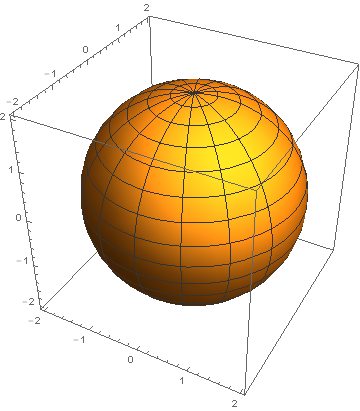
\includegraphics[scale=0.5]{gr-fig-15.png}
		\caption{Surface of a sphere of radius $R=2$}
	\end{figure}
\end{exmp}
But we in fact don't need an extra dimension to describe a curved space. An obvious example is that we don't need to leave the surface of Earth to know that it is curved. With just two coordinates $u$ and $v$ in a 2-dimensional space, we can mathematically show whether the space is curved or not. The first step is to generate tangent vectors:
\begin{align*}
\vec{e}_i = \frac{\partial \vec{r}}{\partial u^i}.
\end{align*} 
For the case of a 2-dimensional surface parameterized by $u$ and $v$, we obtain two tangent vectors:
\begin{align*}
\vec{e}_u = \frac{\partial \vec{S}}{\partial u}, \text{ and } \vec{e}_v = \frac{\partial \vec{S}}{\partial v}.
\end{align*}
Note that these tangent vectors are not in the surface (this is also true in general $n$-dimensional cases). Rather, they lie in a a tangent space $T_p$ at each point $P$ in the space. Tangent vectors are useful because they give directions along the curve or surface.\\

Next, we want to look at an infinitesimal displacement $d\vec{S}$. Because $\vec{S} = \vec{S}(u,v)$, we get from the chain rule:
\begin{align*}
d\vec{S} = \frac{\partial \vec{S}}{\partial u}\,du + \frac{\partial\vec{S}}{\partial v}\,dv = \vec{e}_u\,du + \vec{e}_v\,dv.
\end{align*}
For the sake of convenience (and further generalizations in the future), we shall switch to index notation. Recall that capital Roman characters are reserved for 2-dimensional manifolds, let $u^A = (u^1,u^2) = (u,v)$, with $A=1,2$. This gives
\begin{align*}
d\vec{S} = \vec{e}_A\,du^A.
\end{align*}
It follows that the line element $ds^2$ is
\begin{align*}
ds^2 = d\vec{S}\cdot\,d\vec{S} = \left(\vec{e}_A\,du^A \right) \cdot \left( \vec{e}_B\,du^B\right) = \vec{e}_A \cdot \vec{e}_B\,du^A\, du^B.
\end{align*}
But this is nothing but the all-familiar:
\begin{align*}
\boxed{ds^2 = g_{AB}\,du^A\,du^B}
\end{align*}
Note that we have just shown the above equation holds not only for flat but also for general curved spaces. With this, we can go on to calculate lengths of curves in general curved 2-dimensional spaces. Let a curve in this 2-dimensional space be $\vec{l}(\sigma) = (u(\sigma),v(\sigma))$. The length $L$ is this curve for $a \leq \sigma \leq b$ is given by:
\begin{align*}
L &= \int_{a}^{b}\,ds \\
&= \int_{a}^{b}\sqrt{g_{AB}\,du^A\,du^B}\\ 
&= \int\sqrt{g_{AB}\frac{du^A}{d\sigma}\frac{du^B}{d\sigma}}\,d\sigma\\
&= \int_{a}^{b}\sqrt{g_{AB}\dot{u}^{A}(\sigma)\dot{u}^{B}(\sigma)}\,d\sigma.
\end{align*}
We realize that this has the same form as the length-formula we have found earlier. The only difference is that we are in curved spaces. This suggests that we can generalize this formula for any $n$-dimensional space. \\

We have defined the natural basis vectors as $\vec{e}_A = \partial \vec{S}/\partial u^A$. What about the dual basis vectors? If we try to define the dual basis vectors as $\vec{e}^A = \vec{\nabla}u^A$, we run into trouble. Recall that we had we previous had three coordinates, and that the gradient of $u$ is a normal vector to the surface of constant $u$. However, in 2-dimensional spaces constant $u$ are lines, which has infinitely many normal vectors. This simply means we cannot use the gradient operator to find $\vec{e}^A$. Rather, we will use a more powerful tool, the \textbf{inverse metric tensor}, $g^{AB}$ to raise the index of the natural basis vectors $\vec{e}_A$:
\begin{align*}
\boxed{\vec{e}^A = g^{AB}\vec{e}_B}
\end{align*}
So, the general procedure is: (i) find the tangent vectors, i.e., the natural basis vectors $\vec{e}_A$, (ii) generate the metric tensor $g_{AB}$, (iii) compute the inverse metric tensor $g^{AB}$, and (iv) find the dual basis vectors $\vec{e}^A$ from raising the index of $\vec{e}_A$.\\

\begin{exmp}
	Consider a saddle in 3-dimensional flat space. Using paraboloidal coordinates with constant $w$, find the metric tensor and inverse metric tensor of this saddle surface.\\
	
	Recall the conversion formulas for paraboloidal coordinates:
	\begin{align*}
	x &= u+v\\
	y &= u-v\\
	z &= 2uv
	\end{align*}
	Let be saddle be
	\begin{align*}
	\vec{r} = (u+v, u-v, 2uv).
	\end{align*}
	We first find the tangent vectors (or the natural basis vectors):
	\begin{align*}
	\vec{e}_1 &= \frac{\partial \vec{r}}{\partial u} = (1,1,2v)^\top\\
	\vec{e}_2 &= \frac{\partial \vec{r}}{\partial v} = (1,1,2u)^\top.
	\end{align*}
	Finding the metric tensor is then purely mechanical:
	\begin{align*}
	[g_{AB}] = [\vec{e}_A\cdot\vec{e}_B] = 
	\begin{pmatrix}
	2 + 4v^2 & 4uv\\
	4uv & 2+4u^2
	\end{pmatrix},
	\end{align*}
	as for finding the inverse metric tensor:
	\begin{align*}
	[g^{AB}] = [g_{AB}]^{-1} = 
	\frac{1}{2(1+2u^2+2v^2)}
	\begin{pmatrix}
	1 + 2u^2 & -2uv\\
	-2uv & 1+2v^2
	\end{pmatrix}
	\end{align*}
	With the natural basis vectors and the inverse metric tensor, we can easily find the dual basis vectors:
	\begin{align*}
	\vec{e}^1 = [g^{AB}]\vec{e}_1 &= 
	\frac{1}{2(1+2u^2+2v^2)}
	\begin{pmatrix}
	1 + 2u^2 & -2uv\\
	-2uv & 1+2v^2
	\end{pmatrix}
	\begin{pmatrix}
	1 \\ 1 \\ 2v
	\end{pmatrix}\\
	\vec{e}^2 = [g^{AB}]\vec{e}_2 &= 
	\frac{1}{2(1+2u^2+2v^2)}
	\begin{pmatrix}
	1 + 2u^2 & -2uv\\
	-2uv & 1+2v^2
	\end{pmatrix}
	\begin{pmatrix}
	1 \\ 1 \\ 2u
	\end{pmatrix}
	\end{align*}
\end{exmp}

Ultimately, though, we will find that basis vectors are not so useful once we already have the metric tensor. So we will not be worrying about them so much moving forward. In the next sections, we will explore the Einstein equations, whose purpose is to find the metric tensor describing a space of a given matter distribution. Once we obtain the metric tensor, we can just mechanically work out other characteristics of the space. 

\subsection{Manifolds}
An arbitrary, curved $n$-dimensional space is called a manifold. Assuming that we know the metric tensor, we can write the $n$ coordinates associated with the space as
\begin{align*}
x^a = (x^1, x^2, \dots, x^n),
\end{align*}
for any coordinate system. Next, assume that we have two coordinate systems whose conversion formulae are differential and invertible functions:
\begin{align*}
x^{a'} &= x^{a'}(x^b)\\
x^b = x^b(x^{a'}).
\end{align*}
Next, just like before, we define the Jacobian matrix for the transformation:
\begin{align*}
\boxed{[X^{a'}_b] = \left[\frac{\partial X^{a'}}{\partial X^b}\right]}
\end{align*}
And of course the inverse transformation:
\begin{align*}
\boxed{[X^{a}_{b'}] = \left[\frac{\partial X^{a}}{\partial X^{b'}}\right]}
\end{align*}
These have the usual properties we have seen before:
\begin{align*}
\boxed{X^{a'}_bX^b_{c'} = \delta^a_c = X^{a}_{b'}X^{b'}_c}
\end{align*}
Again, just as before, we define vectors, tensors, and scalars by how the transform:
\begin{empheq}[box=\fbox]{align}
\text{Contravariant vectors: }&\lambda^{a'} = X^{a'}_b\lambda^b \nonumber\\
\text{Covariant vectors: }&\mu_{a'} = X^{b}_{a'}\mu_b
\nonumber\\
\text{Tensors: }&\tensor{\tau}{^{a'b'}_{c'd'}} = X^{a'}_{e}X^{b'}_{f}X^{g}_{c'}X^{h}_{d'}\tensor{\tau}{^{ef}_{gh}}\nonumber\\
\text{Raising/lowering index: } &\tensor{\tau}{^a_b} = g_{bd}\tensor{\tau}{^{ad}}\nonumber\\
\text{Identity: }&g^{ab}g_{bc}=\delta^a_c \nonumber 
\end{empheq}\\

In general, the metric tensor need not be \textbf{positive definite}, which means that $ds^2$ can be positive, negative, or zero. However, the \textbf{signature} (the number of positives minus the number of negatives) of $g_{ab}$ is a scalar and is $-2$ for all metric in general relativity. For instance, $\eta_{\mu\nu}$ has signature $-2$.\\

There are classes of manifolds: \textbf{Riemannian manifolds}, which have positive definite metric tensors, and \textbf{pseudo-Riemannian manifolds}, where metric tensors do not have to be positive definite. Note that spacetime is a pseudo-Riemannian manifold.\\

To define lengths and distances as real numbers, we need to add the absolute values to our previous definitions:
\begin{empheq}[box=\fbox]{align}
\text{Infinitesimal distance: } &ds = \sqrt{\vert\vert g_{ab}\,dx^a\,dx^b \vert\vert} \nonumber \\
\text{Length of a curve: } &L = \int_{a}^{b}\,ds = int^{b}_a\sqrt{\vert\vert g_{ab}\,dx^a\,dx^b \vert\vert} \nonumber \\
\text{Vector norm: } &\vert\vert \vec{\lambda} \vert\vert = \sqrt{\vert\vert \lambda^a \lambda_a \vert\vert} \nonumber
\end{empheq}

Note that vectors can be null or non-null. For non-null vectors in general $n$-dimensional manifolds, we can also define an ``angle'' $\theta$ between two vectors:
\begin{align*}
\cos\theta = \frac{\vec{\lambda}\cdot\vec{\mu}}{\vert\vert \vec{\lambda}\vert\vert \vert\vert \vec{\mu} \vert\vert} = \frac{g_{ab}\lambda^a \lambda^b}{\vert\vert \vec{\lambda}\vert\vert \vert\vert \vec{\mu} \vert\vert}.
\end{align*} 
Beware that this definition works well (intuitively) with positive definite metric tensors. However, for spacetime (whose metric tensor is not positive definite), things can get a little weird. \\

\begin{exmp}
	Consider space-like vector $\lambda^\mu$ in flat 4-dimensional Minkowski spacetime. Find $\theta$ between it and itself.\\
	
	Without changing the inner product (due to invariance), consider a frame where $\lambda^\mu = (0,\vec{\lambda})$. According to our definition:
	\begin{align*}
	\cos\theta = \frac{\eta_{\mu\nu}\lambda^\mu \lambda^\nu}{\vert\vert \lambda^\mu \vert\vert^2} = \frac{-\vert\vert\vec{\lambda}\vert\vert^2}{\vert\vert \vec{\lambda}\vert\vert^2} = -1.
	\end{align*}
	This implies $\theta = \pi$, so the vector makes an angle of $\pi$ with itself. 
\end{exmp}

We call the vectors $\lambda^\mu$ and $\pi^\mu$ \textbf{orthogonal} if $\lambda^\mu\cdot\pi^\mu = 0$, i.e., there exists a frame where they are orthogonal.


\subsection{Tensors on manifolds}
\subsubsection{Combining tensors}
In this section, we will learn the mathematical properties of tensors including special identities and tensor algebra. Familiarizing ourselves with tensor algebra will save us a lot of time and effort when we cover the later topics where we will encounter a few more mathematical objects that are defined on tensors. \\

\begin{prop}
	Adding tensors of the same type gives tensors.
\end{prop}
\begin{proof}
	Let two general tensors $\tensor{\tau}{^{ab}_c}$ and $\tensor{\Theta}{^{ab}_c}$ be given. Let $\tensor{\zeta}{^{a'b'}_{c'}} = \tensor{\tau}{^{a'b'}_{c'}} + \tensor{\Theta}{^{a'b'}_{c'}}$. We will show that $\tensor{\zeta}{^{a'b'}_{c'}}$ is a tensor, i.e.:
	\begin{align*}
	\tensor{\zeta}{^{a'b'}_{c'}} = X^{a}_dX^{b}_eX^f_{c'}\tensor{\zeta}{^{de}_f}.
	\end{align*}
	The proof is a straightforward application of the transformation rules for tensors:
	\begin{align*}
	\tensor{\zeta}{^{a'b'}_{c'}} &= \tensor{\tau}{^{a'b'}_{c'}} + \tensor{\Theta}{^{a'b'}_{c'}} \\
	&= X^{a}_dX^{b}_eX^f_{c'}\tensor{\tau}{^{de}_{f}} + X^{a}_dX^{b}_eX^f_{c'}\tensor{\Theta}{^{de}_{f}}\\
	&= X^{a}_dX^{b}_eX^f_{c'}\left(\tensor{\tau}{^{de}_{f}} +  \tensor{\Theta}{^{de}_{f}}\right) \\
	&= X^{a}_dX^{b}_eX^f_{c'}\tensor{\zeta}{^{de}_{f}}.
	\end{align*}
	Since $\tensor{\zeta}{^{de}_{f}}$ transforms correctly, it is a tensor.
\end{proof}

\begin{prop}
	Multiplying a tensor by a scalar gives a tensor
\end{prop}
\begin{proof}
	The proof to this proposition is trivial. Suppose $\sigma^a_b = \alpha \tau^a_b$, where $\tau^a_b$ is a tensor. We want to show that $\sigma^a_b$ is also a tensor, i.e.,
	\begin{align*}
	\sigma^{a'}_{b'} = X^{a'}_{c}X^d_{b'}\sigma^{c}_d.
	\end{align*}
	Once again, a straightforward application of the transformation rule applies:
	\begin{align*}
	\sigma^{a'}_{b'} &= \alpha\tau^{a'}_{b'}\\
	&= \alpha X^{a'}_{c}X^d_{b'}\tau^{c}_{d}\\
	&= X^{a'}_{c}X^d_{b'} \sigma^{c}_d.
	\end{align*}
\end{proof}

So far, we have seen that properties of tensors are similar to those of vectors. Specifically, we see that tensor spaces, similar to vector spaces, are also closed under addition and scalar multiplication. But there are more properties that tensor spaces have but vector spaces do not.

\begin{prop}
	Products of tensors are tensors.
\end{prop}
\begin{proof}
	Suppose that $\tensor{\sigma}{^{ab}_c} = \lambda^a \tensor{\tau}{^b_c}$. We want to show:
	\begin{align*}
	\tensor{\sigma}{^{a'b'}_{c'}} = X^{a'}_{d}X^{b'}_{e}X^{f}_{c'}\tensor{\sigma}{^{de}_f}
	\end{align*}
	Once again...
	\begin{align*}
	\tensor{\sigma}{^{a'b'}_{c'}} &= \lambda^{a'}\tensor{\tau}{^{b'}_{c'}}\\
	&= \left(X^{a'}_d \lambda^d \right) \left( X^{b'}_eX^f_{c'}\tensor{\tau}{^e_f}\right) \\
	&= X^{a'}_dX^{b'}_eX^f_{c'}\lambda^d\tensor{\tau}{^e_f}\\
	&= X^{a'}_{d}X^{b'}_{e}X^{f}_{c'}\tensor{\sigma}{^{de}_f}
	\end{align*}
\end{proof}

\begin{prop}
	Contracting a tensor of type $(r,s)$ gives a tensor of type $(r-1,s-1)$.
\end{prop}
\begin{proof}
	Suppose $\tensor{\tau}{^{ab}_{cd}}$ is a $(2,2)$ tensor. Let us call another tensor $\sigma^{a}_b = \tensor{\tau}{^{ab}_{cb}}$, which is a $(1,1)$ tensor. We want to show that the contraction $\sigma^{a}_{b}$ is also a tensor:
	\begin{align*}
	\sigma^{a'}_{b'} = X^{a'}_{d}X^{g}_{b}\sigma^{d}_g.
	\end{align*}
	Again, applying the transformation rules:
	\begin{align*}
	\sigma^{a'}_{b'} &= \tensor{\tau}{^{a'c'}_{c'b'}}\\
	&= X^{a'}_{d}X^{c'}_{e'}X^{f}_{c'}X^{g}_{b'}\tensor{\tau}{^{dc}_{fg}}\\
	&= X^{a'}_{d}X^{g}_{b'}\delta^{e}_f\tensor{\tau}{^{de}_{fg}}\\
	&= X^{a'}_{d}X^{g}_{b'}\tensor{\tau}{^{de}_{eg}}\\
	&= X^{a'}_{d}X^{g}_{b'}\sigma^{d}_g.
	\end{align*}
\end{proof}
Note that we have already seen this property already in the index lowering/raising operations. For example:
\begin{align*}
\lambda_a = g_{ab}\lambda^b.
\end{align*}
As a consequence of the above proposition, we can let $\tensor{\sigma}{^{ab}_{c}}$ be
\begin{align*}
\tensor{\sigma}{^{ab}_{c}} = \tensor{\tau}{^{abe}}\mu_eg_{cf}\lambda^f,
\end{align*}
and know immediately that it is a tensor (since the indices ``add up to'' or ``contract to'' to upper $ab$ and lower $c$).

\begin{prop}[Diving: Quotient Theorem]
	Suppose $\tensor{\tau}{^{a}_{bc}}\lambda^c$ transforms as a tensor for all $\lambda^c$. The \textbf{quotient theorem} says $\tensor{\tau}{^{a}_{bc}}$ is a tensor.  
\end{prop} 
\begin{proof}
	We want to show that 
	\begin{align*}
	\tensor{\tau}{^{a'}_{b'g'}} = X^{a'}_dX^{e}_{b'}X^{f}_{g'} \tensor{\tau}{^d_{ef}}.
	\end{align*}
	We first know that the given quantity transforms correctly as a tensor. We also know that $\lambda^{c'} = X^{c'}_f\lambda^f$. It follows that
	\begin{align*}
	\tensor{\tau}{^{a'}_{b'c'}}\left( X^{c'}_f\lambda^f \right) - X^{a'}_dX^{e}_{b'}\tensor{\tau}{^d_{ef}}\lambda^f &= 0\\
	\tensor{\tau}{^{a'}_{b'c'}}X^{c'}_f - X^{a'}_dX^{e}_{b'}\tensor{\tau}{^d_{ef}} &= 0\\
	\tensor{\tau}{^{a'}_{b'c'}}X^{c'}_f &= X^{a'}_dX^{e}_{b'}\tensor{\tau}{^d_{ef}}\\
	\tensor{\tau}{^{a'}_{b'c'}}\delta^{c'}_{g'} &= X^{a'}_dX^{e}_{b'}X^{f}_{g'}\tensor{\tau}{^d_{ef}}\\
	\tensor{\tau}{^{a'}_{b'g'}}&=X^{a'}_dX^{e}_{b'}X^{f}_{g'}\tensor{\tau}{^d_{ef}}.
	\end{align*}
	Therefore, $\tensor{\tau}{^{a}_{bc}}$ is a tensor. 
\end{proof}

\subsubsection{Special tensors}
\textbf{Symmetric tensors}. Let a two-indexed tensor $\tau_{ab}$ be given. It is symmetric if
\begin{align*}
\tau_{ab} = \tau_{ba}.
\end{align*}
Note that a straightforward application of the transformation rule can show that if a tensor is symmetric in one frame $(S)$, then it is also symmetric in a different frame $(S')$.\\

\noindent \textbf{Anti-symmetric tensors}. Let a 2-indexed tensor $\tau^{ab}$ be given. We say that $\tau_{ab}$ is anti-symmetric if
\begin{align*}
\tau_{ab} = -\tau^{ba}.
\end{align*}
Again, an application of the transformation rule can show that if a tensor is anti-symmetric in one frame, it is anti-symmetric in all frames. \\

\noindent \textbf{Kronecker delta}. Recall that the Kronecker delta (a type $(1,1)$ tensor) is defined as
\begin{align*}
\delta^a_b = \begin{cases*}
1, a=b\\
0, a\neq b.
\end{cases*}
\end{align*}
As we might have seen before, the Kronecker delta is frame-independent:
\begin{align*}
\delta^{a}_b =X^{a'}_{e}X^{f}_{b'}\delta^{e}_f = X^{a'}_eX^e_{b'} =\delta^{a'}_{b'}.
\end{align*}

\noindent \textbf{Note:} For most tensors (with any arbitrary number of indices), the ordering of indices matter, i.e., $\tensor{\tau}{^{abe}} \neq \tensor{\tau}{^{aeb}}$ in general. Therefore, if we are not sure whether the ordering of the indices matter, we should not write, for instance $\tau^{ac}_b$ because this could mean, say $\tensor{\tau}{^a_c^b}$ or $\tensor{\tau}{^{ac}_b}$. 
	 

\newpage

\section{Gravitation and Curvature}
As we have said many times before, in general relativity, gravity is not a force. Rather, matter (mass and energy) causes spacetime to curve. And because gravity is not a force, we define \textbf{free particles} - objects who are not acted upon by any force - as objects moving with no forces \textbf{other than gravity}. The trajectory of free particles are called \textbf{geodesics}. \\

In this section, we will learn about:
\begin{itemize}
	\item Curvature: How can we tell if a space is curved?
	\item Geodesics: What is an equation to solve for a geodesic, and how can we solve for a geodesic?
	\item Motion in curved spaces: How do vectors behave as we move them along a geodesic? What if we move them not along a geodesic?
	\item The laws of physics: How do we describe the laws of physics in tensor form? As space can be curved and vectors can change due to the curvature of space, how we define the ``derivative?''
	\item Newtonian limit: Will we be able to get back Newtonian physics in the limit?
\end{itemize}
This section will provide us with some powerful mathematical machinery for working with and understanding the Einstein equations and cosmology in the future.
\subsection{Curvature}
As tiny humans living of the surface of a giant ball, how could we tell that the space we are living in, where it seems locally flat, is actually curved? And what we mean by ``going straight'' once we have found out the Earth is round?\\

One way to test if a 2-dimensional space (the Earth for instance) is to just to walk, but with equal left and right step lengths. Have two people start walking parallel to each other. If one point their paths cross, then the space is curved.\\

Another way to see if the Earth is curved or flat is doing the ``triangle test.'' Simply generated a ``spherical triangle'' on the surface of Earth by intersecting three \textbf{great circles} (so the equator and two perpendicular (at the pole) longitude lines would suffice). We would observe that the sum of the angles in this triangle is $270^\circ$, not $180^\circ$. This says that the surface of the Earth is curved.\\

Now, before we go on and attempt to make a rigorous procedure to distinguish curved and flat spaces, we should make a few key observations this above example: 
\begin{itemize}
	\item If parallel lines cross in a space, then the space is non-Euclidean and is therefore curved. 
	\item Lines formed when walking ``straight'' (walking with left step size equal right step size as in our first method) are geodesics. 
	\item On a sphere, great circles are circles whose center is the origin, for example: the equator, longitude lines. Beware that latitude lines are not great circles. On a sphere, great circles are geodesics. 
	\item 
\end{itemize}

\subsection{Geodesics and Affine connections $\Gamma^{\sigma}_{\mu\nu}$}
In this section, we will learn a procedure to generate a geodesic, given that we are in a space or spacetime where we know the metric of the space. This procedure will follow something along the line of ``moving straight'' in the space, but much more mathematically rigorous.\\

\subsubsection{Flat 3D space}
Let us consider the simplest possible case with flat 3D case where geodesics are, as we guessed it, literally straight lines. In Cartesian coordinates, a straight line obeys the ``no-curvature'' equation:
\begin{align*}
\frac{\partial^2 \vec{r}}{\partial t^2} = \vec{0}.
\end{align*}
Now, suppose that we are in an arbitrary curvilinear coordinate system. What would be the equation of a straight line here? It makes sense to think about \textbf{distance} and \textbf{displacement}. If we are moving such that the distance covered the same as displacement, at every instance, then we are moving in a straight line. So, let our displacement be $\vec{r}$. With arc length parameterization: $\vec{r} = \vec{r}(s)$, where $s$ is essentially distance traveled. The condition of straightness gives:
\begin{align*}
\boxed{\left|\left| \dot{\vec{r}}(s) \right|\right| = \left|\left| \frac{d\vec{r}}{ds} \right\|\right| = 1 }
\end{align*}
We should recognize that $d\vec{r}/ds$ is nothing but the tangent vector to the path. Let's call this vector $\vec{\lambda}$. Using the chain rule, it follows that
\begin{align*}
\vec{\lambda} = \frac{d\vec{r}}{ds} = \frac{\partial \vec{r}}{\partial u^i}\frac{\partial u^i}{\partial s} = \frac{\partial u^i}{\partial s}\vec{e}_i = \lambda^i\vec{e}_i,
\end{align*}
where $u^i$ is simply a coordinate in the curvilinear coordinate system. The above equality gives:
\begin{align*}
\boxed{\lambda^i = \frac{\partial u^i}{\partial s} = \dot{u}^i(s)}
\end{align*}
Now, be $\vec{\lambda}$ is a tangent vector, its direction does not change along a straight line. Since we also know that $\vert\vert \vec{\dot{r}}(s) \vert\vert = 1$, $\vec{\lambda}$ has both fixed direction and magnitude along a straight line. Therefore, ``straightness,'' at least in this limited case, implies that the derivative of tangent vectors with respect to arc length is zero. We call this implication the \textbf{condition of straightness}:
\begin{align*}
\boxed{\frac{\partial \vec{\lambda}}{\partial s} = 0}
\end{align*}
Let's take a closer look at the boxed expression but in a different coordinate system. If we think about the above equality, it should also make sense for any general 3-dimensional coordinate system in flat space, in which case:
\begin{align*}
\frac{d}{ds}\left(\lambda^i \vec{e}_i \right) = \dot{\lambda^i}\vec{e}_i + \lambda^i\dot{\vec{e}}_i  =  \vec{0}. 
\end{align*}
In Cartesian coordinates, the basis vectors $\vec{e}_i$ happen to be constant, so $\dot{\vec{e}}_i = \vec{0}$. This gives $\dot{\lambda}^i = 0$. And since $\lambda^i = \dot{u}^i = \dot{x}^i$, which implies $\partial^2 x^i/\partial s^2 = \vec{0}$. Now imagine if we parameterize $\vec{r}$ with a different parameter, say $t$. If $t \propto s$, then
\begin{align*}
\frac{\partial^2 x^i}{\partial s^2} = \frac{\partial x^2 x^i}{\partial t} = \vec{0}
\end{align*}
holds. This is equivalent to the case we have an object moving with constant velocity (so that $s = vt$). If $s$ is not proportional to $t$ then the above equality does not hold.\\

We have established the ``condition of straightness'' in Cartesian coordinates. However, the equation $\partial^2 x^i/\partial s^2 = 0$ does not hold for general coordinate systems. Rather, the more fundamental equation applies:
\begin{align*}
\boxed{\frac{\partial \lambda^i}{\partial s}\vec{e}_i + \lambda^i\frac{\partial \vec{e}_i}{\partial s} = 0}
\end{align*}
where 
\begin{align*}
\frac{\partial \vec{e}_i}{\partial s} = \frac{\partial \vec{e}_i}{\partial u^j}\frac{\partial u^j}{\partial s}  = \frac{\partial \vec{e}_i}{\partial u^j}\dot{u}^j \neq 0
\end{align*}
in general. Now, to simplify our notation, let us use (as we have introduced before) $\partial_j = \partial/\partial u^j$. This gives:
\begin{align*}
\frac{\partial \lambda^i}{\partial s}\vec{e}_i + \lambda^i\frac{\partial \vec{e}_i}{\partial s} 
=  \dot{\lambda}^i\vec{e}_i + \lambda^i\left( \partial_j \vec{e}_i\right)\dot{u}^j 
=0
\end{align*} 
Note that $\partial_j\vec{e}_i$ are vectors, which we can expand in terms of basis vectors, but we will not do that. Rather, let us define the \textbf{Christoffel symbol}, or the \textbf{affine connection}, $\Gamma^{k}_{ij}$ in terms of $\partial_j\vec{e}_i$ as:
\begin{align*}
\boxed{\partial_j\vec{e}_i = \Gamma^{k}_{ij}\vec{e}_k}
\end{align*}
We will interpret $\Gamma^{k}_{ij}$ as ``the $k^{\text{th}}$ component of the $u^{j\,\text{th}}$ derivative of $\vec{e}_i$.'' It is very important that we keep in mind $\Gamma^{k}_{ij}$ is \textbf{not} a tensor. Rather, the Christoffel symbols are \textbf{connections} - they are just vector components.\\

With the definition of $\Gamma^{k}_{ij}$, we can express the derivative of $\vec{e}_i$ as:
\begin{align*}
\dot{\vec{e}}_i = \left(\partial_j\vec{e}_i \right)\dot{u}^j = \Gamma^{k}_{ij}\vec{e}_k\dot{u}^j. 
\end{align*}
It follows that the condition of straightness becomes:
\begin{align*}
\frac{d\vec{\lambda}}{ds} &= \dot{\lambda}^i\vec{e}_i + \lambda^i \Gamma^{k}_{ij}\vec{e}_k\dot{u}^j\\
&= \dot{\lambda}^i\vec{e}_i + \lambda^j \Gamma^{i}_{jk}\vec{e}_i\dot{u}^k, \text{ letting $i\rightarrow j, j\rightarrow k, k \rightarrow i$}\\
&= \left(\dot{\lambda}^i + \Gamma^{i}_{jk}\dot{u}^k \right)\vec{e}_i\\
&= 0, 
\end{align*}
or
\begin{align*}
\dot{\lambda}^i + \Gamma^{i}_{jk}\dot{u}^k = 0.
\end{align*}
Let us write the above equality more completely with the arc length parameter $s$, and call it the equation of a straight line in flat 3-dimensional space. But notice how the number of dimensions do not really play a role anywhere in our derivation. This hints to us that the equation also holds for $n$-dimensional manifolds, but we will discuss this topic later on.
\begin{align*}
\boxed{\frac{d^2u^i}{ds^2} + \Gamma^{i}_{jk}\frac{du^j}{ds}\frac{du^k}{ds} = 0}
\end{align*}
For $i,j,k$, the above expressions encodes $3$ equations whose solution is geodesic in flat space.\\ 

Now, let us ``worry'' a little bit about the Christoffel symbol $\Gamma^{i}_{jk}$. It seems like that because $\Gamma^{i}_{jk}$ has three indices $i,j,k$, there will be $27$ coefficients associated with different combinations of $i,j,k$. However, we can show that this is not the case. Recall that
\begin{align*}
\partial_j \vec{e}_i = \Gamma^{k}_{ij}\vec{e}_k.
\end{align*}
Dotting the entire equation with $\vec{e}^l$ gives
\begin{align*}
\partial_j \vec{e}_i\cdot\vec{e}^l = \Gamma^{k}_{ij}\vec{e}_k\cdot\vec{e}^l = \Gamma^{k}_{ij}\delta^l_k = \Gamma^{l}_{ij}.
\end{align*}
Also, observe that 
\begin{align*}
\partial_j\vec{e}_i = \frac{\partial }{\partial u^j}\frac{\partial \vec{r}}{\partial u^i} = \frac{\partial }{\partial u^i}\frac{\partial \vec{r}}{\partial u^j} = \partial_i\vec{e}_j.
\end{align*}
This simply implies a symmetric relation:
\begin{align*}
\boxed{\Gamma^{l}_{ij} = \Gamma^{l}_{ji}}
\end{align*}
So, it turns out that we only  have $18$ independent terms, instead of $27$.\\

Next, we want to the relationship between the Christoffel symbols and the metric tensor. Specifically, we want to find out how to compute the Christoffel symbols, using the metric tensor. Consider:
\begin{align*}
\partial_k g_{ij} &= \partial_k\left(\vec{e}_i\cdot\vec{e}_j \right) \\
&= \vec{e}_j\partial_k\vec{e}_i + \vec{e}_i\partial_k\vec{e}_j\\
&= \vec{e}_j \Gamma^{m}_{ik}\vec{e}_m + \vec{e}_i\Gamma^{m}_{kj}\vec{e}_m.
\end{align*}
This gives
\begin{align*}
\boxed{\partial_k g_{ij} = \Gamma^{m}_{ik}g_{jm} + \Gamma^{m}_{jk}g_{im}}
\end{align*}
By symmetry, we also get
\begin{align*}
\boxed{\partial_i g_{jk} = \Gamma^{m}_{ji}g_{km} + \Gamma^{m}_{ki}g_{jm}}
\end{align*}
and
\begin{align*}
\boxed{\partial_j g_{ik} = \Gamma^{m}_{kj}g_{im} + \Gamma^{m}_{ij}g_{km}}
\end{align*}
Adding the first two equations and subtract the third, we get
\begin{align*}
\partial_k g_{ij} + \partial_i g_{jk} - \partial_j g_{ik} = 2\Gamma^{m}_{ik}g_{jm}.
\end{align*}
Next, multiplying this entire equation by $g_{jl}$, so that $g_{jm}g^{jl} = \delta^l_m$, we get
\begin{align*}
\Gamma^{l}_{ik} = \frac{1}{2}g^{jl}\left( \partial_k g_{ij} + \partial_i g_{jk} - \partial_j g_{ik}\right).
\end{align*}
Finally, letting $l\rightarrow k, k\rightarrow i, i\rightarrow j, j\rightarrow l $, we obtain the formula to compute the Christoffel symbol from the metric:
\begin{align*}
\boxed{\Gamma^{k}_{ij} = \frac{1}{2}g^{kl}\left( \partial_i g_{jl} + \partial_j g_{il} - \partial_l g_{ij}\right)}
\end{align*}
Now, in Cartesian coordinates, the metric is simply the identity matrix, which is constant. This simply means that all Christoffel symbols $\Gamma^{k}_{ij}$ in Cartesian coordinates are zero. However, this does not imply if the Christoffel symbols are non-zero then the space is curved. In fact, we get non-zero Christoffel symbols in curvilinear coordinates in flat space whenever the basis vectors $\vec{e}_i$ are not constant. An example would be spherical coordinates, which we will soon find out.\\

We might ask whether there is a nice, short way to calculate the Christoffel symbols. Unfortunately, the answer is no - brute force is the only way to go. Luckily, though, Mathematica can handle Christoffel symbol computations, given a metric tensor. 
\begin{exmp}
	Find $\Gamma^{1}_{23} = \Gamma^1_{32}$.\\
	
	Again, brute force is the way to go:
	\begin{align*}
	\Gamma^{1}_{23} &= \Gamma^1{32}\\
	&= \frac{1}{2}g^{11}\left( \partial_2 g_{31} + \partial_3 g_{21} - \partial_1 g_{23}\right)\\
	&+ \frac{1}{2}g^{12}\left( \partial_2 g_{32} + \partial_3 g_{22} - \partial_2 g_{23}\right)\\
	&+
	\frac{1}{2}g^{13}\left( \partial_2 g_{33} + \partial_3 g_{23} - \partial_3 g_{23}\right)
	\end{align*}
	We can of course repeat this process to find the other 25 terms, but we will not do that!
\end{exmp}

We have used arc length as a parameter in finding the geodesic equation:
\begin{align*}
\frac{d^2u^i}{ds^2} + \Gamma^{i}_{jk}\frac{du^j}{ds}\frac{du^k}{ds} = 0.
\end{align*}
Now, what if we use a different parameter $t = f(s)$? How will the form of the equation above change? We can show (but we won't) that with $t = f(s)$, the above equation has an extra term:
\begin{align*}
\boxed{\frac{d^2u^i}{ds^2} + \Gamma^{i}_{jk}\frac{du^j}{ds}\frac{du^k}{ds} = -\frac{d^2t}{ds^2}\left( \frac{dt}{ds}\right)^{-2}\frac{du^i}{dt}}
\end{align*}
But if we have a linear relationship between $t$ and $s$, i.e.,
\begin{align*}
t = As +B,
\end{align*}
where $A\neq 0$ and $B$ are constants, then we get
\begin{align*}
\boxed{\frac{d^2u^i}{dt^2} + \Gamma^{i}_{jk}\frac{du^j}{dt}\frac{du^k}{dt} = -\frac{d^2t}{ds^2}\left( \frac{dt}{ds}\right)^{-2}\frac{du^i}{dt} = 0}
\end{align*}
simply because
\begin{align*}
\frac{d^2t}{ds^2} = 0.
\end{align*}
A parameter $t$ of this form $t = As + B$ is called an \textbf{affine parameter}. 

\subsection{Geodesics in curved space}
We have seen multiple correspondences between flat 3-dimensional space in curvilinear coordinates and curved general $N$-dimensional manifolds:
\begin{align*}
u^j &\leftrightarrow x^a\\
g_{ij} &\leftrightarrow g_{ab}\\
\lambda^{i'} = U^{i'}_j\lambda^j &\leftrightarrow \lambda^{a'}X^{a'}_b\lambda^b\\
ds^2 = g_{ij}\,du^i\,du^j &\leftrightarrow ds^2 = g_{ab}\,du^a\,du^b,
\end{align*} 
which is not surprising because flat 3-dimensional space is simply a special case of general curved $N$-dimensional spaces. We have expected the form of the geodesic equation in flat 3-dimensional space to remain the same in general curved $N$-dimensional space. And we should be correct, because nowhere in our derivation of the geodesic equation is dimension-specific, i.e., the derived equation does not just apply exclusively to the flat three dimensional case. So, the geodesic equation in general curved $N$-dimensional space is simply
\begin{align*}
\boxed{\frac{d^2x^a}{d\sigma^2} + \Gamma^{a}_{bc}\frac{dx^b}{d\sigma}\frac{dx^c}{d\sigma} = 0}
\end{align*} 
where $\sigma$ is an \textbf{affine parameter}. The Christoffel symbol $\Gamma^{a}_{bc}$ is defined in exactly the same fashion as before:
\begin{align*}
\boxed{\Gamma^{a}_{bc} = \frac{1}{2}g^{ad}\left( \partial_b g_{cd} + \partial_c g_{bd} - \partial_d g_{bc}\right)}
\end{align*}
Now, let us dwell into a nice example that illustrates how the geodesic equation gives a geodesic. 
\begin{exmp}
	Determine if lines of constant latitude of a 2-sphere of radius $a$ are geodesics.\\
	
	We have said before that only great circles on a sphere are geodesics. Now, we can verify this fact using the geodesic equation. First, consider any circle on the 2-sphere of radius $2$. Let us oriented the sphere so that this line is the line of constant latitude. 
	\begin{align*}
		\text{insert figure 16 here!!!}
	\end{align*}
	Next, let us gather all we have known about the geometry of a 2-sphere. The metric tensor is given by
	\begin{align*}
	[g_{AB}] = \begin{pmatrix}
	a^2 & 0 \\
	0 & a^2\sin^2\theta
	\end{pmatrix},
	\end{align*}
	and the inverse metric tensor is given by
	\begin{align*}
	[g^{AB}] = \begin{pmatrix}
	a^{-2} & 0\\
	0 & a^{-2}\sin^{-2}\theta
	\end{pmatrix},
	\end{align*}
	where $\theta$ is the angle form by the position vector $\vec{r}$ with the $z$-axis. The line of constant latitude is given by the parameters:
	\begin{align*}
	u^A = (u^1,u^2) = (\theta,\phi),
	\end{align*}
	where $\theta$ is fixed and $0 \leq \phi \leq 2\pi$. The question we should be asking ourselves is whether
	\begin{align*}
	\frac{d^2u^A}{ds^2} + \Gamma^{A}_{BC}\frac{du^B}{ds}\frac{du^C}{ds} = 0,
	\end{align*}
	where $s$ is the arc length parameter, holds for certain values of $\theta$. Because lines of constant latitudes are circles, the arc length $s$ is easy to find: $s(\phi) = r'\phi = a\phi\sin\theta$. This gives:
	\begin{align*}
	\phi = \frac{s}{a\sin\theta}.
	\end{align*}
	Therefore, we can parameterize the path with the arc length $s$:
	\begin{align*}
	u^A(s) = (u^1,u^2)(s) = \left(\theta, \frac{s}{a\sin\theta}\right).
	\end{align*}
	But since $\theta$ is fixed,
	\begin{align*}
	\frac{d^2u^A}{ds^2} = (0,0).
	\end{align*}
	So it seems that we only need to check for which $\theta$
	\begin{align*}
	\Gamma^{A}_{BC}\frac{du^B}{ds}\frac{du^C}{ds} = 0.
	\end{align*}
	So the next reasonable step to take is computing the Christoffel symbols. There are 8 of these, but it turns out (by symmetry and the fact that $g_{AB}$ is diagonal), we only have to do a few computations:
	\begin{align*}
	\Gamma^1_{22} &= -\sin\theta\cos\theta\\
	\Gamma^2_{12} &= \Gamma^2_{21} = \cot\theta\\
	\Gamma^1_{12} &= \Gamma^1_{21} = \Gamma^2_{11} = \Gamma^2_{22} = 0.
	\end{align*}
	For $A = 1$, 
	\begin{align*}
	\Gamma^{A}_{BC}\frac{du^B}{ds}\frac{du^C}{ds} &= 0\\
	\Gamma^{1}_{BC}\frac{du^B}{ds}\frac{du^C}{ds} &= 0\\
	-\sin\theta\cos\theta\frac{du^2}{ds}\frac{du^2}{ds} &= 0\\
	-\sin\theta\cos\theta\left(a\sin\theta \right)^{-2} &= 0
	\end{align*}
	can only be true if $\theta = \pi/2$. This suggests that the equator is the only viable candidate to be a geodesic. However, we should check if the equality can hold for $A=2$, because if the equality cannot hold then we have to conclude that lines of constant latitude cannot be geodesics. Let us check:
	\begin{align*}
	\Gamma^{A}_{BC}\frac{du^B}{ds}\frac{du^C}{ds} &= 0\\
	\Gamma^{2}_{BC}\frac{du^B}{ds}\frac{du^C}{ds} &= 0\\
	(0+0)\cot\theta &= 0.
	\end{align*}
	Ah! So equality holds are any $\theta$ in this case. Combining the above too facts, we conclude that only the circle of latitude $\pi/2$ works as a geodesic. Equivalently, for a sphere, only great circles are geodesics.
\end{exmp}
\subsection{Parallel transport}
Our condition for constructing a geodesic was that the tangent vector $\vec{\lambda} = \lambda^i\vec{e}_i = \lambda_i = \vec{e}^i = \dot{u}^i\vec{e}_i$ does not change as we move along the curve, i.e. the condition of straightness:
\begin{align*}
\frac{d\vec{\lambda}}{ds} = 0,
\end{align*} 
which led us to the geodesic equation:
\begin{align*}
\ddot{u}^i + \Gamma^i_{jk}\dot{u}^j\dot{u}^k = 0.
\end{align*}
Now, what about any arbitrary vector $\vec{\lambda}$ that is not a tangent to the geodesic? To ask how $\vec{\lambda}$ changes as it moves along a geodesic is a legitimate question. However, we have to be more specific. There are infinitely many ways for $\vec{\lambda}$ to travel along the geodesic because the ``tangent condition'' is no longer required. So, let us require that we move $\vec{\lambda}$ along the geodesic in such a way that the only changes happening the $\vec{\lambda}$ are due to the geometry of the space. For instance, imagine pushing a pencil along the equator without rotating it. Obviously the direction of the pencil changes over time, but not because we are exerting a torque on it but rather because the surface of the globe is a curved space. We this action of ``moving a vector in a space without changing it'' \textbf{parallel transport}. We will define this term more rigorously as we move on. \\

Now, because $\vec{\lambda}$ does not change. Let $t$ be an affine parameter, we get the \textbf{condition of parallel transport}:
\begin{align*}
\frac{d\vec{\lambda}}{dt} = 0.
\end{align*}  
In flat space, $\vec{\lambda}$ does not change its direction due to parallel transport. But in curved spaces, as we have discussed in the example of the pencil and the globe, $\vec{\lambda}$ can change directions due to curvature. Now, we can expand the condition of parallel transport to get further insights:
\begin{align*}
\frac{d\vec{\lambda}}{dt} &= 0\\
\dot{\lambda}^i \vec{e}_i + \lambda^i\vec{e}^{\,i} &= 0.
\end{align*}
Since we also know that
\begin{align*}
\dot{\vec{e}}_i = \dot{u}^j\partial_j\vec{e}_i = \Gamma^k_{ij}\dot{u}^j\vec{e}_k,
\end{align*}
letting $k\rightarrow i, i \rightarrow j, j \rightarrow k$, we get
\begin{align*}
\dot{\lambda}^i + \lambda^j \Gamma^i_{kj}\dot{u}^k = 0
\end{align*}
This equation tells us how the components $\lambda^i$ change when $\vec{\lambda}$ is parallel transported along any curve parameterized by the affine parameter $t$. Note (again) that our geodesic equations are not dimension-specific, i.e., we can just change the indices for the equation to work in any $N$-dimensional manifold:
\begin{align*}
\boxed{\dot{\lambda}^a + \lambda^b \Gamma^a_{bc}\dot{u}^c = 0}
\end{align*}

\begin{exmp}
	Show that we get the geodesic equation from the above equality in the case where $\vec{\lambda}$ is a tangent vector.\\
	
	If $\lambda^i = \dot{u}^i$, then the above equality simply becomes:
	\begin{align*}
	\ddot{u}^i + \Gamma^i_{jk}\dot{u}^j\dot{u}^k = 0,
	\end{align*}
	which is exactly the geodesic equation. Note that this also says to parallel transport tangent vectors, the curve must be a geodesic (so that $\vec{\lambda}$ remains a tangent vector). 
\end{exmp}

\begin{exmp}
	Consider a unit vector $\vec{\lambda}$ on the surface of a sphere of radius $a$ which makes an angle $\alpha$ with respect to a longitude line. 
	\begin{align*}
	\text{insert figure 17 here!!!}
	\end{align*}
	Show that as $\vec{\lambda}$ is parallel transported along the line of constant latitude $\theta_0$, the direction of $\vec{\lambda}$ changes by an angle $\chi = 2\pi \omega$, where $\omega = \cos\theta_0$. \\
	
	First, we parameterize the curve as $u^A = (u^1,u^2) = (\theta_0, \phi)$, where $\theta_0$ is fixed and $0 \leq \phi \leq 2\pi$. The arc length is $s = \phi a\sin\theta_0$. So this gives, as before, $\phi = s\left(a\sin\theta_0 \right)^{-1}$. Next, let $\vec{\lambda}(0)$ be the vector before parallel transport and $\vec{\lambda}(2\pi)$ be the vector after parallel transport. We know that $\chi$ is the angle between formed between these two vectors. Now, because $\vec{\lambda}(0)$ makes an angle $\alpha$ with a longitude line, we have
	\begin{align*}
	\lambda^A(0) = \left( \lambda^1(0),\lambda^2(0)\right) = \left(a^{-1}\cos\alpha, \left( a\sin\theta_0\right)^{-1}\sin\alpha  \right).
	\end{align*}
	We can readily verify that $\vec{\lambda}(0)$ is indeed a unit vector:
	\begin{align*}
	&\text{ }g_{AB}\lambda^A(0)\lambda^B(0)\\
	 &= 
	\begin{pmatrix}
	a^{-1}\cos\alpha & \left(a\sin\theta_0 \right)^{-1}\sin\alpha 
	\end{pmatrix}
	\begin{pmatrix}
	a^2 & 0\\
	0 & \left(a\sin\theta_0 \right)^2 
	\end{pmatrix}
	\begin{pmatrix}
	a^{-1}\cos\alpha\\
	\left( a\sin\theta_0\right)^{-1}\sin\alpha 
	\end{pmatrix}\\
	&=
	\cos^2\alpha + \sin^2\alpha = 1.
	\end{align*}
	We can also readily verify that $\lambda^A(0)$ makes an angle $\alpha$ with the longitude line. Let $\mu^A$ be a vector that points along a longitude line. In Cartesian coordinates, 
	\begin{align*}
	\mu^A = 1 \vec{e}_{\theta} + 0\vec{e}_\phi.
	\end{align*} 
	So, in the spherical basis, $\mu^A$ simply becomes $(1,0)^\top$. The angle between $\lambda^A$ and $\mu^A$ can come out of their inner product:
	\begin{align*}
	\cos\beta = \frac{g_{AB}\mu^A\lambda^B}{\vert\vert \mu^A \vert\vert \vert\vert \lambda^B\vert\vert} = \frac{a^2a^{-1}\cos\alpha}{a} = \cos\alpha.
	\end{align*}
	So, the angle between $\mu^A$ and $\lambda^A$ is indeed $\alpha$. Next, we parallel transport $\lambda^A$ along the line of constant latitude $\theta_0$. We need to solve the parallel transport equations (there will be two of them) to find the new components of $\vec{\lambda}$ after parallel transporting:
	\begin{align*}
	\dot{\lambda}^A + \Gamma^A_{BC}\lambda^B\dot{u}^C = 0.
	\end{align*}
	With initial values
	\begin{align*}
	\vec{\lambda}(0) = 
	\begin{pmatrix}
	a^{-1}\cos\alpha\\
	\left(a\sin\theta_0 \right)^{-1}\sin\alpha 
	\end{pmatrix},
	\end{align*}
	the problem boils down to an ordinary differential initial value problem. Using the Christoffel symbols we have found before, we have a coupled system of equations:
	\begin{align*}
	\begin{cases*}
	\dot{\lambda}^1 + \Gamma^1_{22}\lambda^2 \dot{u}^2 = 0\\
	\dot{\lambda}^2 + \Gamma^2_{12}\lambda^1\dot{u}^1 + \Gamma^2_{21}\lambda^2\dot{u}^2= 0
	\end{cases*}.
	\end{align*}
	We are not going over the details of how to solve this system, but we certain verify that 
	\begin{align*}
	\lambda^A(t) &= \left( \lambda^1(t),\lambda^2(t)\right)\\
	&= \left(a^{-1}\cos(\alpha-\omega t), \left( a\sin\theta_0\right)^{-1}\sin(\alpha-\omega t)  \right)  
	\end{align*}
	where $\omega = \cos\theta_0$ solves the initial value problem. Now, let $t = 2\pi$, we get
	\begin{align*}
	\lambda^A(2\pi) = \left(a^{-1}\cos(\alpha - 2\pi\omega) , \left(a\sin\theta_0 \right)^{-1}\sin(\alpha-2\pi\omega)  \right). 
	\end{align*}
	The final step is to find the angle between $\lambda^A(0)$ and $\lambda^A(2\pi)$:
	\begin{align*}
	\cos\chi &= \frac{g_{AB}\lambda^A(0)\lambda^B(2\pi)}{\vert\vert \lambda^A(0)\vert\vert\vert\vert \lambda^B(2\pi)\vert\vert} = \frac{g_{AB}\lambda^A(0)\lambda^B(2\pi)}{1}\\
	&= a^2a^{-1}\cos\alpha a^{-1}\cos(\alpha-2\pi\omega) + (a\sin\theta_0)^2(a\sin\theta_0)^{-2}\sin\alpha\sin(\alpha-2\pi\omega)\\
	&= \cos\alpha\cos(\alpha-2\pi\omega) + \sin\alpha \sin(\alpha-2\pi\omega)\\
	&= \cos(\alpha-\alpha + 2\pi\omega)\\
	&= \cos 2\pi\omega
	\end{align*}
	So, ${\chi = 2\pi\omega = 2\pi\cos\theta_0}$. What happens if we look at $\theta_0 = \pi/2$? Not surprisingly, $\chi = 2\pi\cos\omega = 2\pi\cos 2\pi = 0$, i.e., the direction of $\lambda^A(2\pi)$ is the same as $\lambda^{A}(2\pi)$ if we move it along a geodesic. 
\end{exmp}


\subsection{Curved Spacetime}

As we have established before, the geodesic equations are not dimension-specific. So we expect that the form of the geodesic equations hold in curved spacetime, and we would be right:
\begin{align*}
\frac{d^2x^\mu}{d\tau^2} + \Gamma^{\mu}_{\nu\sigma}\frac{dx^\nu}{d\tau}\frac{dx^\sigma}{d\tau} = 0.
\end{align*}
with the Christoffel symbols defined in the same fashion as before
\begin{align*}
\Gamma^\mu_{\nu\sigma} = \frac{1}{2}g^{\mu\rho}\left(\partial_\nu g_{\sigma\rho} + \partial_{\sigma}g_{\nu\rho} - \partial_\rho g_{\nu\sigma} \right).
\end{align*}
Instead of giving us the trajectory of a free particle in space, the geodesic equations in curved spacetime gives the trajectories of free particles in spacetime $x^\mu(\tau)$. For example, we can solve for the trajectory of a particle in a gravitational field (recall that in general relativity, gravity is not a force). Also recall that for massive particles, we can use the proper time $\tau$ as an affine parameter due to the relation $ds^2 = c^2d\tau^2$.\\

Likewise, any vector $\lambda^\mu$ can be parallel transported along a curve $x^\mu(\tau)$ where how the components changes obeys the 4-dimensional parallel transport equations:
\begin{align*}
\dot{\lambda}^\mu + \Gamma^\mu_{\nu\sigma}\lambda^\nu \dot{x}^\sigma = 0.
\end{align*}

\subsection{Principle of covariance}
The next question we want to ask ourselves is, given the geometry of spacetime and the trajectory of free particles, can we formulate the laws of physics for curved spacetime in a way that is the law of physics in flat spacetime and flat space are just special cases. Of course, to answer this question we require the \textbf{principle of covariance}.\\

Recall that one of the postulates of special relativity is that the laws of physics are the same in all inertial frames, i.e., equations of physics are \textbf{invariant} under general Lorentz transformations.\\
\begin{exmp}
	\begin{align*}
	f^\mu &= \frac{dp^\mu}{d\tau}\\
	\Lambda^{\nu'}_{\mu}f^\mu &= \Lambda^{\nu'}_\mu\frac{dp^\mu}{d\tau} \\
	f^{\nu'} &= \frac{d}{d\tau}\left(\Lambda^{\nu'}_\mu p^\mu \right) \\
	f^{\nu'} &= \frac{dp^{\nu'}}{d\tau}.
	\end{align*}
	The first equality is equivalent to the last equality. In fact, they differ only in the dummy indices. Note that the metric tensors are also the same in both frames $\eta_{\mu\nu} = \eta_{\mu'\nu'}$, we can indeed confirm that the two mentioned equalities are the same. This example is one many verifications for the fact that equations of physics in special relativity are invariant under Lorentz transformations.\\
\end{exmp}

In general relativity, equations have to maintain the same form under general coordinate transformations. We have been aware that the metric tensor and Christoffel symbols can differ in different coordinate systems, so we are not guaranteed the invariant condition. Therefore, in general relativity, while the laws of physics do not have to be \textbf{invariant} under transformations, they have to be \textbf{covariant}. Note that invariance implies covariance. But the converse is not true.\\

In trying to figure out how equations hold in curved spacetime, Einstein introduced the \textbf{principle of covariance}:\\

\fbox{\begin{minipage}{32em}
		An equation is true in general relativity in all coordinate systems if:
		\begin{itemize}
			\item It is true in special relativity.
			\item It is a \textbf{tensor equation} that preserves its form under general coordinate transformations (covariance).
	\end{itemize}
\end{minipage}}\\\\

We should make a few remarks on this principle. The first condition stems from the equivalence principle, which states that there is always a freely falling frame where the laws of special relativity hold locally. The second condition is motivated by the fact that tensors of the same type all transform the same way under general coordinate transformations. For example, for tensors $A^{\mu} = B^\mu$,
\begin{align*}
A^{\mu'} = X^{\mu'}_nuA^\nu = X^{\mu'}_\nu B^{\nu} = B^{\mu'}.
\end{align*}

What the principle of covariance is saying is that as long as the laws of special relativity are written in tensor form, the same equations will be true in the presence of gravity. This gives us a powerful prescription for finding the laws of physics in general relativity. Let's us solidify our understanding so far by looking an example where things go wrong.\\
\begin{exmp}
	We know that 
	\begin{align*}
	f^\mu = \frac{dp^\mu}{d\tau}
	\end{align*}
	holds in special relativity (flat spacetime). Does this equation also hold in general curved spacetime?\\
	
	We shall check whether the equation above is a tensor equation. If it is, then yes, if not then no. We should not have any difficulty in recognizing that $dp^\mu/d\tau$ is not a tensor because it does not transform correctly under general coordinate transformations. We can show this simply by applying the chain rule:
	\begin{align*}
	\frac{dp^\mu}{d\tau} = \frac{d}{d\tau}\left(X^{\mu'}_\nu p^{\nu} \right) = X^{\mu'}_\nu\frac{dp^\mu}{d\tau} + p^\nu\frac{dX^{\mu'}_\nu}{d\tau} \neq X^{\mu'}_\nu \frac{dp^\nu}{d\tau}
	\end{align*}
	in general because the Jacobian matrix element $X^{\mu'}_\nu$ is not necessarily independent of the proper time $\tau$. Therefore, 
	\begin{align*}
	f^\mu = \frac{dp^\mu}{d\tau}
	\end{align*}
	is not covariant, and therefore it does not apply to a general coordinate system.\\
\end{exmp}
\begin{exmp}
	Given the metric tensor $g_{\mu\nu}$. Show that $\partial_\lambda g_{\mu\nu}$ is not a tensor.\\
	
	We simply apply the transformation rule
	\begin{align*}
	\partial_{\lambda'}g_{\mu'\nu'} = \partial_{\lambda'}X^{\alpha}_{\mu'}X^{\beta}_{\nu'}g_{\alpha\beta} \neq X^{\gamma}_{\lambda'}X^{\alpha}_{\mu'}X^{\beta}_{\nu'}\partial_{\gamma}g_{\alpha\beta}.
	\end{align*}
	So, $\partial_{\lambda}g_{\alpha\beta}$ is not a tensor. For this reason, 
	\begin{align*}
	\Gamma^{\mu}_{\lambda\nu} = \frac{1}{2}g^{\mu\rho}\left( \partial_{\nu}g_{\rho\lambda} + \partial_{\lambda}g_{\gamma\rho} - \partial_{\rho}g_{\nu\lambda}\right) 
	\end{align*}
	is also not a tensor, even though it is covariant, i.e. it retains the same form in a primed frame.
	\begin{align*}
	\Gamma^{\mu'}_{\lambda'\nu'} = \frac{1}{2}g^{\mu'\rho'}\left( \partial_{\nu'}g_{\rho'\lambda'} + \partial_{\lambda'}g_{\gamma'\rho'} - \partial_{\rho'}g_{\nu'\lambda'}\right)
	\end{align*}
\end{exmp}

The above examples suggest to us that ``things go wrong'' because of the derivative $\partial_\tau$. In fact, we have just shown that the derivative of a tensor is not necessarily a tensor under general coordinate transformations. So, it is reasonable to suspect that in order to derive a procedure for finding the laws of physics in a different coordinate system, we would first need to generalize our current definition of the derivative so that derivatives of tensors are tensors.\\

Let us revisit the our current definition of the derivative and see where we would run into trouble. Consider a vector $\lambda^a$ in a general curved space. Let $\lambda^a$ at $P$ and $Q$ denote how $\lambda^a$ evolves over some $\Delta t$.
\begin{align*}
\text{insert figure here!!!}
\end{align*}
\begin{align*}
\frac{d\lambda^a}{dt} = \lim_{\Delta t \rightarrow 0}\frac{\lambda^a(t+\Delta t) - \lambda^a(t)}{\Delta t}.
\end{align*}
Applying the transformation rules $X^{b'}_a(t)$ on $\lambda^a$ at point $Q$ and $X^{b'}_a(t+\Delta t)$ on $\lambda^a$ at $P$, we realize that the Jacobian matrix element $X^{b'}_a$ can depend on $t$, i.e., the space is different at $P$ and $Q$, so it does make sense to compare $\lambda^a$ at $P$ to $\lambda^a$ at $Q$ if we cannot account for the change in the space. A better approach would be to compare $\lambda^a(t+\Delta t)$ and $\lambda^a$ at the same point. And to do this, we need to parallel transport $\lambda^a(t+\Delta t)$ from $Q$ to $P$. We shall explore the `new' definition of the derivative in the next section.


\subsection{Absolute and Covariant differentiation}
\subsubsection{Absolute differentiation}
Consider a manifold and a contravariant vector $\lambda^a$ parameterized by $t$. It follows from the definition of the derivative with respect to $t$ that:
\begin{align*}
\frac{d\lambda^a}{dt} = \lim\limits_{\Delta t \rightarrow 0} \frac{\lambda^a(\Delta t+t) - \lambda^a(t)}{\Delta t}.
\end{align*}
We have stated that we run into trouble with this definition because the space at $P$ and $Q$ are somehow ``different'' due to general curvature, i.e.
\begin{align*}
X^{a'}_{b'}(P) \neq X^{a}_{b}(Q).
\end{align*}
Specifically, as $\Delta t \rightarrow 0$, we will also get extra terms that are derivatives of $X^{a'}_{b'}$. To `fix' this issue, we introduce the \textbf{absolute derivative}:
\begin{align*}
\frac{D\lambda^a}{dt} = \lim\limits_{\Delta t \rightarrow 0}\frac{\lambda^a(\Delta t + t) - \bar{\lambda}^2}{\Delta t},
\end{align*}
where $\bar{\lambda}^a = \lambda^a$ at point $P$ but parallel transported to point $Q$. Now, we want an explicit expression for the absolute derivative. To do this, we Taylor expand the first term in the definition
\begin{align*}
\lambda^a(\Delta t + t) \approx \lambda^a(t) + \frac{d\lambda^a}{dt}\Delta t = \lambda^a(P) + \frac{d\lambda^a}{dt}\Delta t,
\end{align*}
and apply the parallel transport equation to the second term:
\begin{align*}
\dot{\lambda}^a + \Gamma^a_{bc}\lambda^b\dot{x}^c = 0.
\end{align*}
For small finite intervals, 
\begin{align*}
\dot{\lambda}^a &\approx \frac{\Delta \lambda^a}{\Delta t}\\
\dot{x}^c &\approx \frac{\Delta x^c}{\Delta t}.
\end{align*}
So the parallel transport equation becomes:
\begin{align*}
\Delta \lambda^a + \Gamma^a_{bc}\lambda^b\Delta x^c = 0,
\end{align*}
where $\Delta \lambda^a = \bar{\lambda}^a(Q) - \lambda^a(P)$. This gives
\begin{align*}
\bar{\lambda}^a(Q) \approx \lambda^a(P) - \Gamma^a_{bc}\lambda^b\Delta x^c.
\end{align*}
Plugging this into the definition of the absolute derivative, we get
\begin{align*}
\frac{D\lambda^a}{dt} &= \lim\limits_{\Delta t \rightarrow 0}\frac{(d\lambda^a/dt)\Delta t + \Gamma^a_{bc}\lambda^b\Delta x^c}{\Delta t}\\
&= \lim\limits_{\Delta t \rightarrow 0}\left( \frac{d\lambda^a}{dt} + \Gamma^a_{bc}\lambda^b\frac{\Delta x^c}{\Delta t} \right)\\
&= \frac{d\lambda^a}{dt} + \Gamma^a_{bc}\lambda^b\dot{x}^c 
\end{align*}
So, let us define the absolute derivative of a contravariant vector as:
\begin{align*}
\boxed{\frac{D\lambda^a}{dt} = \frac{d\lambda^a}{dt} + \Gamma^a_{bc}\lambda^b\dot{x}^c}
\end{align*}
Note that this definition is covariant as expected:
\begin{align*}
\frac{D\lambda^a}{dt} = X^{a}_{b'}\frac{D\lambda^{b'}}{dt}.
\end{align*}
We also notice that the right hand side of the definition is quite similar to the parallel transport equation. In fact, 
\begin{align*}
\frac{d\lambda^a}{dt} + \Gamma^a_{bc}\lambda^b\dot{x}^c = 0
\end{align*}
if we parallel transport a contravariant vector $\lambda^a$. This says that $\lambda^a$ is constant under absolute differentiation. We get a nice property for a parallel transported $\lambda^a$:
\begin{align*}
\boxed{\frac{D\lambda^a}{dt} = 0}
\end{align*}
A reasonable question to ask now is what the absolute differentiation of scalars, covariant vectors, and general tensors look like. \\

Recall that scalars are invariant under general coordinate transformations, and that invariance implies covariance. This implies absolute derivatives of scalars are just the normal derivatives of scalars:
\begin{align*}
\boxed{\frac{D\phi}{dt} = \frac{d\phi}{dt}}
\end{align*}
To find the form of the absolute derivatives of covariant vectors, we first consider the scalar $\lambda^a\mu_a$. By the definition of absolute derivatives of scalars, we get:
\begin{align*}
\frac{D\lambda^a\mu_a}{dt} &= \frac{\lambda^a\mu_a}{dt}\\
\frac{D\lambda^a}{dt}\mu_a + \frac{D\mu_a}{dt}\lambda^a &= \frac{d\lambda^a}{dt}\mu_a + \frac{d\mu_a}{dt}\lambda^a\\
\mu_a\left( \frac{d\lambda^a}{dt}+\Gamma^a_{bc}\lambda^b\dot{x}^c\right)
+ \lambda^a\frac{D\mu_a}{dt} &= \frac{d\lambda^a}{dt}\mu_a + \lambda^a\frac{d\mu_a}{dt}\\
\frac{D\mu_a}{dt} &= \frac{1}{\lambda^a}\left(\lambda^a\frac{d\mu_a}{dt} - \mu_a\Gamma^a_{bc}\lambda^b\dot{x}^c \right)\\
\frac{D\mu_a}{dt} &= \frac{1}{\lambda^a}\left( \lambda^a - \mu_d\Gamma^d_{ac}\lambda^a\dot{x}^c\right).  
\end{align*}
So,
\begin{align}
\boxed{\frac{D\mu_a}{dt} = \frac{d\mu_a}{dt} - \Gamma^d_{ac}\mu_d\dot{x}^c}
\end{align}
We notice that the form of the absolute derivative of covariant vectors is similar to that of contravariant vectors except for the leading sign of the Christoffel symbol.\\

Lastly, combining what we know about absolute derivatives of contravariant and covariant objects,  we can look at the absolute derivative of a general tensor. Consider $\tensor{\tau}{^{ab}_{c}} = \lambda^a\sigma^b\mu_c$ (recall that multiplying vectors components can give tensors). We can show that
\begin{align*}
\boxed{\frac{D\tensor{\tau}{^{ab}_c}}{dt} = \frac{d\tensor{\tau}{^{ab}_{c}}}{dt} + \Gamma^{a}_{de}\tensor{\tau}{^{db}_{c}}\dot{x}^e + \Gamma^{b}_{de}\tensor{\tau}{^{ad}_{c}}\dot{x}^b - \Gamma^d_{ce}\tensor{\tau}{^{ab}_{d}}\dot{x}^e}
\end{align*} 
Because absolute derivatives are tensors (by definition), we can apply the transformation rules as usual:
\begin{align*}
\frac{D\tensor{\tau}{^{a'b'}_{c'}}}{dt} = X^{a'}_{d}X^{b'}_{e}X^{f}_{c'}\frac{D\tensor{\tau}{^{de}_{f}}}{dt}
\end{align*}
\subsubsection{Covariant differentiation}
The absolute derivative is taken with respect to a parameter, but we also need to take derivatives with respect to coordinates. In the latter case, we need to define the \textbf{covariant derivative} based on the ``old'' notion of the derivatives with respect to coordinates, which is
\begin{align*}
\partial_{a} = \frac{\partial }{\partial x^a}.
\end{align*}
Let us define the covariant derivative by applying a chain rule to the absolute derivative, letting $\lambda^a = \lambda^a(t)$
\begin{align*}
\frac{D\lambda^a}{dt} = \frac{d\lambda^a}{dt} + \Gamma^a_{bc}\lambda^b\dot{x}^c = \frac{D\lambda^a}{dx^c}\frac{dx^c}{dt} = \frac{D\lambda^a}{dx^c}\dot{x}^c.
\end{align*}So,
\begin{align*}
\frac{D\lambda^a}{dx^c}\dot{x}^c = \frac{d\lambda^a}{dt} + \Gamma^a_{bc}\lambda^b\dot{x}^c = \frac{\partial \lambda^a}{\partial x^c}\frac{\partial x^c}{\partial t} + \Gamma^a_{bc}\lambda^b\dot{x}^c, 
\end{align*}
which gives the \textbf{covariant derivative} of $\lambda^a$ with respect to $x^c$:
\begin{align*}
\boxed{\frac{D\lambda^a}{dx^c} = \frac{\partial \lambda^a}{\partial x^c} + \Gamma^a_{bc}\lambda^b = \partial_c\lambda^a + \Gamma^a_{bc}\lambda^b}
\end{align*}
For notation simplicity sake, we define the ``comma'' and ``semi-colon'' derivatives for normal and covariant/absolute derivatives of covariant vectors. The semi-colon is reserved for the covariant and absolute derivatives, while the comma is reserved for the normal derivative. So:
\begin{align*}
\boxed{\lambda^a_{;c} = \frac{D\lambda^a}{dx^c} = \frac{\partial \lambda^a}{\partial x^c} + \gamma^a_{bc}\lambda^b = \partial_c\lambda^a + \Gamma^a_{bc}\lambda^b}
\end{align*}
and
\begin{align*}
\boxed{\lambda^a_{,c} = \frac{\partial \lambda^a}{\partial x^c} = \partial_c\lambda^a}
\end{align*}
why do we do this? Because by writing the covariant derivatives in terms of indices, it is easier for us to work with it as a tensor. Recall that $\lambda^a$ is a type $(1,0)$ tensor. We have also shown that the covariant derivative of a covariant vector is a type $(1,1)$ tensor. By writing the new derivative as $\lambda^a_{;c}$, it is more obvious to us that it is a type $(1,1)$ tensor.\\

With this notation, we can write the covariant derivative of $\tensor{\tau}{^a_{b;c}}$ as:
\begin{align*}
\tensor{\tau}{^a_{b;c}} = \partial_c\tensor{\tau}{^a_b} + \Gamma^a_{dc}\tensor{\tau}{^d_b} - \Gamma^d_{bc}\tensor{\tau}{^a_d}
\end{align*}

\begin{exmp}
	Show that the metric tensor is covariantly constant, which means that $\tensor{g}{_{ab;c}} = 0$.\\
	
	We can start with 
	\begin{align*}
	\Gamma^a_{bc} = \frac{1}{2}\tensor{g}{^{ad}}\left(\partial_bg_{cd} + \Gamma_cg_{bd} - \partial_dg_{bc} \right) 
	\end{align*} 
	Let us invoke the following quantity, resulted from the lowering of $\Gamma^e_{bc}$ indices:
	\begin{align*}
	\Gamma_{abc} &= g_{ae}\Gamma^e_{bc}\\
	&= \frac{1}{2}g_{ae}g^{ed}\left(\partial_bg_{cd} + \partial_cg_{bd} - \partial_dg_{bc} \right) \\
	&= \frac{1}{2}\left(\partial_bg_{ac} + \partial_cg_{ab} -\partial_ag_{bc} \right).
	\end{align*}
	Swapping $a$ and $b$ so that by a similar reasoning we get
	\begin{align*}
	\Gamma_{bac} = \frac{1}{2}\left( \partial_ag_{bc} + \partial_cg_{ba} - \partial_bg_{ac} \right) 
	\end{align*}
	Combining the previous two results we get
	\begin{align*}
	\Gamma_{abc} + \Gamma_{bac} = \frac{1}{2}\left( \partial_cg_{ab} + \partial_cg_{ba}\right) = \partial_cg_{ab}. 
	\end{align*}
	So, by definition:
	\begin{align*}
	g_{ab;c} &= \partial_cg_{ab} - \Gamma^d_{ac}g_{db} - \Gamma^d_{bc}g_{ad}\\
	&= \Gamma_{abc} + \Gamma_{bac} - \Gamma^d_{ac}g_{bd} - \Gamma^d_{bc}g_{ad}\\
	&= \Gamma_{abc} + \Gamma_{bac} - \Gamma_{bac} - \Gamma_{abc}\\
	&= 0.
	\end{align*}
\end{exmp}
Note that we might have predicted ahead of time that $g_{ab;c} = 0$ by going to a local Lorentz frame so that $g_{\mu\nu;c} = 0$ in 4-dimensional spacetime. There, the metric tensor is simple the Minkowski metric, whose derivatives are zero, resulting in zero-valued Christoffel symbols. Therefore, $g_{\mu\nu;c} = 0$. In fact, following from the fact that tensor equations are covariant. 
\begin{prop}
	If a tensor is zero in one frame, then it is zero in all frames. 
\end{prop}

Let us follow the previous result up with another nice example:
\begin{exmp}
	Show that the Kronecker delta is covariantly constant: $\delta^a_{b;c} = 0$. Then show that $g^{ab}_{;c} = 0$ and $g^{ab}_{;} = 0$.\\
	
	This will be left as an exercise for the reader for now. 
\end{exmp}

With the principle of covariance, we now have a prescription for finding physics equations in general relativity: 
\begin{itemize}
	\item Step 1: Write down the physics equations in special relativity
	\item Change all derivatives to absolute or covariant derivatives, so that the equations turn into tensor equations.
	\item transform to arbitrary frames where the equations don't change.
\end{itemize}

\begin{exmp}
	Write Newton's 2$^{\text{nd}}$ law in free space as a tensor equation:\\
	
	In special relativity: 
	\begin{align*}
	f^\mu = \frac{dp^\mu}{d\tau}.
	\end{align*}
	To make this equation a tensor equation, we replace the derivative with respect to proper time to an absolute derivative with respect to proper time:
	\begin{align*}
	f^\mu = \frac{Dp^\mu}{d\tau}.
	\end{align*}
	Now let us suppose that the particle in consideration is a free particle (subject to nothing but curvature of spacetime due to gravity). We get
	\begin{align*}
	f^\mu = \frac{Dp^\mu}{d\tau} = m\frac{Du^\mu}{d\tau} &= 0.
	\end{align*}
	Therefore,
	\begin{align*}
	\frac{du^\mu}{d\tau} + \Gamma^\mu_{\lambda\nu}u^\lambda\dot{x}^\nu = 0.
	\end{align*}
	But by definition:
	\begin{align*}
	u^\mu = \frac{dX^\mu}{d\tau},
	\end{align*}
	we get
	\begin{align*}
	\frac{d^2X^\mu}{d\tau^2} + \Gamma^\mu_{\nu\lambda}\frac{dX^\nu}{d\tau}\frac{dX^\lambda}{d\tau} = 0,
	\end{align*}
	which is the geodesic equation, as expected. 
\end{exmp}
\subsection{Newtonian limit}
\subsubsection{Overview}
In Newtonian physics, gravity is a force:
\begin{align*}
\vec{F} = -\frac{GMm}{r^2}\hat{r},
\end{align*}
and the equation of motion is:
\begin{align*}
\vec{F} = \frac{d^2\vec{X}}{dt^2}.
\end{align*}
In general relativity, however, the equation of motion is the geodesic equation:
\begin{align*}
\frac{d^2X^\mu}{d\tau^2} + \Gamma^\mu_{\nu\lambda}\frac{dX^\nu}{d\tau}\frac{dX^\lambda}{d\tau} = 0.
\end{align*}
Now, in some limit, these equations have to match up. Indeed, there is a quantity in the metric tensor $g_{\mu\nu}$ that links up with a quantity in Newtonian physics. This quantity is called the gravitational potential $V$. We can think of $V$ by analogy to the electromagnetic potential:
\begin{align*}
V = \frac{U}{q} = -\frac{1}{q}\int\frac{1}{4\pi\epsilon_0}\frac{Qq}{r^2} = \frac{1}{4\pi\epsilon_0}\frac{q}{r}.
\end{align*}
We can define a similar quantity for gravity, called the gravitational potential:
\begin{align*}
V = \frac{U}{m} = -\frac{1}{m}\frac{GMm}{r}= -\frac{GM}{r}.
\end{align*}
We can find the relationship between gravitational potential and force:
\begin{align*}
\vec{F} = -m\vec{\nabla}V.
\end{align*}
So Newton's second law of motion becomes:
\begin{align*}
\vec{F} = m\vec{a} = m\frac{d^2X}{dt^2} = -m\vec{\nabla}V.
\end{align*}
Therefore,
\begin{align*}
\frac{d^2X}{dt^2} = \vec{\nabla}V.
\end{align*}
Let us write the above equation in terms of indices:
\begin{align*}
\frac{d^2X^i}{dt^2} = -\partial_iV.
\end{align*}
But in order for this equation work with relativistic theory (where we work with four instead of three indices), we ``fix'' with a Kronecker delta $\delta^{ij}$:
\begin{align*}
\boxed{\frac{d^2X^i}{dt^2} = -\delta^{ij}\partial_jV}
\end{align*}
We might wonder how this equation is compatible with the geodesic equation in the non-relativistic limit. We shall explore the answers in the following subsections:
\subsubsection{Weak limit of General Relativity}
The effects of gravity near Earth or the Sun are weak. Therefore only a slight curvature is expected, which means we can approximate the metric tensor as a Minkowski metric plus a small correction term:
\begin{align*}
g_{\mu\nu} \approx \eta_{\mu\nu} + h_{\mu\nu},
\end{align*}
where $\vert h_{\mu\nu} \vert \ll 1$. In the Newtonian limit, spacetime is almost Minkowski-like (flat). Keeping only the first terms in $h_{\mu\nu}$, we can show the following example that 
\begin{align*}
g^{\mu\nu} \approx eta^{\mu\nu} - h^{\mu\nu},
\end{align*}
where 
\begin{align*}
h^{\mu\nu} = \eta^{\mu\alpha}\eta^{\mu\beta}h_{\alpha\beta}.
\end{align*}

\begin{exmp}
	Show that $g^{\mu\nu} \approx \eta^{\mu\nu} - h^{\mu\nu}$ where $h^{\mu\nu} = \eta^{\mu\alpha}\eta^{\nu\beta}h_{\alpha\beta}$. Hint: verify that $g^{\mu\nu}g_{\nu\sigma} \approx \delta^{\mu}_{\sigma} $ to first order, assuming that products of $h$ terms are small enough to be taken to 0.\\
	
	At this point this example is left to the reader.\\ 
\end{exmp}

Once we have these results, we can find the Christoffel symbols $\Gamma^{\mu}_{\nu\sigma}$ in terms of the correction metric $h$ to first order:
\begin{align*}
\boxed{\Gamma^{\mu}_{\nu\sigma} = \frac{1}{2}\eta^{\mu\rho}\left(\partial_\nu h_{\sigma\rho} + \partial_\sigma h_{\nu\rho} - \partial_\mu h_{\nu\sigma} \right) }
\end{align*}
Let us use this Christoffel symbol in the geodesic equation, but before we start, we should make a few approximations. First, we want a result in the non-relativistic (slow) limit, so
\begin{align*}
\frac{dX^0}{d\tau} \gg \frac{dX^i}{d\tau}.
\end{align*}
This follows since
\begin{align*}
\frac{dX^0}{d\tau} = \frac{d}{d\tau}(ct) = c\frac{dt}{d\tau},
\end{align*}
whereas
\begin{align*}
\frac{dX^i}{d\tau} = \frac{dX^i}{dt}\frac{dt}{d\tau} \ll c\frac{dt}{d\tau}.
\end{align*}
With this result, we can ignore the terms $dX^i/d\tau$ in summing compared to $dX^0/d\tau$. Now we can start:
\begin{align*}
\frac{d^2X^\mu}{d\tau^2} + \Gamma^{\mu}_{\nu\sigma}\frac{dX^\nu}{d\tau}\frac{dX^\sigma}{d\tau} \approx \frac{d^2X^\mu}{d\tau^2} + \Gamma^{\mu}_{00}\frac{dX^0}{d\tau}\frac{dX^0}{d\tau} \approx 0.
\end{align*}
Second, we assume static gravitational field (not changing in time - assuming stationary Earth/Sun), i.e. $\partial_0 h_{\sigma 0 } = 0$:
\begin{align*}
\Gamma^{\mu}_{00} &= \frac{1}{2}\eta^{\mu\sigma}\left( \partial_0h_{\sigma 0} + \partial_0 h_{\sigma 0} - \partial_\sigma h_{00}\right) \\
&\approx -\frac{1}{2}\eta^{\mu\sigma}\partial_{\sigma}h_{00}.
\end{align*} 
So, the geodesic equation becomes:
\begin{align*}
\frac{d^2X^\mu}{d\tau} &\approx  \frac{1}{2}\eta^{\mu\sigma}\partial_{\sigma}h_{00}\left( \frac{dX^0}{d\tau} \right)^2\\
&= \frac{1}{2}\eta^{\mu\sigma}\partial_{\sigma}h_{00}c^2\left( \frac{dt}{d\tau} \right)^2.
\end{align*}
Let $\mu = 0$. 
\begin{align*}
\frac{d^2X^0}{d\tau^2} = c^2\frac{d^2t}{d\tau^2} \approx \left(\frac{1}{2}\eta^{0\sigma}\partial_\sigma h_{00} \right)c^2\left(\frac{dt}{d\tau} \right) ^2 
\end{align*}
The only value for $\sigma$ so that $\eta^{\sigma 0}$ is nonzero is $\sigma = 0$. But because $\partial_0 h_{00} = 0$ in the static limit,
\begin{align*}
\frac{1}{c^2}\frac{d^2X^0}{d\tau^2} = \frac{d^2t}{d\tau^2} = 0.
\end{align*}
Therefore, $dt/d\tau$ has no $\tau$ dependence.\\

Let $\mu = i$,
\begin{align*}
\frac{d^2X^i}{d\tau^2} \approx \frac{1}{2}\eta^{i\sigma}\left(\partial_\sigma h_{00}\right)c^2\left(\frac{dt}{d\tau} \right)^2. 
\end{align*}
Applying the chain rule:
\begin{align*}
\frac{d^2X^i}{d\tau^2} &= \frac{d}{d\tau}\left(\frac{dX^i}{d\tau} \right) \\
&= \frac{d}{d\tau}\left(\frac{dX^i}{dt}\frac{dt}{d\tau} \right)  \\
&= \frac{d^2X^i}{dtd\tau}\frac{dt}{d\tau} + \frac{dX^i}{dt}\frac{d^2t}{d\tau^2}\\
&= \frac{dt}{d\tau}\frac{d}{d\tau}\frac{dX^i}{dt}\\
&= \frac{dt}{d\tau}\frac{d}{dt}\frac{dX^i}{dt}\frac{dt}{d\tau}\\
&= \left( \frac{dt}{d\tau}\right)^2\frac{d^2X^i}{dt^2}.
\end{align*}
So,
\begin{align*}
\frac{d^2X^i}{dt^2} &= \frac{c^2}{2}\eta^{i\sigma}\left(\partial_\sigma h_{00} \right). 
\end{align*}
Now note that this equation indicates a summing of indices. If $\sigma = 0$, then $\eta^{i\sigma} = 0$. While if $\sigma = j$, then $\eta^{ij} = -1 = -\delta^{ij}$ if $i=j$. So,
\begin{align*}
\frac{d^2X^i}{dt^2} \approx -\frac{c^2}{2}\delta^{ij}\left(\partial_j h_{00} \right).
\end{align*}
Now, we compare this with the Newtonian equation:
\begin{align*}
\frac{d^2X^i}{dt^2} = -\delta^{ij}\partial_jV.
\end{align*}
In order for general relativity to go back to Newtonian physics, there must be the following correspondence in the limit:
\begin{align*}
V \approx \frac{c^2}{2}h_{00} + \text{Constant}.
\end{align*}
Now if we ``turn off'' gravity, then $h_{\mu\nu} = 0$, since spacetime is completely Minkowski, which means $V = 0$. So, $\text{Constant} = 0$. We get:
\begin{align*}
\boxed{h_{00} = \frac{2V}{c^2}}
\end{align*} 
Now, since 
\begin{align*}
g_{00} \approx \eta_{00} + h_{00} = 1 + h_{00},
\end{align*}
we finally get the correspondence between general relativity and Newtonian physics. 
\begin{align*}
\boxed{g_{00} = 1 + \frac{2V}{c^2}}
\end{align*}
A more careful analysis shows 
\begin{align*}
\frac{d\tau}{dt} = \sqrt{1+ h_{00}},
\end{align*}
which follows from the fact that  
\begin{align*}
c\,d\tau^2 = g_{\mu\nu}\,dX^\mu\,dX^\nu
\end{align*}
is independent of $\tau$ in the static and weak limit. We notice that this results in a new type of time dilation which we will explore later when we are close to discussing cosmology. Basically, the exact solution for a spherical mass $M$ in general relativity is the Schwarzschild solution:
\begin{align*}
g_{\mu\nu} = \begin{pmatrix}
1 - \frac{2GM}{c^2r} & 0 & 0 & 0 \\
0 & -\left(1-\frac{2GM}{c^2r} \right)^{-1} & 0 & 0\\
0 & 0 & -r^2 & 0\\
0 & 0 & 0 & -r^2\sin^2\theta
\end{pmatrix}.
\end{align*}
Note that
\begin{align*}
g_{00} = 1 + \frac{2V}{c^2},
\end{align*}
as predicted by our workings so far. 

\newpage

\section{Einstein's field equations}
We have been assuming that we know the metric tensor and have looked at physics in curved spaces. But we have yet to develop a method to obtain the metric from a given distribution of mass and energy. In this section, we will look at the Einstein equations - our prescription to finding the metric tensor given a distribution of mass and energy. The Einstein equations took Einstein 8 years to develop. The Einstein equations are a set of coupled, non-linear partial differential equations that we can solve for the metric tensor $g_{\mu\nu}$.\\

As a little teaser, let us look at the form of the Einstein equations:
\begin{align*}
\boxed{R^{\mu\nu} - \frac{1}{2}Rg^{\mu\nu} = -\frac{8\pi G}{c^4}T^{\mu\nu}}
\end{align*}
where \begin{itemize}
	\item $T^{\mu\nu}$ is the energy-momentum stress tensor, which represents the density of energy, mass, and momentum, which together is the source of gravity or the curvature of spacetime. 
	\item $R^{\mu\nu}$ is the Ricci tensor. This is actually a contraction of the Riemann curvature tensor $\tensor{R}{^\mu_{\nu\lambda\sigma}}$:
	\begin{align*}
	R_{\mu\nu} = \tensor{R}{^\sigma_{\mu\nu\sigma}}
	\end{align*}
	\item $R$ is the curvature scalar, which is the contraction of the Ricci tensor $R_{\mu\nu}$:
	\begin{align*}
	R = g^{\mu\nu}R_{\mu\nu} = \tensor{R}{^\mu_\mu}.
	\end{align*}
\end{itemize}
We will eventually show that the Riemann curvature tensor $
\tensor{R}{^{\mu}_{\nu\sigma\lambda}}$ is a function of the metric tensor $g_{\mu\nu}$ and its derivatives.\\

As a little aside: When Einstein looked at the solutions for a gas of cosmic matter, he found an evolving solution which suggested an expanding/contracting universe. However, because Einstein thought the universe has to be static (as he was doing this before Hubble's discover in 1929 that the universe is expanding), Einstein added an extra term $\Lambda$ to his equations:
\begin{align*}
R^{\mu\nu} - \frac{1}{2}g^{\mu\nu} + \Lambda g^{\mu\nu} = \frac{8\pi G}{c^4}T^{\mu\nu}.
\end{align*}
$\Lambda$ is the \textbf{cosmological constant}. This extra term accounts for a cosmic source of energy density that is associated with the vacuum (which we today refer to as \textbf{dark energy}). After Hubble's discovery, though, Einstein set $\Lambda$ to 0, calling it the ``greatest blunder'' of his life, and for decades, all cosmology uses $\Lambda = 0$ until the 1990s when it was discovered that the universe is not only expanding but also the expansion is accelerating. This event brought back $\Lambda$. Today, almost all cosmological models include the cosmological constant or some form of ``dark energy.''\\

In the later sections, we will study cosmology with and without the cosmological constant $\Lambda$. Our plan is to look at $T^{\mu\nu}$, $\tensor{R}{^{\mu_{\nu\lambda\sigma}}}$, $R_{\mu\nu}$, $R$, etc. and retrace some of Einstein's steps with which he came up with his solutions. \\

We should also note that the Einstein equations are very difficult to solve partly because they are non-linear: Gravitational fields carry energy, which in turn affects themselves, unlike in electromagnetism where we get linear equations whose solutions obey the principle of superposition because electromagnetic waves don't carry charge and don't interact with each other. Now, we are not going to attempt to solve the Einstein equations (that would be way beyond the scope of this Quick Guide). Instead, we will study two well-known solutions to the Einstein equations:
\begin{itemize}
	\item The Schwarzschild solution, which gives the metric tensor outside a spherical static mass $M$ such as the Sun or the Earth or a black hole. 
	\item The Friedmann-Robertson-Walker (FRW) solution, which gives the metric tensor for a homogeneous and spatially isotropic universe with $\Lambda = 0$ or $\Lambda \neq 0$. Note that the FRW solution with $\Lambda \neq 0$ is the current best cosmological model.  
\end{itemize}

Now, let us find out how Einstein was guided to find what we know call the Einstein equations. In Newtonian limit, for a point particle, we know that
\begin{align*}
\vec{F} = -m\vec{\nabla}V, 
\end{align*}
where 
\begin{align*}
V = -\frac{GM}{r}.
\end{align*}
What about for a mass density of $\rho$? Let us first define the mass density $\rho$ as:
\begin{align*}
\boxed{\vec{\nabla}^2V = 4\pi G \rho}
\end{align*}
This is called the \textbf{Poison equation}. How we show this is true? We can do this by analogy (again) to electromagnetism. In electromagnetism, the charge density is found through the first of four Maxwell's equations:
\begin{align*}
\rho = \epsilon_0\vec{\nabla}\cdot\vec{E},
\end{align*}
where $\vec{E}$ can be expressed in terms of the electric potential:
\begin{align*}
\vec{E} = -\vec{\nabla}V.
\end{align*}
This simply gives:
\begin{align*}
\vec{\nabla}^2V = -\frac{\rho}{\epsilon_0}.
\end{align*}
Einstein indeed used this analogy as a guide. 
\subsection{The stress-energy tensor $T^{\mu\nu}$}
As we have said before, $T^{\mu\nu}$ is the energy-momentum stress tensor. For a given distribution of matter,
\begin{align*}
\rho = \frac{dM}{dV}
\end{align*}
is the mass density, while $\rho c^2$ gives the mass-energy density. We also know that energy and momentum couple relativistically, so we might be wondering what the momentum-type density (that goes with mass density) is. The answer, it turns out, to be pressure, $p$, (force per area). So, in general relativity, the pressure $p$ acts as a source of energy-momentum density. But note that $p$ is not a vector, so we expect $p$ and $\rho c^2$ to be the matrix elements of the tensor $T^{\mu\nu}$. Also, since $g^{\mu\nu} = g^{\nu\mu}$ (symmetry), we expect a similar symmetry $T^{\mu\nu} = T^{\nu\mu}$. Therefore, for a simple gas of particles in a rest frame in flat spacetime, we expect $T^{\mu\nu}$ to have the following form:
\begin{align*}
T^{\mu\nu} = \begin{pmatrix}
\rho c^2 & 0 & 0 & 0\\
0 & p & 0 & 0\\
0 & 0 & p & 0\\
0 & 0 & 0 & p
\end{pmatrix}.
\end{align*}
But to put $T^{\mu\nu}$ into covariant form that allows for moving matter we need to take into account in the world velocity $u^{\mu}$. We can show that $T^{\mu\nu}$ has the following form:
\begin{align*}
\boxed{T^{\mu\nu} = \left( \rho + \frac{p}{c^2}\right)u^\mu u^\nu - p\eta^{\mu\nu}}
\end{align*}
where $u^\mu = (\gamma c, \gamma\vec{v})$ for moving matter, and $g^{\mu\nu} = \eta^{\mu\nu}$ in flat spacetime. Einstein knew this was the quantity to use because it obeys the conservation law:
\begin{align*}
\boxed{\tensor{T}{^{\mu\nu}_{,\mu}} = 0 \equiv \partial_\mu T^{\mu\nu} = 0}
\end{align*}
This gives two well-known equations in fluid dynamics: the \textbf{continuity equation}:
\begin{align*}
\frac{\partial \rho}{\partial t } = \vec{\nabla}\rho\vec{v} = 0,
\end{align*}
and Euler's equation:
\begin{align*}
\rho\left( \frac{\partial}{\partial t } + \vec{v}\cdot\vec{\nabla}\right)\vec{v} = -\vec{\nabla}\rho. 
\end{align*}
Now, we can also have energy density from electromagnetism because electric and magnetic fields carry energy and momentum. So, we define a stress tensor for them as:
\begin{align*}
\boxed{T^{\mu\nu}_{\text{EM}} = F^{\mu}_{\lambda}F^{\nu\lambda} + \frac{1}{4}\eta^{\mu\nu}F_{\alpha\beta}F^{\alpha\beta} },
\end{align*}
where $F^{\mu\nu}$ is the electromagnetic stress tensor. (For now, we will not show how this definition is motivated). With this definition, we can define the total energy-momentum stress tensor as the element-wise sum of the stress tensors:
\begin{align*}
T^{\mu\nu} = T^{\mu\nu}_{\text{matter}} + T^{\mu\nu}_{\text{EM}} + \dots.
\end{align*}
Lastly, to make the equations covariant, we simply replace $\eta$ with $g$ and the comma derivative with semi-colon derivatives. This gives the energy-momentum stress tensor of matter in general relativity as
\begin{align*}
T^{\mu\nu}_{\text{matter}} = \left(\rho + \frac{p}{c^2} \right)u^\mu u^\nu  - pg^{\mu\nu}.
\end{align*}
And the conservation law:
\begin{align*}
\tensor{T}{^{\mu\nu}_{;\mu}} = 0.
\end{align*}
Next, how do we find an equation that lets us solve for the metric tensor $g_{\mu\nu}$ given a distribution of matter $T^{\mu\nu}$. An obvious first guess is:
\begin{align*}
g^{\mu\nu} = kT^{\mu\nu}.
\end{align*}
If this is the case, then $g^{\mu\nu}$ inherits all properties of $T^{\mu\nu}$. This is good, but it doesn't give the Poisson equation. So, we want to look for a relationship that involves the Christoffel symbols. But remember that $\Gamma^{\lambda}_{\mu\nu}$ is NOT a tensor. Also, recall that $\Gamma^{\mu}_{\lambda\nu} \neq 0$ does not mean spacetime is curved. These two reminders motivate us (or rather, Riemann) to find a quantity that describes the curvature of spacetime. This quantity is called the Riemann curvature tensor:
\begin{align*}
\boxed{\tensor{R}{^{\mu}_{\nu\lambda\sigma}} = \partial_\lambda \Gamma^{\mu}_{\nu\sigma} - \partial_\sigma \Gamma^{\mu}_{\nu\lambda} + \Gamma^{\rho}_{\nu\sigma}\Gamma^{\mu}_{\rho\lambda} - \Gamma^{\rho}_{\nu\lambda}\Gamma^{\mu}_{\rho\sigma}}
\end{align*}  
Spacetime is flat if the Riemann curvature tensor is zero at all points. If the Riemann curvature tensor is nonzero at any point in spacetime, then spacetime is curved.


\subsection{Riemann curvature tensor $R^{\lambda}_{\text{ }\mu\nu\sigma}$}
The Riemann curvature tensor is obtained by doing repeated covariant differentiation. Notice, though, that we are concerned with covariant differentiation rather than usual derivatives, which obey ``the equality of mixed partials:''
\begin{align*}
\frac{\partial^2}{\partial X^\mu\,\partial X^\nu} = \frac{\partial^2}{\partial X^\mu\, \partial X^\nu}
\end{align*}
As we have learned, the equality of mixed partials does not hold when is curvature. Suppose that $\lambda^\mu$ is a covariant vector:
\begin{align*}
\lambda_{\nu;\sigma} = \partial_\sigma \lambda_\nu - \Gamma^\mu_{\nu\sigma}\lambda_\mu,
\end{align*}
and 
\begin{align*}
\lambda_{\nu;\sigma\lambda} = \left(\lambda_{\nu;\sigma} \right)_{;\lambda} = \left(\partial_\sigma \lambda_\nu - \Gamma^\mu_{\nu\sigma}\lambda_\mu  \right)_{;\nu}.
\end{align*}
We can easily show that the equality of mixed partials no longer hold in general:
\begin{align*}
\lambda_{\nu;\lambda\sigma} \neq \lambda_{\nu;\sigma\lambda}.
\end{align*}
However, it is even more interesting that:
\begin{align*}
\boxed{\lambda_{\nu;\lambda\sigma} - \lambda_{\nu;\sigma\lambda} = \tensor{R}{^{\mu}_{\nu\lambda\sigma}}\lambda_\mu}
\end{align*}
where if the Riemann curvature tensor is nonzero then the covariant second-derivatives (of different order of differentiation) of $\lambda_\mu$ are not equal. \\

\begin{exmp}
	Prove the following cyclic identity:	$\tensor{R}{^{\mu}_{\nu\lambda\sigma}} + \tensor{R}{^{\mu}_{\lambda\sigma\nu}} + \tensor{R}{^{\mu}_{\sigma\nu\lambda}} = 0$.\\
	
	For now the exercise is left to the reader. 
\end{exmp}
We observe that the Riemann curvature tensor has four indices, each with four values 0 to 3. We might be expecting $4^4 = 256$ indices, but we will show later on that they are not all mutually independent. Apart from the cyclic identity above, the Riemann curvature tensor has a number of interesting properties. We shall look at some important ones.\\

If we lower an index:
\begin{align*}
\tensor{R}{_{\mu\nu\lambda\sigma}} = g_{\mu\sigma}\tensor{R}{^{\sigma}_{\nu\lambda\sigma}},
\end{align*} 
we can show that:
\begin{align*}
\tensor{R}{_{\mu\nu\lambda\sigma}} &= -\tensor{R}{_{\nu\mu\lambda\sigma}}\\
\tensor{R}{_{\mu\nu\lambda\sigma}} &= -\tensor{R}{_{\mu\nu\sigma\lambda}}\\
\tensor{R}{_{\mu\nu\lambda\sigma}} &= \tensor{R}{_{\lambda\sigma\mu\nu}}.
\end{align*}
All of these properties follow from the definition in terms of the Christoffel symbols $\Gamma^{\mu}_{\nu\sigma}$ and the metric tensor $g_{\mu\nu}$. With all these relations, we can show that there are only 20 independent components in the Riemann curvature tensor $\tensor{R}{^{\mu}_{\nu\lambda\sigma}}$.\\

Next, what if we contract an index of the Riemann curvature tensor? 
\begin{align*}
\tensor{R}{^{\mu}_{\mu\lambda\sigma}} = g^{\mu\rho}R_{\rho\mu\lambda\sigma} = -g^{\mu\rho}R_{\mu\rho\lambda\sigma} = -\tensor{R}{^{\rho}_{\rho\lambda\sigma}} = -\tensor{R}{^\mu_{\mu\lambda\sigma}}.
\end{align*}
This simply says that the contraction vanishes:
\begin{align*}
\boxed{\tensor{R}{^{\mu}_{\mu\lambda\sigma}} = 0}
\end{align*}
But there are contractions that don't vanish. For example, the Ricci tensor:
\begin{align*}
R_{\mu\nu} = \tensor{R}{^{\sigma}_{\mu\lambda\sigma}}. 
\end{align*}

\begin{exmp}
	Show that the Ricci tensor is symmetric: $R_{\mu\nu} = R_{\nu\mu}$.\\
	
	We start with the cyclic identity: 
	\begin{align*}
	\tensor{R}{^{\mu}_{\nu\lambda\sigma}} + \tensor{R}{^{\mu}_{\lambda\sigma\nu}} + \tensor{R}{^{\mu}_{\sigma\nu\lambda}} = 0.
	\end{align*}
	We then contract $\sigma$ with $\mu$ (or let $\sigma = \mu$):
	\begin{align*}
	\tensor{R}{^{\mu}_{\nu\lambda\mu}} + \tensor{R}{^{\mu}_{\lambda\mu\nu}} + \tensor{R}{^{\mu}_{\mu\nu\lambda}} &= 0\\
	\tensor{R}{^{\mu}_{\nu\lambda\mu}} + \tensor{R}{^{\mu}_{\lambda\mu\nu}} &= 0\\
	\tensor{R}{^{\mu}_{\nu\lambda\mu}} - \tensor{R}{^{\mu}_{\lambda\mu\mu}} &= 0\\
	R_{\mu\nu} &= R_{\nu\mu}.
	\end{align*}
	
\end{exmp}

The significance of this example is that it shows $R_{\mu\nu}$ has only 10 independent components just like $g_{\mu\nu}$.

\subsection{The Einstein equations}
Before we get into the Einstein equations, we define the \textbf{curvature scalar}:
\begin{align*}
\boxed{R = \tensor{R}{^{\mu}_{\mu}} = g^{\mu\nu}R_{\mu\nu}}
\end{align*}
In developing his equations, Einstein looked at combining $g_{\mu\nu}$, $T^{\mu\nu}$, and $R_{\mu\nu}$ and $R$ in various ways. In 1915, he tried the combination: $R^{\mu\nu} = kT^{\mu\nu}$ where $k$ is a coupling constant. But this doesn't work, since $\tensor{T}{^{\mu\nu}_{;\mu}} = 0$ for energy-momentum conservation, but $\tensor{R}{^{\mu\nu}_{;\mu}} = 0$ in general. Ultimate, however, Einstein found the combination involving 
\begin{align*}
G^{\mu\nu} = R^{\mu\nu} - \frac{R}{2}g^{\mu\nu} = kT^{\mu\nu},
\end{align*}
which has zero covariant divergence
\begin{align*}
\tensor{G}{^{\mu\nu}_{;\mu}} = 0.
\end{align*}
As a result, Einstein settled with $G^{\mu\nu} = kT^{\mu\nu}$ because it is consistent with $\tensor{T}{^{\mu\nu}_{;\mu}} = 0$. $k$ is defined from Newtonian limit:
\begin{align*}
k = -\frac{8\pi G}{c^4}.
\end{align*}
So, this gives \textbf{the Einstein equations}
\begin{align*}
\boxed{R^{\mu\nu} - \frac{R}{2}g^{\mu\nu} = -\frac{8\pi G}{c^4}T^{\mu\nu}}
\end{align*}
Now it seems like there has been a lot of guessing, but it has been shown that possibilities are very limited. One can show mathematically that a tensor $t^{\mu\nu}$ that is a function of $g_{\mu\nu}$ and at most two derivatives that obeys $\tensor{t}{^{\mu\nu}_{;\mu}} = 0$ can be written as 
\begin{align*}
t^{\mu\nu} = AR^{\mu\nu} + BRg^{\mu\nu} + Cg_{\mu\nu},
\end{align*}
where $A,B,C$ are constants. So, the only generalization to Einstein's equations is the cosmological constant term $\Lambda$:
\begin{align*}
\boxed{R^{\mu\nu} - \frac{R}{2}g^{\mu\nu} + \Lambda g^{\mu\nu}= -\frac{8\pi G}{c^4}T^{\mu\nu}}
\end{align*}
We will look at the Einstein equations with and without $\Lambda$, and we will see the significance of $\Lambda$ in cosmology. On the scale of our solar system, however, $\Lambda$ plays a very insignificant role. 
\subsection{Schwarzschild solution}
During World War I in 1916, in the trenches, Schwarzschild found an exact solution to the Einstein equations (with $\Lambda = 0$) which describes the metric tensor for spacetime outside of a static distribution of mass with boundary radius $r_B$. Also, note that because the solution describes spacetime in empty space (beyond a distribution of mass), energy-momentum stress tensor $T^{\mu\nu}$ is simply zero.\\

\begin{exmp}
	Show that
	\begin{align*}
	R = \frac{8\pi G}{c^4}T = \tensor{R}{^\mu_\mu} = g^{\mu\nu}R_{\mu\nu} = g_{\mu\nu}R^{\mu\nu}.
	\end{align*}
	
	This can be accomplished by simply contracting $\mu$ by $\nu$ in the Einstein equations:
	\begin{align*}
	g_{\mu\nu}R^{\mu\nu} - \frac{R}{2}g_{\mu\nu}g^{\mu\nu} &= -\frac{8\pi G}{c^4}g_{\mu\nu}T^{\mu\nu}\\
	\tensor{R}{^\mu_\mu} - \frac{R}{2}\delta^{\mu}_{\mu} &= -\frac{8\pi G}{c^4}\tensor{T}{^\mu_\mu}\\
	R - 2R &= -\frac{8\pi G}{c^4}T\\
	R &= \frac{8\pi G}{c^4}T
	\end{align*}
\end{exmp}

From the previous example, we can show that the Einstein equations in empty space reduces to
\begin{align*}
\boxed{R^{\mu\nu} = 0}
\end{align*}
Schwarzschild wrote down the general form of $g_{\mu\nu}$ for a static, spherically symmetric, massive object, requiring that
\begin{align*}
g_{\mu\nu} \rightarrow \eta_{\mu\nu} \text{ as } r \rightarrow \infty.
\end{align*} 
What this says is basically as we move infinitely far away from the given distribution of mass, the metric turns into Minkowski metric (flat spacetime). Next, in the Newtonian limit, 
\begin{align*}
g_{00} = 1 + \frac{2V}{c^2},
\end{align*}
where 
\begin{align*}
V = -\frac{GM}{r}.
\end{align*}
Now for the big reveal... The Schwarzschild metric is:
\begin{align*}
\boxed{[g_{\mu\nu}]
=
\begin{pmatrix}
1 - \frac{2MG}{c^2r} & 0 & 0 & 0\\
0 & -\left(1 - \frac{2MG}{c^2r} \right) ^{-1} & 0 & 0\\
0 & 0 & -r^2 & 0\\
0 & 0 & 0 & -r^2\sin^2\theta
\end{pmatrix}
}
\end{align*}
It is obvious that the Schwarzschild metric satisfies all conditions we have been discussing. As $M\rightarrow 0$ or $r \rightarrow \infty $:
\begin{align*}
[g_{\mu\nu}]  =
\begin{pmatrix}
1 & 0 & 0 & 0\\
0 & -1 & 0 & 0\\
0 & 0 & -r^2 & 0\\
0 & 0 & 0 & -r^2\sin^2\theta
\end{pmatrix},
\end{align*}
which is identically $\eta_{\mu\nu}$ in spherical coordinates. Next, we will study this metric by applying it to the Earth, Sun, and black holes. \\

For $r \leq r_B$, the line element is
\begin{align*}
\boxed{ds^2 = \left(1 - \frac{2GM}{c^2r} \right)c^2\,dt^2 - \left(1 - \frac{2GM}{c^2r} \right)^{-1}dr^2 - r^2\,d\theta^2 - r^2\sin^2\theta\,d\phi^2}  
\end{align*}
For the sake of notation simplicity, we define a length quantity:
\begin{align*}
\boxed{m = \frac{GM}{c^2}}
\end{align*}
We can write
\begin{align*}
\boxed{ds^2 = \left(1 - \frac{2m}{r} \right)c^2\,dt^2 - \left(1 - \frac{2m}{r} \right)^{-1}dr^2 - r^2\,d\theta^2 - r^2\sin^2\theta\,d\phi^2 }
\end{align*}
Observe that
\begin{align*}
g_{11} = \left(1 - \frac{2GM}{c^2r} \right)^{-1} \rightarrow \infty \text{ at } r = r_S = \frac{2GM}{c^2} = 2m,
\end{align*}
where $r_S$ is the \textbf{Schwarzschild radius}. As a result, we need to distinguish two types of object: 
\begin{itemize}
	\item $r_B > r_S$: if the boundary radius is larger than the Schwarzschild radius, there is no problem, since the solution describes spacetime outside of the object, while $r_S$ is inside the object. 
	\item $r_B < r_S$: black hole. 
\end{itemize}


\newpage

\section{Predictions and tests of general relativity}
In this section we will investigate the curvature of spacetime near a planet or star. 
\subsection{Gravitational redshift}
\subsection{Radar time-delay experiments}
\subsection{Black Holes}

\newpage

\section{Cosmology}
\subsection{Large-scale geometry of the universe}
\subsubsection{Cosmological principle}
\subsubsection{Robertson-Walker (flat, open, closed) geometries}
\subsubsection{Expansion of the universe}
\subsubsection{Distances and speeds}
\subsubsection{Redshifts}
\subsection{Dynamical evolution of the universe}
\subsubsection{The Friedmann equations}
\subsubsection{The cosmological constant $\Lambda$}
\subsubsection{Equations of state}
\subsubsection{A matter-dominated universe ($\Lambda = 0$) [Friedmann models]}
\subsubsection{A flat, matter-dominated universe ($\Lambda = 0$) [old favorite model]}
\subsection{Observational cosmology}
\subsubsection{Hubble law}
\subsubsection{Acceleration of the universe}
\subsubsection{Matter densities and dark matter}
\subsubsection{The flatness and horizon problems}
\subsubsection{Cosmic Microwave Background (CMB) anisotropy}
\subsection{Modern cosmology}
\subsubsection{Inflation}
\subsubsection{Dark energy (The cosmological constant problem)}
\subsubsection{Concordance model [new favorite model]}
\subsubsection{Open questions}

\newpage
 
\end{document}
